\documentclass [12pt,a4paper,twoside,openright]{book}
\setcounter{tocdepth}{2}
\setcounter{secnumdepth}{3}
%\usepackage[a4paper,width=150mm,top=25mm,bottom=25mm,bindingoffset=6mm,showframe]{geometry}
\usepackage[paper=a4paper]{geometry}

% Mon package ou je place les commandes personnalisées
\usepackage{PHDhelper}

% Shell espace pour l'externalisation avec LuaLaTex
\usepackage{shellesc}

% Encodage des caractères si pdfLaTex
\usepackage{ifluatex}
\ifluatex 
    \usepackage{fontspec}
    \setsansfont{CMU Sans Serif}
    \setmainfont{CMU Serif}
    \setmonofont{CMU Typewriter Text}
    \defaultfontfeatures{Ligatures={TeX}}
\else
    \usepackage[utf8]{inputenc}
    \usepackage[T2A,T1]{fontenc}
\fi

% Support de l'Anglais et du Français
\usepackage[english,french]{babel} 

% Custom headers and footers
\usepackage{fancyhdr}

% Use TikZ graphicx and pgf for plotting
\usepackage{graphicx}
\usepackage{pgf}
\usepackage{pgfplots}
\usepackage{tikz}
\usetikzlibrary{calc}
\usetikzlibrary{external}
\tikzexternalize[prefix=build/]
\usepackage{circuitikz}

% Bibliographie avec biblatex
\usepackage[backref=true, bibencoding=utf8,style=numeric-comp,sorting=none]{biblatex}
\addbibresource{bib/beam_diag.bib}
\addbibresource{bib/field.bib}
\addbibresource{bib/mcp.bib}
\addbibresource{bib/particle_matter.bib}
\addbibresource{bib/beam_dynamic.bib}
\addbibresource{bib/hardware.bib}
\addbibresource{bib/installation.bib}
\addbibresource{bib/misc.bib}
\addbibresource{bib/neutron.bib}
\addbibresource{bib/sensor.bib}
\addbibresource{bib/software.bib}

% Use caption 
\usepackage{caption}

% Amsmath pour la numérotation des équations
\usepackage{amsmath}
\numberwithin{equation}{chapter}

% Booktabs pour les tables
\usepackage{booktabs}

% Use textpos for placement
\usepackage[absolute, overlay]{textpos}

% Use hyperlink in document
\usepackage[hidelinks,hyperindex=true]{hyperref}

% Use lipsum generator
\usepackage{lipsum}

% Use array support
\usepackage{array}

% Use multicol package
\usepackage{multicol}

% Use color helper package
\usepackage{xcolor}

% Use helvetica support package if needed
\usepackage{helvet}

% Minitoc package
\usepackage{minitoc}

% Support acronym and glossary
\usepackage[acronym,toc]{glossaries}
\makeglossaries

% Layout package, informations sur le layout 
\usepackage{layouts}

% Import SVG
\usepackage[inkscapepath=build]{svg}

% Subfigure package, pour des images multiples
\usepackage{subcaption}

% Pour entouré les images avec du texte
\usepackage{wrapfig}

\begin{document}
\dominitoc[]
%%% define the colour of the title				%%%
%%% could be set to match general colour theme 	%%%

\tikzset{external/export=false}	
\begin{titlepage}
	\thispagestyle{empty}
	\definecolor{SchoolColor}{rgb}{0.145,0.666,1} %%% Cyanish %%
	\definecolor{ESSColor}{rgb}{0.0,0.58,0.792}
	\definecolor{CEAColor}{rgb}{0.898,0.09765,0.0}
	
  %%% the purple border line %%%
  \begin{tikzpicture}[remember picture, overlay]
		\draw[line width=1.2 pt, color=blue!20!red!45!black!75!]
		($(current page.south west)+(1 cm,+1. cm)$) 
		-- ($(current page.north west)+(1 cm,-1. cm)$) 
		-- ($(current page.north east)+(-1 cm,-1. cm)$) 
		-- ($(current page.south east)+(-1 cm,1. cm)$)
		-- ($(current page.south west)+(1 cm,1. cm)$);
	\end{tikzpicture}
	
	\begin{figure}
		\vspace{-2cm}
		\hspace{0.5cm}
		%%% logo %%%
		
\includegraphics[width=14cm]{00_Guards/Logos/Logo_ALL3.png}\\
		\vspace{1cm}
	\end{figure}
	
	\begin{textblock}{14}(1,3.2)
		\begin{center}
			\textcolor{blue!20!red!45!black!75!}
			{\uppercase{\Large Thèse de Doctorat \\ de L'Université Paris-Saclay \\ Preparée au Commissariat à l'Énergie atomique\\ et aux Énergies alternatives}}
		\end{center}
	\end{textblock}
	
	\begin{textblock}{14}(1,5.2)
		\begin{center}
			\normalsize
			\uppercase{école doctorale}	 n\textsuperscript{o} 576 \\
			Particules, Hadrons, \'{E}nergie, Noyau, Instrumentation, \\Image, Cosmos et Simulation (PHENIICS)\\
			Spécialité de doctorat : Intrumentation
		\end{center}
	\end{textblock}
	
	\begin{textblock}{14}(1,6.7)
		\begin{center}	
			\Large \textsc{\textcolor{ESSColor}{
					\textbf{Conception de profileurs non intrusifs \\pour le faisceau de protons de ESS}}}\par ou
			\Large \textsc{\textcolor{ESSColor}{ \textbf{Design of non-invasive profile monitors for ESS proton beam}}}\par          
			\large Par\par  \large \textbf{M. Florian Benedetti} \par
		\end{center}
	\end{textblock}
	
	\begin{textblock}{13}(1,8.8)
		NNT : 
	\end{textblock}
	
	\begin{textblock}{14}(1,9.3)
		\vspace{1.5cm}
		\hspace{1cm}\textit{Thèse présentée et soutenue à Saclay, le 23 septembre 2019}
		\vspace{0.5cm}
		\par
		\hspace{1cm}Composition du Jury :
		\begin{center}
			\begin{tabular}{llll}
				M.    & \textsc{Patrick Puzo}        & Professeur              & (Président du jury)    \\
				\null & \null                        & Université Paris Sud    &                        \\   
				
				Mme.  & \textsc{Gloria Luzon}        & Professeure             & (Rapporteur)           \\
				\null & \null                        & Universidad de Zaragoza &                        \\ 
				
				M.    & \textsc{Peter Fork}          & Chercheur senior        & (Rapporteur)           \\
				\null & \null                        & GSI Darmstadt           &                        \\ 
				M.    & \textsc{Julien Pancin}       & Ingénieur-chercheur     & (Examinateur)          \\
				\null & \null                        & CEA Ganil               &                        \\
				M.    & \textsc{Cyrille Thomas}      & Ingénieur-chercheur     & (Examinateur)          \\
				\null & \null                        & ESS Lund                &                        \\ 				
				Mme.  & \textsc{Esther Ferrer Ribas} & Ingénieure-chercheuse   & (Directrice de thèse)  \\
				\null & \null                        & CEA Saclay              &                        \\ 
				
				M.    & \textsc{Jacques Marroncle}   & Ingénieur-chercheur     & (Responsable de thèse) \\
				\null & \null                        & CEA Saclay              &                        \\ 		
			\end{tabular}
		\end{center}
	\end{textblock}
\end{titlepage}
\thispagestyle{empty}
\cleardoublepage
\pagenumbering{arabic}
\frontmatter
%\chapter*{Acknowledgments}
\addcontentsline{toc}{chapter}{Acknowledgments}%

\begin{otherlanguage}{english}
	\newgeometry{top=1in,bottom=1in,right=1in,left=1.25in}
	\tableofcontents
	%\addcontentsline{toc}{chapter}{Table of contents}%

	\newacronym{bem}{BEM}{Boundary Element Method}
\newacronym{cad}{CAD}{Computer-Aided Design}
\newacronym{cf}{CF}{ConFlat Flange}
\newacronym{ess}{ESS}{European Spallation Source}
\newacronym{fdm}{FDM}{Finite Difference Method}
\newacronym{fem}{FEM}{Finite Element Method}
\newacronym{fpm}{FPM}{Fluorescence Profile Monitor}
\newacronym{ipm}{IPM}{Ionization Profile Monitor}
\newacronym{lwu}{LWU}{Linac Warm Unit}
\newacronym{npm}{NPM}{Non-invasive Profile Monitor}
\newacronym{ntp}{NTP}{Normal temperature and pressure}


	\mainmatter
	\chapter{European Spallation Source}
\chaptermark{European Spallation Source}
\cleardoublepage

\minitoc

\section{Introduction}
\begin{refsection}
\label{ch1:Introduction}
Test \cite{Mason2005}
\lipsum

\section{What is a neutron?}
\label{ch1:s:Neutron}
Test2 \cite{osti_656719}
\lipsum

\section{Neutronic science, applications and usages}
\lipsum

\section{Neutron production}
\lipsum

\section{Sources and nuclear reactor}
\lipsum

\section{Spallation sources}
\lipsum

\section{European Spallation Source}
\lipsum

\subsection{Genesis}
\lipsum

\subsection{Target}
\lipsum

\subsection{Accelerator}
\lipsum

\section{Summary}
\label{ch1:Summary}
\lipsum

\cleardoublepage
\section{Bibliography}
\label{ch1:bib}
\printbibliography[heading=subbibliography]
\end{refsection}
	\chapter{Beam dynamic and beam diagnostic devices}
\chaptermark{Beam dynamic and beam diagnostic devices}
\cleardoublepage

\minitoc
\section{Introduction}
\begin{refsection}
	\label{ch2:Introduction}

	\section{Beam dynamic}
	\section{Accelerator}
	\subsection{Ion source}
	\subsection{RFQ}
	\subsection{DTL}
	\subsection{Superconducting cavities}
	\subsection{Transport line}

	\section{Target}

	\section{Beam diagnostic overview}
	\subsection{Beam position monitor}
	\subsection{Beam current monitor}
	\subsection{Beam loss monitor}
	\subsection{Beam emittance measurements}
	\section{Interceptive beam profile measurements}
	\subsection{Grid profiler}
	\subsection{Wire scanner}
	\subsection{Interceptive screen}
	\section{Non-interceptive beam profile measurements}
	\subsection{Laser wire profiler}
	\subsection{Beam induced fluorescence profiler}
	\subsection{Interceptive screen}
	\section{Summary}
	\label{ch2:Summary}
	\printbibliography[heading=subbibliography]
\end{refsection}
	\chapter{Prototype simulations and design}
\chaptermark{Prototype simulations and design}
\cleardoublepage
\minitoc
\section{Introduction [A]}
\begin{refsection}
  \label{ch3:Introduction}
  In the previous chapter, different ways to measure a transverse beam profile have been described. At \acrshort{ess}, both invasive and non-invasive profilers will be installed along the accelerator. The beam profile will be also recorded at the target location and upstream of the beam dump \cite{shea2013}. The interceptive measurements are mainly done with wire scanners (\acrshort{ws}). These devices cannot handle the huge beam peak power of \acrshort{ess} at nominal conditions ($125\,\mathrm{MW}$), and will be only used at low beam duty cycle \cite{Cheymol2013}. Therefore, Non invasive Profile Monitors, or \acrshort{npm}, will take over for higher beam power. The acronym \acrshort{npm} refers to two types of devices depending on the detection principle. Ionization Profile Monitors (\acrshort{ipm}) will be implemented exclusively in the cryogenic part of the accelerator whereas Fluorescence Profile Monitors (\acrshort{fpm}) are foreseen for all the remaining parts of the linac \cite{Thomas2016}. Our team is in charge of the design and the production of ten \acrshort{ipm}s. More information about the whole beam diagnostic framework at \acrshort{ess} is available in these documents \cite{Peggs2013,Shea:IBIC2017-MO2AB2}.

  The present chapter is dedicated to the studies and simulations performed in order to design the future \acrshort{ipm}s for \acrshort{ess}. Indeed, the ESS conditions are challenging and the feasibility of \acrshort{ipm}s is not guaranteed. In the following, the goals and requirements of this project will be defined, and the reasons why \acrshort{ipm}s have been foreseen will be elucidated. Then, several feasibility key-points will be reported and explained, including expected counting rates, profile distortion effects and simulations of the readout.

  \section{ESS requirements [A]}
  This section is necessary to underline the different requirements and specifications that the \acrshort{ipm}s should match. \acrshort{ess} has defined requirements for the whole machine, and they are organized on different levels starting from installation up to subsystems. Every subsystem must meet its specification levels. In the case of the \acrshort{npm} system, the most important ones are defined in the beam instrument (level 4) and non invasive profile monitor (level 5) requirements:
  \begin{itemize}
    \item Total measurement error of the transverse beam profile in the RMS extension of less than $\pm10\,\%$.
    \item A spatial resolution of \(\leq\,0.05\,\mathrm{mm}\).
    \item The measurements and report the relevant data at a repetition rate of \(14\,\mathrm{Hz}\).
    \item A dynamic range of $1000$.
  \end{itemize}

  Each cold \acrshort{npm} consists of a consecutive pair of \acrshort{ipm}s, each \acrshort{ipm} measuring a transverse projection. The pair is plugged in a specific vacuum vessel: the Linac Warm Unit (LWU). The design of the \acrshort{lwu} was mostly frozen just few weeks after the kickoff meeting of cold \acrshort{npm} project (May 2016). Two slightly \acrshort{lwu} designs have to be considered for the \acrshort{ipm}s: one for the Spoke section and another for the Elliptical section. A pair of wire scanners is also mounted on the \acrshort{lwu}. Although, as previously pointed out, these devices work only at low duty cycle, they are allocated their own space in the beam line. The \acrshort{ipm}s should not therefore geometrically trespass into the \acrshort{ws} area. The minimal pipe radius is respectively \(50\,\mathrm{mm}\) and \(25\,\mathrm{mm}\) for the Elliptical and the Spoke \acrshort{lwu}. We designed our detector to match all the previous mechanical specifications.

  \begin{figure}[ht]
	% Changer l'image car pas à jours.
	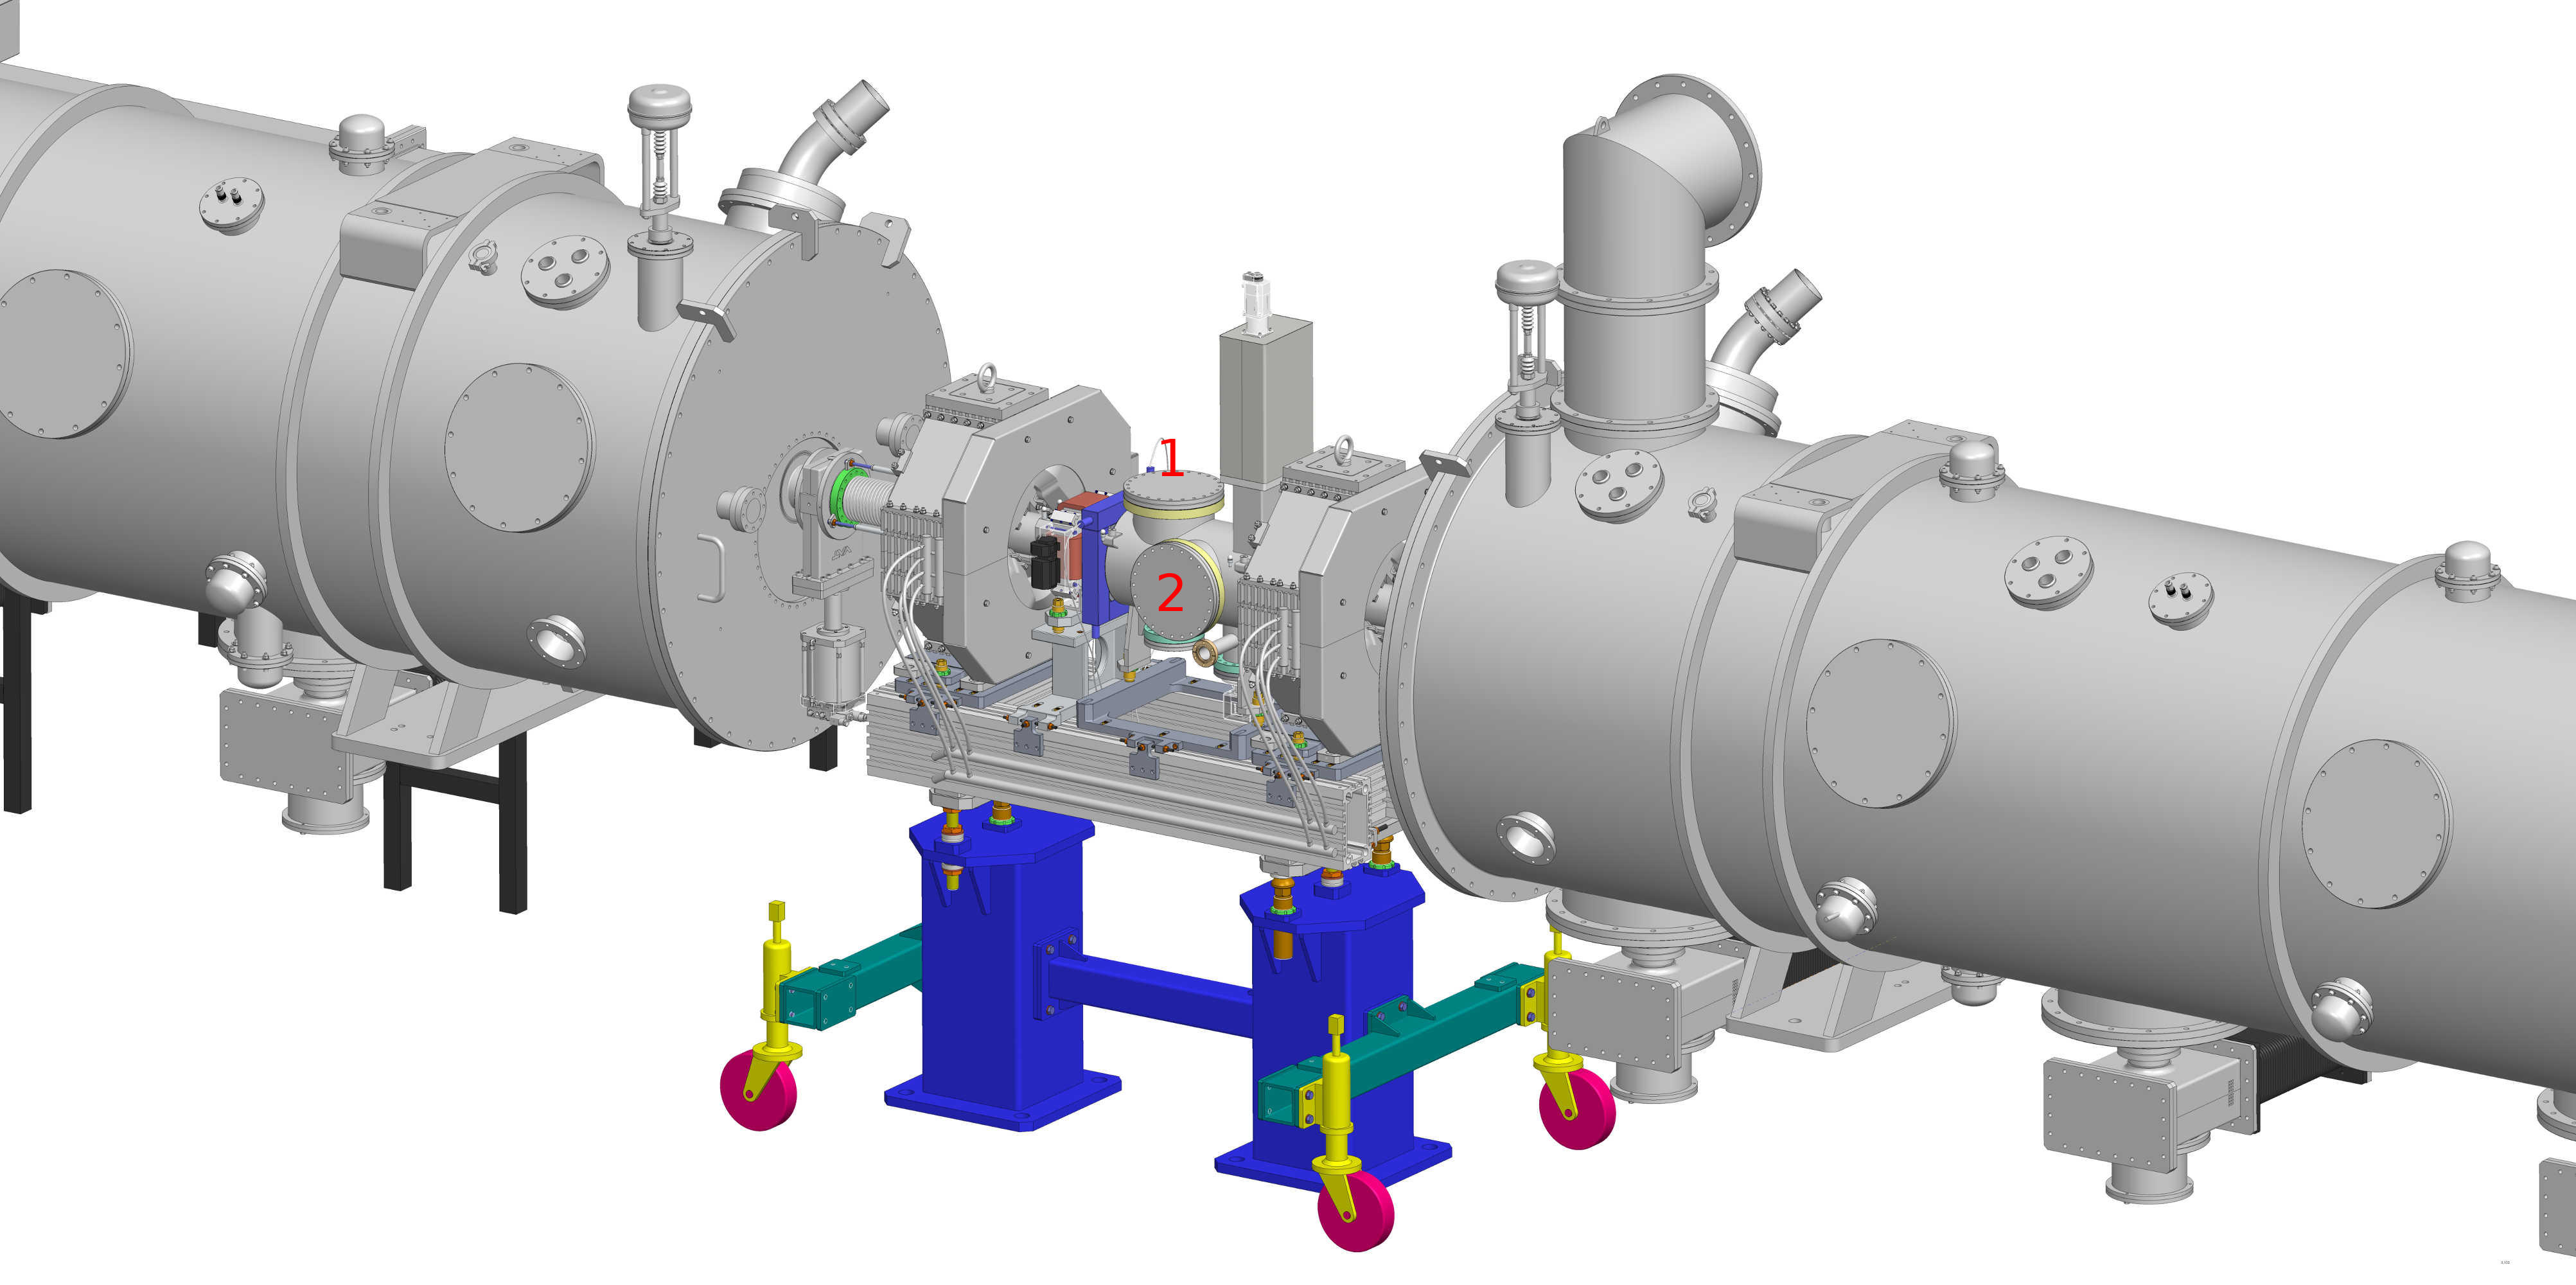
\includegraphics[width=\textwidth]{03_Prototype/figures/fig016_LWU_Cryo3.jpeg}
	\caption[The LWU vessel located between two quadrupole magnets and two cryomodules]{The LWU vessel located between two quadrupole magnets and two cryomodules. The IPMs will be mounted on the CF 200 flanges 1 and 2.}
	\label{chap3:LWU_Cryo}
\end{figure}


  The \acrshort{ipm}s will be located between two cryomodules in the cold accelerator area. The \acrshort{lwu} vessels are not cooled down, but their proximity to the superconducting cavities imposes a high vacuum level and a clean environment. Indeed, too high a pressure or a contamination may damage the cavities. An operating pressure of \(10^{-9}\,\mathrm{mbar}\) is foreseen, but the vacuum level may be even lower during the operation. Safety valves will close in case of the vacuum reaches \(10^{-7}\,\mathrm{mbar}\). Hence, quantitatively the \acrshort{ipm} design must be compliant with a high to ultra high vacuum level and an ISO-5 \cite{ISO14644} particle-free environment. Fig. \ref{chap3:LWU_Cryo} shows the \acrshort{lwu} vessel located between two cryomodules. One can see the two \acrshort{cf} 200 flanges devoted to X and Y IPMs and the two rectangular \acrshort{cf} flanges for the X and Y wire scanners.

  \section{IPM simulations overview [A]}

  \begin{wrapfigure}{r}{0.5\textwidth}
	\centering
	\begin{tikzpicture}%[scale=1.3]
		% Variables
		% Ipm
		\pgfmathsetmacro{\LIPM}{1.8};
		\pgfmathsetmacro{\HIPM}{1.8};
		\pgfmathsetmacro{\TIPM}{0.1};
		% Deg
		\pgfmathsetmacro{\LDEG}{0.1};
		\pgfmathsetmacro{\HDEG}{0.3};
		\pgfmathsetmacro{\NDEG}{6};
		\pgfmathsetmacro{\SDEG}{1.5};
		\pgfmathsetmacro{\SPAND}{(2*\SDEG - \HDEG)/\NDEG}

		\draw[] (\LIPM,0) node[right,align=left] {Field\\correctors\\or\\degraders};


		% Beam
		\draw[fill=blue!30] (0,0) circle (0.4) node[left,xshift = -0.3cm] {Beam};
		% Cage
		\draw (0,0) (-\LIPM,\HIPM)rectangle(\LIPM,\HIPM+\TIPM) node[above] {Anode};
		\draw (0,0) (-\LIPM,-\HIPM)rectangle(\LIPM,-\HIPM-\TIPM) node[below] {Cathode};
		\draw[fill=red!50] (-\LIPM/2,-\HIPM) rectangle(\LIPM/2,-\HIPM-\TIPM) node[midway,below] {Readout};
		% Ionized particle
		\draw[blue, dashed,->] (0.1,0.8)--(0.1,\LIPM);
		\draw[blue,fill=blue] (0.1,0.8) circle [radius=1mm] node[] {\tiny\color{white}{$-$}};

		\draw[red, dashed,->] (0.16,-1)--(0.16,-\LIPM);
		\draw[red,fill=red] (0.16,-1) circle [radius=1mm] node[] {\tiny\color{white}{$+$}};

		\draw[blue,dashed,->] (-0.1,0.1)--(-0.1,\LIPM);
		\draw[blue,fill=blue] (-0.1,0.1) circle [radius=1mm] node[] {\tiny\color{white}{$-$}};

		\draw[red,dashed,->] (-0.1,-0.1)--(-0.1,-\LIPM);
		\draw[red,fill=red] (-0.1,-0.1) circle [radius=1mm] node[] {\tiny\color{white}{$+$}};

		%Field
		\draw[->] (-1.2,1.5)--(-1.2,0.6) node [midway,right]{$\vec{E}$};
		% Degradors
		\foreach \x in {0,...,\NDEG}{
				\draw (0,0) (-\LIPM,\x*\SPAND - \SDEG) rectangle (-\LIPM+\LDEG,\x*\SPAND+\HDEG-\SDEG);
				\draw (0,0) (\LIPM,\x*\SPAND - \SDEG) rectangle (\LIPM-\LDEG,\x*\SPAND+ \HDEG-\SDEG);}


		%Profile
		\begin{axis}[every axis plot post/.append style={
						mark=none,domain=-3:3,samples=50,smooth},
				clip=false,
				axis y line=none,
				axis x line*=bottom,
				ymin=0,
				ymax=1,
				xtick=\empty,
				width=4cm,
				height=3cm,
				scale only axis,
				xshift=-2cm,
				yshift=-3.5cm
			]
			\addplot {\gauss{0}{0.3}{0.3}};
		\end{axis}

	\end{tikzpicture}
	\centering
	\caption[Visual explanation of how an IPM works]{Visual explanation of how an IPM works. The electric field between the electrodes can be reverted by inverting the polarity, making it possible to choose if detecting ions or electrons. Field correctors or degradors, left and right, improve the field uniformity.}
	\label{chap3:ipm_outline}
\end{wrapfigure}


  As explained in the previous chapter, an Ionization Profile Monitor (\acrshort{ipm}) is a non-invasive detector (\acrshort{npm}) that measures the transverse profile of a beam.
  Its principle of operation is shown in the Fig. \ref{chap3:ipm_outline} and can be summarized in 3 main steps:
  \begin{enumerate}
    \item Beam protons pass through the vacuum, inducing ionizations of the residual gas molecules: electron/ion pairs are created.
    \item Inside the \acrshort{ipm}, a strong electric field drives electrons or ions towards a segmented readout system.
    \item The profile is reconstructed in one transverse direction. For a complete profile, a pair of \acrshort{ipm}s, rotated by $90\textdegree{}$ with respect to each other, is mandatory.
  \end{enumerate}

  Unfortunately, there is no software that allows a full simulation of an \acrshort{ipm}. Each step requires specific tools. As a consequence, a not negligible work is necessary to link together the results obtained by the different steps of the simulations. Each simulation can be split in the 3 main parts, as reported just above. This chapter deals with all the simulations and approximations that have been developed to design our detector.

  It is important to underline that designing \acrshort{ipm}s to work in the requested conditions is really challenging. Preliminary studies were done in order to check the feasibility of the \acrshort{ipm} design. We focused our efforts on the following hot topics:
  \begin{itemize}
    \item Quantification of the ionization signal in terms of number of produced electron/ion pairs for ensuring that, in spite of the low gas pressure and tiny ionization cross section at high proton energy, the signal is sufficiently high for reconstructing a profile per pulse.
    \item The extraction field must be as uniform as possible in order to lead efficiently and correctly the ionization by-products toward the readout. %Difficulties come from the small amount of space available in the LWU.
    \item The space charge effect induced by the beam and the initial momentum of ionization electrons/ions, which may distort the profile, must be evaluated.
    \item The choice of an efficient readout technology which must match ESS working conditions.
  \end{itemize}
  All these points will be presented in the next sections.

  %  Firstly, the primary number of electron/ion pair created by the proton beam should be evaluated, and it must be sufficient in order to reconstruct a beam profile. However, this does not guaranteed that the primary particles reach the readout plane. Thus, it is necessary to perform some electromagnetic simulations. Indeed, primary particle are sensitive to the non uniformities of the extraction field and to space charge effects induced by the beam. These effects may disturb the profile measurements or reduce the number of primary particles. Therefore, they should be quantified. Lastly, the signal creation in the readout device should be evaluated with respect to previous simulations. The response of the readout mainly depends on its type.

  \section{Particle through matter [A]}
  \label{chap3:sec_particle_in_matter}
  The interactions of particles with matter are an important aspect of particle detection \cite{Knoll2010,Leo1994}. A particle will lose energy when it passes through a medium. The physical process behind the energy transfer mainly depends on the characteristics of the particle and the medium. These topics have been studied and improved over the last century. They often combine complicated theoretical laws with approximations or empirical models. This topic is very wide, hence in the following only the pertinent information for this study will be reported.

  As explained before, the \acrshort{ipm}s rely on the by-product collection of the ionized residuals gas. The number of ionized particles gives the signal strength which has to be compliant to the readout sensitivity. Therefore, we need to know how many particles are created by the beam itself along the residual gas enclosed in the accelerator beam pipe. Then we should understand how these secondary particles create a signal in the sensitive part of our \acrshort{ipm}.


  \subsection{Interaction of charged particles with matter [A]}
  For heavy charged particles, the main interaction is due to electromagnetic interactions of the incident particle with the orbiting electrons of the medium. A particle is considered heavy if its mass is much higher than the mass of an electron. The incident particle transfers a small amount of its energy to an electron of the medium at each electronic collision. In 1930, Bethe (original paper \cite{Bethe1930}) proposed an equation that describes the mean rate of energy losses per distance unit by a heavy charged particle. The so-called Bethe equation derives from coulomb interactions. This equation has been improved over years \cite{Fermi1940,Fano1963}. The expression of the linear stopping power for heavy charged particles is defined by the following equation \cite[p. 446]{Tanabashi2018}:
  \begin{equation}
    - \bigg \langle \frac{dE}{dx} \bigg \rangle =K \rho \frac{Z}{A} \frac{z^{2}}{\beta^{2}} \left[\frac{1}{2} ln \left(\frac{2 m_{e} \beta^{2} \gamma^{2} T_{max}c^{2}}{I^{2}} \right) - \beta^{2} - \frac{\delta(\beta \gamma)}{2} - \frac{C}{Z} \right]
  \end{equation}
  where \(K\) is a constant factor defined by \(K=4 \pi N_{a} r_{e}^{2} m_{e} c^{2}\), \(r_{e}\) is the classical electron radius, \(m_{e}\) is the electron mass, \(N_{a}\) the Avogadro constant and $c$ the speed of light in vacuum. For convenience, the stopping power is usually expressed in \(\mathrm{MeV/cm}\). In this case, \(K\) is equal to \(0.307075\,\mathrm{MeV \, mol^{-1} \, cm^{2}}\).

  Terms in the Bethe equation can be dissociated in two groups. First, the incident particle related terms. The maximum transfer energy for one collision is given by the following equation:
  \begin{equation}
    T_{max} = \frac{2 m_{e} \beta^{2} \gamma^{2} c^{2}}{1 + \frac{2 \gamma m_{e} }{M} + \left( \frac{m_{e}}{M} \right)^{2}}
  \end{equation}
  Where, \(M\) and \(m_{e}\) are respectively the incident particle and electron masses. The \(\beta\) and \(\gamma\) variables have their normal significance as Lorentz factors.

  Finally, the terms related to the medium. \(Z\), \(A\) and \(\rho\) are respectively the atomic number, the mass number and the density of the given medium. In most of the cases the \(\frac{Z}{A}\) ratio is close to \(0.5\) except when a medium contains hydrogen. Sometimes, the Bethe equation is given independently from the density.
  The mean excitation energy \(I\) is the only non-trivial variable in the Bethe equation \cite{Berger1984,Berger1993}. The computation is quite complicated because it requires to measure the oscillator strength for each material. Table \ref{chap3:WandI} gives the \(I\) value for common materials.

  Two correction factors are often used to improve the accuracy of the Bethe equation at low and high energies. The term \(\frac{\delta(\beta \gamma)}{2}\) corrects for the density effects at relativistic energies \cite{Sternheimer1984}. The shell correction \(\frac{C}{Z}\) improves the accuracy at low energies \cite{Bichsel2002}.

  \begin{figure}[!ht]
	\includesvg[width=\textwidth]{03_Prototype/figures/fig001_bethe_4}
	\caption[Typical mass stopping power plot a proton]{Typical mass stopping power plot for a proton. Here the mass stopping power is plotted for a proton in hydrogen and nitrogen. The calculation was done using the Bethe formula and has been cross-checked with the NIST PSTAR table which contains both computed and experimental values \cite{Seltzer1993}.}% The Bethe %equation gives correct results between \(0.2\ <\ \beta\gamma\ <\ 100\). %However at lower and higher energies the Bethe formula is no more reliable.}
	\label{chap3:bethe1}
\end{figure}


  Fig. \ref{chap3:bethe1} shows the mass stopping power of a proton in two different media. The blue region represents the energy range of protons in the cryogenic part of \acrshort{ess}, where \acrshort{ipm}s will be located. One can see that the minimum of energy loss is reached around \(2\,\mathrm{GeV}\).

  The Bethe model has been tested and improved with respect to experimental data \cite{Porter1990}. However, at very low or high energies\footnote{Below $\mathrm{MeV}$ and above hundred $\mathrm{GeV}$ for proton} the Bethe equation is no more usable. In these regions specific models are used to describe the energy loss in matter \cite{Ziegler1985, Allison1980}.

  The Bethe model is also not compatible with low mass particles like electrons and positrons. The Bethe formula must be modified for these particles \cite{Rieke1972}\cite[p. 452]{Tanabashi2018}. At low energies, electrons lose their energy by ionization like ions, whereas at energies above few \(\mathrm{MeV}\), electrons also lose energy through bremsstrahlung radiation.

  \subsection{Electron ion pairs production [A]}
  We just defined the mean energy loss rate of a charged particle per unit of distance. When a particle passes through a medium, it may transfer its energy to the medium, which for now we consider as composed of atoms not bound in molecules. If the energy is sufficient, an ionization happens: one or more electrons are ejected from the electronic shells, leading to the creation of an ion and free electron(s). In case of molecules, the ionization process may be dissociative i.e. it may break the molecular bounds. The cross section for dissociative ionization is far lower than the one for pure ionization \cite{Dimopoulou2004}.

  By introducing \(W\), the average energy for producing an ion/electron pair in a medium, we can estimate the number of ion/electron pairs created in a given readout length $\Delta x$ of materials \cite{Weiss1955,Bichsel1979} as:

  \begin{equation}
    N_{electrons}= \frac{\big \langle \frac{dE}{dx} \big \rangle}{W_{n}} \Delta x
  \end{equation}

  When an electron is ejected, it has a certain probability for ionizing other atoms when its energy is high enough. These secondary electrons are called delta rays or delta electrons. This phenomenon becomes rare and negligible when the medium has a very low density like in a vacuum system. The \(W\) parameter includes the delta ray electrons, hence the \(W\) value is biased \cite[p. 470]{Tanabashi2018} for the case at hand, since the IPMs work at very low pressure. Table \ref{chap3:WandI} gives, as an example, the \(W\) values for several materials at Normal Temperature and Pressure\footnote{$20\,\mathrm{°C}$, $1\,\mathrm{atm}$} (NTP).

  \begin{table}[ht]
	\centering
	\caption[Mean excitation energie, average energy to produce a pair and density values for severals mediums at Normal Temperature and Pressure (NTP)]
	{Mean excitation energie, average energy to produce a pair and density values for severals mediums at Normal Temperature and Pressure (NTP). Complete reviews of \(I\) and \(W\) values are available in \cite{Kamakura2006}\cite{Bichsel1979}.}
	\label{chap3:WandI}
	\begin{tabular}{llll}
		\toprule
		Gas        & \(I\) (\(\mathrm{eV}\)) & \(W\) (\(\mathrm{eV}\)) & \(\rho\) (\(\mathrm{kg/m^{3}}\)) \\
		\midrule
		\(H_{2}\)  & \(18.8\)       & \(36.43\)  &  \(0.0899\)  \\
		\(CO\)     & \(85.9\)       & \(34.5\)   &  \(1.165\)  \\
		\(CO_{2}\) & \(85.00\)      & \(34.21\)  &  \(1.842\)  \\
		\(N_{2}\)  & \(82.00\)      & \(36.39\)  &  \(1.165\)  \\
		\bottomrule
	\end{tabular}
\end{table}

  When the medium is a mixture of several compounds, its mean stopping power needs to be calculated as the sum of the mean stopping power of its components weighted by their mass proportion. As a consequence, the total number $N_{total}$ of electron/ion pairs results:
  \begin{equation}
    N_{total}= \sum_{n= First}^{Last} N_{compound\ n}= \sum_{n= First}^{Last} w_{n} \frac{\big \langle \frac{dE}{dx}\left(\rho_{n},I_{n},A_{n},Z_{n}\right) \big \rangle}{W_{n}} \Delta x
  \end{equation}
  The calculation can be done for each single element or for each molecule in the compound.
  This latter is recommended since the \(I\) values are in general higher for molecules \cite[p. 451]{Tanabashi2018}.

  \subsection{Calculation [B]}
  \label{chap3:calc}
  Following the physics introduction reported above, this subsection is dedicated to the estimation of the number of primary particles that will be created at the \acrshort{ess} conditions. We tried two different approaches: naive computation of Bethe equation and simulations through a software.

  The Bethe formula can be implemented in a spreadsheet or a C++ code once the composition of the medium and the \(I\) value of each compound is known. The expected pressure in the cryogenic part at \acrshort{ess} is around \(10^{-9}\,\mathrm{mbar}\), and the gas composition is given in Table \ref{chap3:ess_vacuum_gas}.

  \begin{table}[ht]
	\centering
	\caption[Expected residual vacuum gas in the cold part of ESS Linac, provided by ESS vacuum group]
	{Expected residual vacuum gas in the cold part of ESS Linac, provided by ESS vacuum group.}
	\label{chap3:ess_vacuum_gas}
	\begin{tabular}{llll}
		\toprule
		Gas        & Mass percentage (\(\%)\) & $p_{i}$ (\(\mathrm{mbar}\)) & $\rho_{i}$ $(\mathrm{g/cm^{3}}$) \\
		\midrule
		\(H_{2}\)  & \(79\)          & \(7.9 10^{-10}\)   & \(6.52\cdot
		10^{-17}\)                                                                \\
		\(CO\)     & \(10\)          & \(1.0 10^{-10}\)   & \(1.15\cdot
		10^{-16}\)                                                                \\
		\(CO_{2}\) & \(10\)          & \(1.0 10^{-10}\)   & \(1.8\cdot
		10^{-16}\)                                                                \\
		\(N_{2}\)  & \(1\)           & \(1 10^{-11}\)     & \(1.14\cdot
		10^{-17}\)                                                                \\
		\bottomrule
	\end{tabular}
\end{table}

  We assume that the residual gas follows the "perfect gas" law. We also assume that the linear density scaling of Bethe equation remains true in high vacuum \cite[p. 108]{egber2012}\cite{Ishimaru1995}. Hence, the partial pressure and the density for each gas is calculated with respect to the tabulated pressures. The primary signal is computed at \acrshort{ess} nominal conditions given in Table \ref{chap2:ess_charac}.

  Fig. \ref{chap3:ess_primary_particles} shows the number of electron ion pairs created for each gas species versus the \acrshort{ess} proton beam energy. The different \acrshort{ipm}s locations are marked by a blue line. One can see that the gas density has a strong influence on the primary signal. Although the hydrogen is the main species in terms of proportion, its contribution to the signal is close to the one from carbonate species. Note that the \(W\) value may overestimate the number of pairs created due to secondary delta rays.

  \begin{figure}[!ht]
	\includesvg[width=\textwidth]{03_Prototype/figures/fig015_ess_primary_particle}
	\caption[Expected number of electron/ion pairs per centimeter at ESS nominal conditions according to Bethe equation]{Expected number of electron/ion pairs per centimeter at ESS nominal conditions according to Bethe equation. Each vertical line corresponds to an IPM location.}
	\label{chap3:ess_primary_particles}
\end{figure}


  We have also used the Garfield++ software to compute the number of primary  ionizations. This software is normally intended for the modelization of gaseous detectors. It allows to simulate the creation of electron/ion pairs due to the ionization of gas by an incident particle, the transport and amplification of these electrons in the gas and the signal induced on a readout plane. In our case, we simulated only the pair creation in the residual gas. For this step Garfield++ uses two programs internally:
  \begin{itemize}
    \item Magboltz: a Fortran routine that compute different properties of a gas mixture and performs the transport of electrons in this mixture \cite{Biagi1989}.
    \item Heed ++ \cite{Smirnov2005}: a C ++ code that implements an ionization model based on the photoabsorption ionization (PAI) \cite{Allison1980}.
  \end{itemize}

  \begin{table}[ht]%{r}{0.5\textwidth}
	\centering
	\caption[Comparison of expected number of electrons between calculation using Bethe equation and results from Garfield++.]
	{Comparison of expected number of electrons between calculation using Bethe equation and results from Garfield++}
	\label{chap3:GarfieldBethe}
	\begin{tabular}{llll}
		\toprule
		Energy    & \(N_{Bethe}\) & \(N_{garfield}\) & Factor \\
		\midrule
		\(97.2\)  & \(100210\)    & \(52537\)             & \(0.52\)   \\
		\(231.4\) & \(54970\)     & \(27463\)             & \(0.50\)   \\
		\(278.9\) & \(49160\)     & \(26124\)             & \(0.53\)   \\
		\(315.8\) & \(45850\)     & \(23769\)             & \(0.52\)   \\
		\(628.3\) & \(33600\)     & \(17522\)             & \(0.52\)   \\
		\bottomrule
	\end{tabular}
\end{table}
  A dummy detector, a cube of ten centimeter side, is implemented and filled with the same gas composition as the ESS residual gas. Protons are shot into this detector and the information on the electrons created in the gas is saved in a ROOT file \cite{Brun1997,Antcheva2009} for post processing. This is done for different proton energies and vacuum levels.

  The Table \ref{chap3:GarfieldBethe} reports the value of expected number of electrons/ions pairs per cm obtain from the direct calculation (Bethe equation) and from the results of the Garfield++ simulations. One can see that the Garfield++ value is always lower than the calculation by a constant factor $0.52$.


  \subsection{Pressure uniformity [A]}

  The primary signal is strongly dependent on the pressure inside the vacuum chamber. A gradient in the pressure may cause a change in the signal shape. It is therefore interesting to simulate the vacuum level in the LWU to check the existence of such gradient in the residual gas of the IPMs.

  \begin{wrapfigure}{r}{0.5\textwidth}
  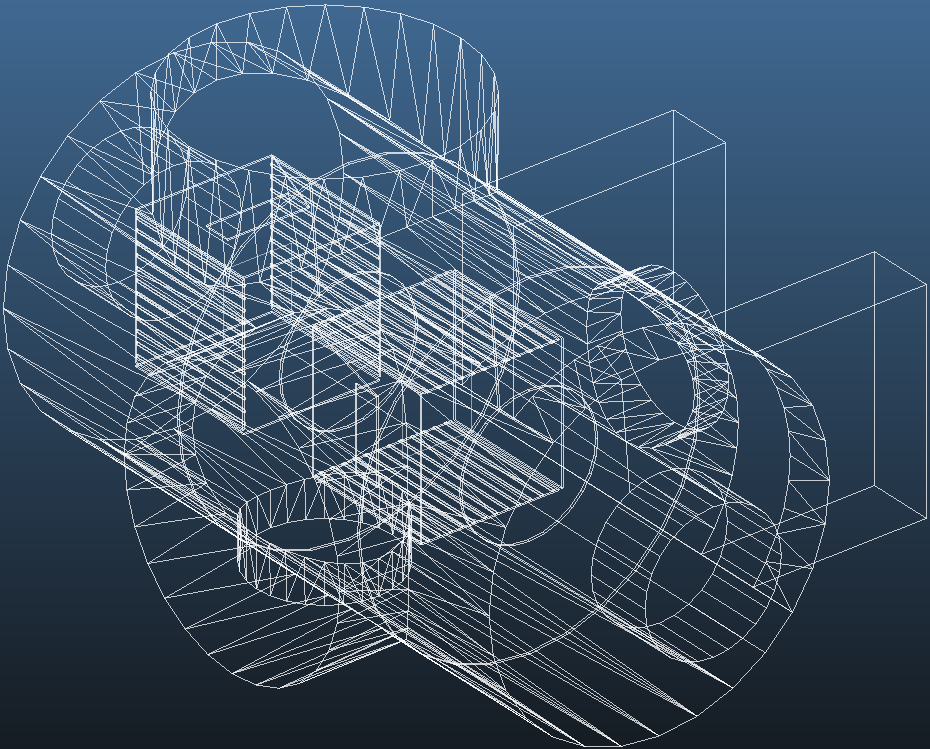
\includegraphics[width=0.5\textwidth]{03_Prototype/figures/fig019_molflow_LWU.png}
  \caption[The LWU geometry implemented in Molflow+]{The LWU geometry implemented in Molflow+.}    
	\label{chap3:molflow_LWU}
\end{wrapfigure}


  A simulation has been done with the Molflow+ software developed at CERN \cite{Kersevan2009}. It simulates the vacuum in a steady state by using Monte Carlo and Ray Tracing methods. The user defines his geometry, as well as the desorption and adsorption rates of each surface. As visible in Fig. \ref{chap3:molflow_LWU}, the implemented geometry does not contain all the structures and surfaces. Two dummy squares facets of $5\,\mathrm{cm}$ side are inserted in the center of each \acrshort{ipm}. The pressure profiles are then measured on these facets. No information about the real pumping speed, surface conditions or other vacuum characteristics is input in the program, therefore the simulation is not done for determining the vacuum achievable by our system in the LWU but to verify the uniformity of the pressure profile in both \acrshort{ipm}s. We also checked the case of a unwanted outgassing occuring on one side of the IPMs. No significant change has been observed.

  \begin{figure}[!h]
	\begin{center}
		\includesvg[width=\textwidth]{03_Prototype/figures/fig020_profile_pressure}
	\end{center}
	\caption[Simulated profile pressure in the center of IPMs.]{Simulated profile pressure in the center of IPMs.}
	\label{chap3:profile_pressure}
\end{figure}


  Fig. \ref{chap3:profile_pressure} shows the results from the simulations. The pressure levels seem to be uniform for the 2 IPMs along the transverse direction, and it may not affect the profile measurement. The pressure is slightly lower in the second IPM because the pumping group is closer.

  \section{Extraction field [B]}
  \begin{wrapfigure}{r}{0.5\textwidth}
	\centering
	\begin{tikzpicture}
		% Variables
		% Ipm
		\pgfmathsetmacro{\LIPM}{1.8};
		\pgfmathsetmacro{\HIPM}{1.8};
		\pgfmathsetmacro{\TIPM}{0.1};
		% Deg
		\pgfmathsetmacro{\LDEG}{0.1};
		\pgfmathsetmacro{\HDEG}{0.3};
		\pgfmathsetmacro{\NDEG}{6};
		\pgfmathsetmacro{\SDEG}{1.5};
		\pgfmathsetmacro{\SPAND}{(2*\SDEG - \HDEG)/\NDEG}

		% Beam
		\draw[fill=blue!30] (0,0) circle (0.4) node[left,xshift = -0.3cm] {Beam};
		% Cage
		\draw (0,0) (-\LIPM,\HIPM)rectangle(\LIPM,\HIPM+\TIPM) node[above] {Anode};
		\draw (0,0) (-\LIPM,-\HIPM)rectangle(\LIPM,-\HIPM-\TIPM) node[below] {Cathode};
		\draw[fill=red!50] (-\LIPM/2,-\HIPM) rectangle(\LIPM/2,-\HIPM-\TIPM) node[midway,below] {Readout};
		% Ionized particle
		\draw[blue, dashed,->] (0.1,0.8)to [bend right=15](-0.1,\LIPM);
		\draw[blue,fill=blue] (0.1,0.8) circle [radius=1mm] node[] {\tiny\color{white}{$-$}};

		\draw[red, dashed,->] (0.36,-1)to [bend left=0](0.56,-\LIPM);
		\draw[red,fill=red] (0.36,-1) circle [radius=1mm] node[] {\tiny\color{white}{$+$}};

		\draw[blue,dashed,->] (-0.1,0.1)to [bend right=15](-0.8,\LIPM);
		\draw[blue,fill=blue] (-0.1,0.1) circle [radius=1mm] node[] {\tiny\color{white}{$-$}};

		\draw[red,dashed,->] (-0.1,-0.1)to [bend right=15](0.2,-\LIPM);
		\draw[red,fill=red] (-0.1,-0.1) circle [radius=1mm] node[] {\tiny\color{white}{$+$}};

		%Field
		\draw[->] (-1.2,1.5)--(-1,0.6) node [midway,right]{$\vec{E}$};

		% Profile
		\begin{axis}[every axis plot post/.append style={
						mark=none,domain=-3:3,samples=50,smooth},
				clip=false,
				axis y line=none,
				axis x line*=bottom,
				ymin=0,
				ymax=1,
				xtick=\empty,
				width=4cm,
				height=3cm,
				scale only axis,
				xshift=-2cm,
				yshift=-3.5cm
			]
			\addplot {\gauss{0.75}{0.5}{0.3}};
		\end{axis}
	\end{tikzpicture}
	\centering
	\caption[Non-uniformities leading to mirage effects on the profile measurement]{Non-uniformities leading to mirage effects on the profile measurement.}
	\label{chap3:FieldNonU_outline}
\end{wrapfigure}

  The \acrshort{ipm}s can be seen as parallel plate detectors. In an ideal \acrshort{ipm} these plates are infinite sized. The extraction field is then completely oriented in a single direction, normal to the detection plane and the projection of the profile on this plane is perfect. In reality, the plates have finite dimensions, comparable to the gap between the two electrodes. In these conditions the field is no more uniform.

  The effects induced by the cage sides are no longer negligible; field uniformity is strongly influenced by the needle effects of the plates.
  Also, the geometry of the vacuum chamber affects on the field uniformity: it is considered to be at ground but walls close to the \acrshort{ipm}s modify change the electric field lines inside the \acrshort{ipm}s. In addition, the cross-interaction between the electric fields of two close by IPMs is very strong.

  Finally, the way to create the field with high voltage (\acrshort{hv}) power supplies has an important influence on the field itself. We will see later that some readouts can only work in certain configurations of high voltage, unless major modifications of the set-up are considered.

  The non-uniformity of the electric field is very problematic because it creates mirage effects and prevents the correct measurement of the beam profile as shown in Fig. \ref{chap3:FieldNonU_outline}. It also determines the maximum size of the detection area, which must be in a zone where the electric field is as uniform as possible. To overcome the mirage effect, the field line must be as straight as possible. Several solutions can be considered to improve the field uniformity:
  \begin{itemize}
    \item The distance between the two electrodes can be reduced. In this case, the \acrshort{ipm}s will tend to a configuration close to the infinite parallel plates assumption. Following the same logic, the size of both electrodes could be increased. Theses solution are mainly limited due to mechanical considerations. To stay on the safe side, the distance between two plates was chosen to be at least equal to the diameter of the beam pipe. Moreover, the whole assembly of one \acrshort{ipm} must hold on a CF 200 flange.
    \item Using field correctors or field degraders \cite[p. 103]{egber2012}. This is done by placing conductors on each side. Each corrector is set to a certain potential in order to constrain the field. This solution is easy to implement, compact, and very versatile. However, it requires a large number of \acrshort{hv} feedthroughs or the use of resistors in vacuum. The longitudinal field can also slightly improved in a same way.
    \item Putting grounded conductors between the two \acrshort{ipm}s \cite[p. 132]{egber2012} to protect against the \acrshort{ipm} cross-interaction. The longitudinal correctors also reduced the cross-interaction.
    \item Optimizing the geometry of \acrshort{hv} electrodes. For example, with a curved geometry with reinforcements on the edges it is possible to correct the field transversely and longitudinally \cite{Bartkoski2014}. Hence, there is no more need of field correctors.
  \end{itemize}
  Aside the above listed solutions, software corrections may be a way to correct the non uniformities. However, as previously explained the non-uniformity of the extraction field is not the only phenomenon responsible for the distortions of the measured profile. It is therefore extremely difficult to implement it, because it requires a perfect mapping of the extraction field to decouple it from other phenomena. Physical corrections are simpler to implement.

  % The second limitation concerns possible \acrshort{hv} breakdowns. In very high vacuum a distance of some millimeter is sufficient to isolate several tens of kilovolts. However, the breakdowns are also strongly influenced by the surface states of the electrodes, the composition of the vacuum and the presence of leakage current \cite{Latham1995}. Hence, we should keep a standoff distance between the electrode and the vacuum vessel (less than 1kV/cm between the IPMs and LWU).

  \subsection{Maxwell equations at steady state [A]}
  Electric and magnetic fields are perfectly described by the Maxwell's equations. Since we are in vacuum, the Maxwell's equations can be reduced to:
  \begin{alignat*}{3}
    \overrightarrow{\nabla} \cdot \overrightarrow{E}  & = \frac{\rho}{\epsilon_{0}}\quad                                           &  & \text{(Maxwell-Gauss's Law)}   \\
    \overrightarrow{\nabla} \times \overrightarrow{E} & = - \frac{\partial \overrightarrow{B}}{\partial t}\quad                    &  & \text{(Maxwell-Faraday's Law)} \\
    \overrightarrow{\nabla} \cdot \overrightarrow{B}  & = 0\quad                                                                   &  & \text{(Maxwell-Thomson's Law)} \\
    \overrightarrow{\nabla} \times \overrightarrow{B} & = \overrightarrow{J} + \frac{\partial \overrightarrow{E}}{\partial t}\quad &  & \text{(Maxwell-Ampère's Law)}
  \end{alignat*}

  The time derivatives cancel, when the field variations over time are negligible compared to the studied phenomena. So, the coupling effects between the electric and the magnetic fields disappear. Therefore, the electrostatic field depends only on the Gauss’s law. In electrostatic, it is quite convenient to introduce the electric potential:
  \begin{equation}
    \vec{E} = - \vec{\nabla}V
  \end{equation}

  \subsection{Solving Poisson's equation [B]}
  The electric potential follows the Poisson's equation:
  \begin{equation}
    \vec{\nabla}^{2}V = -\frac{\rho}{\epsilon_{0}}
  \end{equation}
  or in a more generic notation:
  \begin{equation}
    \Delta v = f
  \end{equation}
  with $f$ the right hand side function.

  The solution of this equation can be found analytically, by relying on the use of complex numbers or Laplace transforms. However, when the size of the problem increases the solution becomes harder to compute, and solving the Poisson's equation on complicated domains is almost impossible. Numerical methods allow to approximate the solutions of partial differential equations (\acrshort{pde}) on non trivial domains. There are many schemes to solve numerically \acrshort{pde}. In this section we will briefly present three methods that are often used. It is important to understand how they work and to know their limitations or pitfalls. In numerical schemes, the domain is discretized in a finite set of points. Then, the solution is approximated at each point with respect to initial and/or boundary conditions. To solve a problem, it must be well posed: the problem must admit a single unique solution that depends continuously on the variables and conditions \cite{Hadamard1902}. It turns out that the Poisson's equation is a well-posed problem if a Dirichlet condition is applied.

  %\paragraph{}
  Finite Difference Method (FDM) is a popular way to solve numerically the Poisson’s equation. In FDM, the domain is discretized regularly with a step $h$. The Taylor's theorem allows to approximate the value of a function by a polynomial equation that depends on its derivatives nearby:
  \begin{align}
     & v(x+h) = v(x)+hv^{\prime}(x)
    +\frac{h^2}{2}v^{\prime\prime}(x)+\frac{h^3}{6}v^{\prime\prime\prime}(x) + O(h^{4}) \\
     & v(x-h) = v(x)-hv^{\prime}(x)
    +\frac{h^2}{2}v^{\prime\prime}(x)-\frac{h^3}{6}v^{\prime\prime\prime}(x) + O(h^{4})
  \end{align}
  From these formulas, the second derivative can be expressed:
  \begin{equation}
    \frac{\partial^{2} v}{\partial x^{2}} = \frac{v(x+h) - 2 v(x) + v(x-h)}{h^{2}} + O(h^{2})
  \end{equation}
  and in case of a two-dimensional domain it is written as follows:
  % h^{2}v^{\prime\prime}(x,y)=
  \begin{equation}
    \begin{split}
      \Delta v & = \frac{\partial^{2} v}{\partial x^{2}} + \frac{\partial^{2} v}{\partial y^{2}} \\
      &= \frac{v(x+h,y) + v(x-h,y)
        + v(x,y+h) + v(x,y-h)
        - 4v(x,y)}{h^2} + O(h^{2})
    \end{split}
  \end{equation}
  Each point of the domain can be expressed according to its neighbors. Then, it is possible to write a set of linear equations in matrix form by choosing wisely the indexing order. For example, when the domain is decomposed line by line, one can obtain the same system of equations repeated for each inner line \footnote{The first and last lines have a slightly different set of equations due to boundary conditions.}.
  \begin{equation}
    Id \cdot v_{u} + A \cdot v_{c} + Id \cdot v_{d} = D
  \end{equation}
  Where $Id$ is the identity matrix, $v_{u}$ are the unknown values of the upper line, $v_{d}$ of the lower line, $v_{c}$ of the current line, $ A =
    \begin{pmatrix}
      -4     & 1      & 0      & \cdots \\
      1      & -4     & 1      & \cdots \\
      0      & 1      & -4     & \cdots \\
      \vdots & \vdots & \vdots & \ddots
    \end{pmatrix} $ is the square matrix of FDM schemes and $D$ is vector of Dirichlet values. Then, the global matrix is assembled by combining the sub-matrices for each line.
  \begin{equation}
    \begin{bmatrix}
      A      & Id     & 0      & \cdots \\
      Id     & A      & Id     & \cdots \\
      0      & Id     & A      & \cdots \\
      \vdots & \vdots & \vdots & \ddots
    \end{bmatrix}
    \cdot
    \begin{bmatrix}
      v \\
      v \\
      v \\
      \cdots
    \end{bmatrix}
    =
    \begin{bmatrix}
      D \\
      D \\
      D \\
      \cdots
    \end{bmatrix}
  \end{equation}
  On can see that the problem is solved by inverting the A matrix. This matrix is very sparse and can be inverted with iterative methods rather than a direct inversion. FDM is straightforward and allows to quickly solve Poisson’s equation on a linear structured mesh. For instance, it is very useful for calculating an electric field generated by a charge density. However, FDM cannot be used when the geometry becomes too complex.

  \paragraph{}
  The Finite Element Method (FEM) is more suitable for solving PDE on complex domains. The FEM uses the weak formulation of the Poisson’s equation. By introducing a test function $\varphi$, this weak form can be written easily thanks to an integration by parts:
  \begin{align}
    \int_{\Omega}^{} \varphi \Delta v d\Omega                                                                                           & = \int_{\Omega}^{} \varphi f d\Omega \\
    -\int_{\Omega}^{} \vec{\nabla} \varphi \cdot \vec{\nabla} v d\Omega + \int_{\Sigma}^{} \varphi \vec{\nabla} v \cdot \vec{n} d\Sigma & = \int_{\Omega}^{} \varphi f d\Omega
  \end{align}
  with $\Sigma$ boundary domain.
  One can see that the Laplacian disappeared from the formulation. An approximation of $v$ is done in the reduced domain by mean of low order polynomial functions. Again, a finite system of linear equations can be written, and the problem is solved by inverting the matrix. The correct choice of test functions and the way to index elements lead to very sparse matrix which can be inverted easily. Unlike the FDM, the solution is approximated on the whole reduced domain and not locally. FEM supports complicated meshes as long as they are continuous and solves all kinds of PDEs that may be much more complex than the Poisson’s equation.

  \paragraph{}
  % Expliquer mieux les BEM
  With FEM, the whole domain is fully discretized and. In case of electrostatic field, it is possible to use the Boundary Element Method (BEM). With the BEM, the Poisson’s equation is first solved on boundaries. Then, the electric field can be evaluated at any point in the domain from the contributions of all boundaries. The discretization is also performed only on the boundaries and not on the entire geometry. So, the dimension of the problem is reduced and the matrix to be reversed is much smaller. On the other hand, the matrix is ​​no longer sparse.

  Most of the commercial simulation softwares \cite{cststudio2018,ansys2018,couloumb2018} rely on FEM or BEM. We have used mainly COMSOL software for the simulations of extraction fields.

  \subsection{COMSOL [A]}
  COMSOL is a commercial all-in-one multi-physics simulation software able to solve various problems from structural mechanical analysis to optical raytracing \cite{comsol2018}. We use COMSOL with the AC/DC module \cite{comsolacdc2018} to simulate the static electric field in the \acrshort{ipm} box. COMSOL allows to quickly define, simulate and post process physical model. The typical workflow is divided in three main steps as follow.

  \paragraph{}
  The first step is to implement the detector geometry into COMSOL. The software includes basic \acrshort{cad} features allowing to quickly create two or tridimensional geometries. The users can directly import a mesh from files generated by external \acrshort{cad} tools. Care should be taken from importing a \acrshort{cad} file: it often contains many details and thus increases the CPU time consumption. It is much faster to directly implement the geometry with COMSOL.  In our case, only the inner shape of the vacuum chamber and the \acrshort{ipm}s must be defined. All other conductive bodies that enclose the vacuum are not relevant for an electrostatic simulation. Therefore, the geometry can be simplified. Fig. \ref{chap3:COMSOL_LWU} shows, on the left, a 3D drawing of the \acrshort{ess} vacuum vessel with the two \acrshort{ipm}s inside. And on the right, an example of the simplified geometry implemented in COMSOL.

  \begin{figure}[ht]
	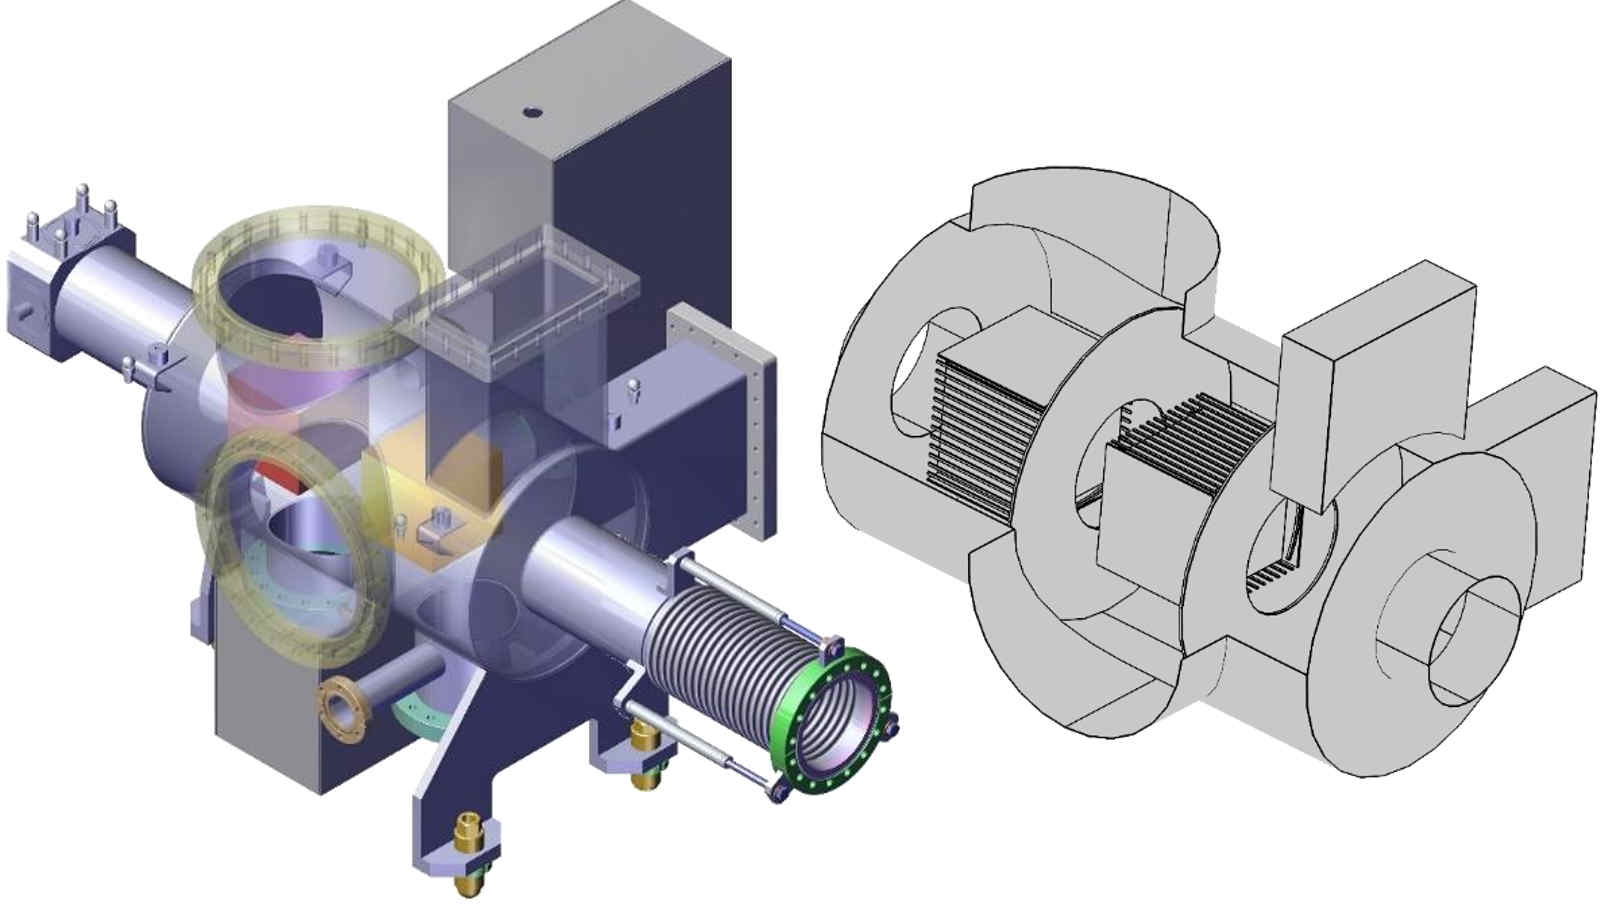
\includegraphics[width=\textwidth]{03_Prototype/figures/fig003_COMSOL_LWU.jpeg}
	\caption[A drawing of LWU (left) and its implementation in COMSOL (right)]{A drawing of LWU (left) and its implementation in COMSOL (right).}
	\label{chap3:COMSOL_LWU}
\end{figure}


  \paragraph{}
  The next step consists in the discretization of the previous geometry in many Lagrange elements in order to form a mesh. Fig. \ref{chap3:COMSOL_meshing_elements} shows the main meshing elements available in COMSOL. For an electrostatic tri-dimensional study, COMSOL uses quadratic tetrahedral elements by default. The meshing algorithm tries to create elements fitting well the geometry. For the inner small parts of the geometry, the size of elements will be reduced. Conversely, mesh cells will become bigger and bigger in coarse regions of the geometry. This behavior is not desirable for us, since the \acrshort{ipm} region of interest has no geometrical variations. The geometry would not be not described accurately. Fortunately, the user can change the characteristics and the nature of the elements in specific regions of the defined geometry. We used a tetrahedral mesh everywhere but in the \acrshort{ipm} box, where a cubic mesh with high granularity is defined. The meshing step is very memory consuming, but a poorly optimized mesh may destroy performances.

  \begin{figure}[ht]
	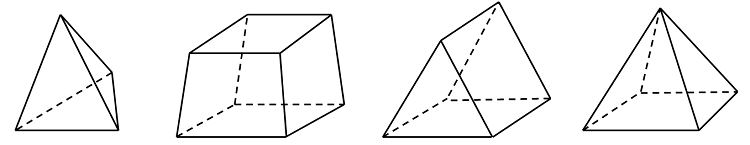
\includegraphics[width=\textwidth]{03_Prototype/figures/fig006_COMSOL_meshing_elements.png}
	\caption[3D Mesh elements included in COMSOL]{Mesh elements included in COMSOL software. From left to right: tetrahedron, hexahedron, prism and pyramid \cite{mesh2013}. COMSOL uses tetrahedral elements by default to mesh a 3D geometry in AC/DC module.}
	\label{chap3:COMSOL_meshing_elements}
\end{figure}


  \paragraph{}
  The last step is to define boundary conditions. COMSOL hides completely the mathematical aspect of the \acrshort{fem}/\acrshort{bem} and directly expresses the boundary conditions by associating them a physical meaning. This means that, when using AC/DC module, the user should fix potentials or charge densities on boundaries. A more detailed description of each boundary condition type can be found in the reference manual. COMSOL is able to solve electrostatic problems by means of \acrshort{fem} or \acrshort{bem} since version 5.3a. We compared the \acrshort{fem} and \acrshort{bem} for same configurations and we found out that results are slightly different as shown in Fig. \ref{chap3:FEMvsBEM}. We decided to use mainly \acrshort{fem} since it is the legacy method in COMSOL.
  Once solved, the results can be visualised directly in COMSOL. Data can be also exported to an external file in text format (comma separated values or VTU format).

  \begin{figure}[!h]
	\begin{subfigure}{.5\textwidth}
		\centering
		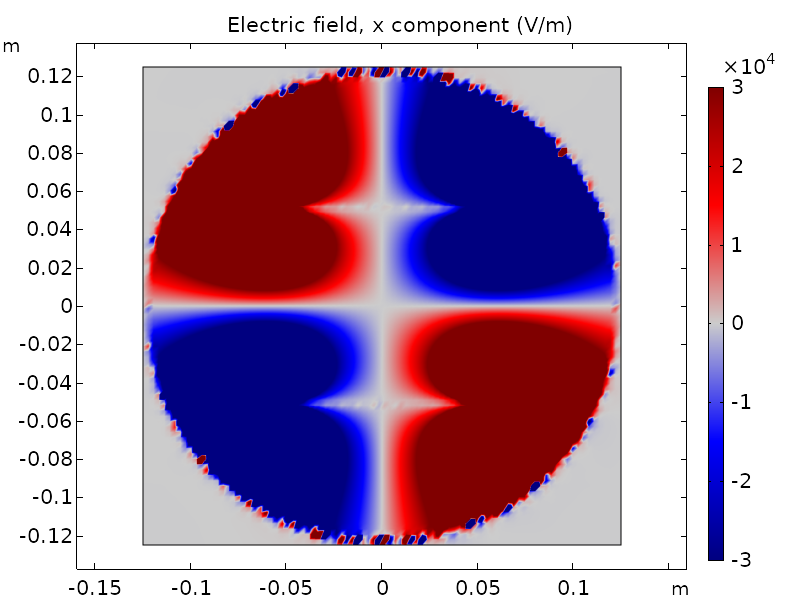
\includegraphics[width=\textwidth]{03_Prototype/figures/fig012_BEMa.png}
		\caption{Configuration 1 solved with BEM.}
		\label{}
	\end{subfigure}\hfill
	\begin{subfigure}{.5\textwidth}
		\centering
		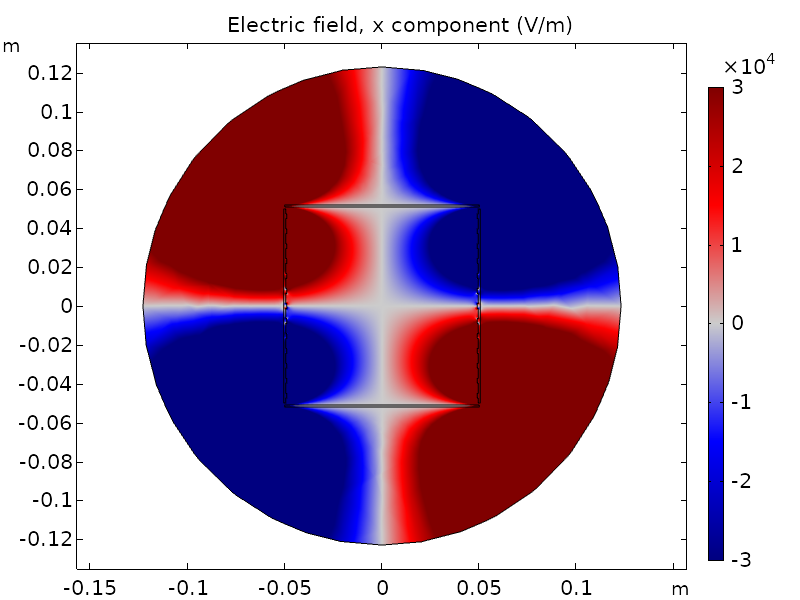
\includegraphics[width=\textwidth]{03_Prototype/figures/fig012_FEMa.png}
		\caption{Configuration 1 solved with FEM.}
		\label{}
	\end{subfigure}
	\vskip\baselineskip
	\begin{subfigure}{.5\textwidth}
		\centering
		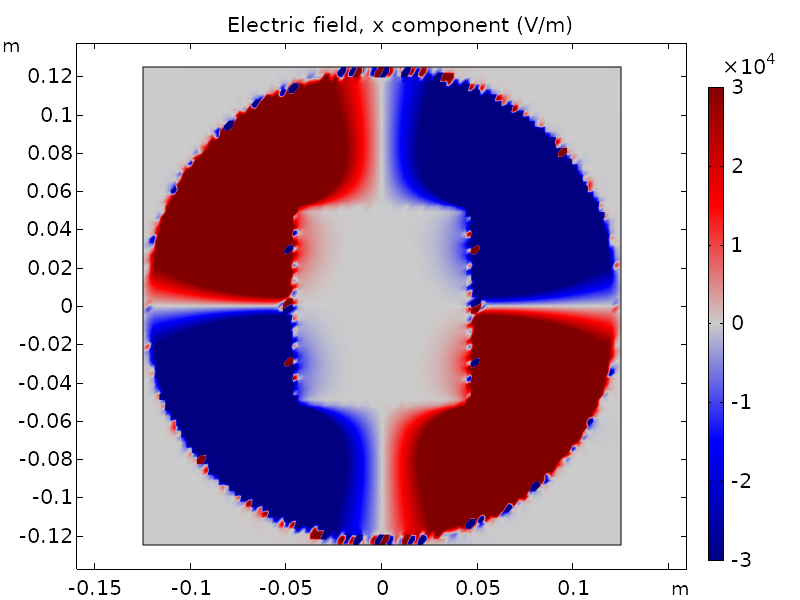
\includegraphics[width=\textwidth]{03_Prototype/figures/fig012_BEMb.png}
		\caption{Configuration 2 solved with BEM.}
		\label{}
	\end{subfigure}\hfill
	\begin{subfigure}{.5\textwidth}
		\centering
		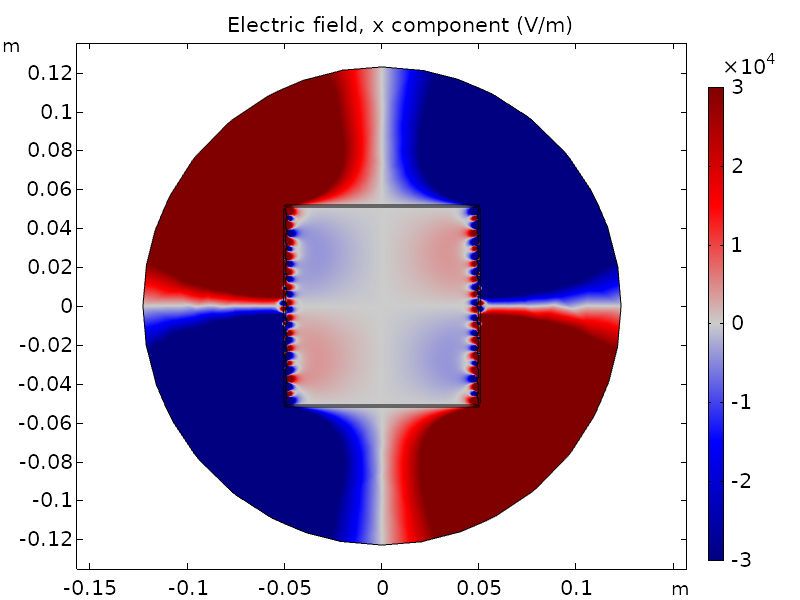
\includegraphics[width=\textwidth]{03_Prototype/figures/fig012_FEMb.png}
		\caption{Configuration 2 solved with FEM.}
		\label{}
	\end{subfigure}
	\caption[Comparison beetwen BEM and FEM for two different IPM configurations]{Comparison beetwen BEM and FEM for two different IPM configurations.}
	\label{chap3:FEMvsBEM}
\end{figure}


  \paragraph{}
  Here below the relevant assumptions made in our COMSOL model are listed:
  \begin{itemize}
    \item All conductors and insulators are supposed to be perfect.
    \item Field correctors and electrodes are thicker than in reality since it is not feasible to describe a micrometer deposition layer in a meter scale simulation.
    \item Neither the resistor chain at the back of field correctors, not the connection wires, feedthroughs and connectors are implemented.
    \item The vacuum vessel is supposed to be at the same ground as the power supplies, and without any charge on its surface.
  \end{itemize}

  \subsection{Criteria [B]}

  It is necessary to define criteria to quantify the uniformity of the electric field in order to compare several simulations together. In this thesis, we will use mainly:
  \begin{itemize}
    \item Visual approaches (isocolors and streamlines) that are sufficient at first to underline big differences between two models.
    \item A statistical criterion
    \item Particle tracking
  \end{itemize}
  In this section, we will explain briefly the two last criteria.

  \paragraph{}
  For the statistical criterion, the whole data set is sliced in the longitudinal direction. In each slice, the quadratic mean value of each electric field component is computed in an small cylinder at the center of the IPM.
  \begin{equation}
    \vec{E}_{mean} = \frac{\sum_{i=1}^{N}\sqrt{\vec{E}_{i}^{2}}}{N}
  \end{equation}
  The only pitfall of this method is the size of the area. The mean value must be computed on an area that covers at least the beam\footnote{We assume that the beam is centered}. On the other hand, if the area is too big, then the mean value will be biased due to field correctors on each side of the IPMs.
  To choose the area size, we proceed as follows. A charged particle is released at rest in a dummy IPM where the field is perfectly uniform except in a small region. In this region, we add a component perpendicular to the field lines and equal to $1\,\mathrm{\%}$ of the main field value. When the particle reaches the readout, the total deviation is recorded. Then the region is shifted and the computation is repeated. Table \ref{chap3:Deviation} tabulates results.

  \begin{table}[ht]
	\centering
	\caption[Example of deviation of the trajectory of a particle in an IPM]
	{Example of deviation of the trajectory of a particle in an IPM. A particle is released in the center of an IPM with a straight field everywhere, but in a certain range a parasitic field component is added and set to $1\,\mathrm{\%}$ of the main field. The 0 coordinate is the IPM center whereas the readout is at \(5 \, \mathrm{cm}\) distance.}
	\label{chap3:Deviation}
	\begin{tabular}{cccccc}
		\toprule
		                               & \multicolumn{5}{c}{Range (\(\mathrm{cm}\))}                                                 \\
		\cmidrule(lr){2-6}
		                               & \([0,1]\)                                   & \([1,2]\) & \([2,3]\) & \([3,4]\) & \([4,5]\) \\
		\midrule
		Deviation (\(\mathrm{\mu m}\)) & \(347\)                                     & \(85\)    & \(42\)    & \(20\)    & \(5.6\)   \\
		\bottomrule
	\end{tabular}
\end{table}

  One can see that the deviation is quite important when the particle has almost no kinetic energy, i.e. when the particle is created.
  At the end of the drift, the particle has far higher kinetic energy and is therefore less affected by field non-uniformities. This means that, the field must be optimized to be as much uniform as possible at the center of the IPM. The non-uniformities on the IPM sides are less of a concern.
  So we decided to compute the quadratic mean inside a circle of at least $2\,\mathrm{cm}$ radius. However, it is impossible to predict the real effects on the profile since the quadratic mean shadows the direction of the field.

  \paragraph{}
  The tracking algorithm is, in theory, the most relevant criterion for an IPM. Charged particles are released in the center of the IPM and we observe them drifting in the field cage along the field lines generated by the electric and magnetic fields, thanks to Lorentz’s force:
  \begin{equation}
    \vec{F} = m \cdot a = q \cdot (\vec{E}(\vec{r},t) + \vec{v} \times \vec{B}(\vec{r},t))
  \end{equation}
  Once the tracking is done the relative error on $\sigma$ can be computed:
  \begin{equation}
    \left| \Delta \sigma_{beam} \right| = \left|\frac{\sigma_{final} - \sigma_{initial}}{\sigma_{initial}} \right|
  \end{equation}
  Initial particle positions are drawn following an ESS pulse shape with well defined longitudinal and time characteristics. The equation of motion is integrated with a numerical integrator. The value of the field at an arbitrary position is interpolated from values computed by COMSOL. These steps are repeated until the particles reach the detection system. The simplest numerical method is probably the Euler integration, written as follow in the case of the Lorentz’s force:
  \begin{align}
     & \vec{v}_{i} = \vec{v}_{i-1} + \frac{q}{m}(\vec{E}(\vec{r}_{i-1},t) + \vec{v}_{i-1} \times \vec{B}(\vec{r}_{i-1},t)) \cdot \Delta t \\
     & \vec{r}_{i} = \vec{r}_{i-1} + \vec{v}_{i} \cdot \Delta t
  \end{align}
  This algorithm was implemented in C++ and python code. Since the above reported calculation procedure reduces to a first order integrator, its accuracy is not poor. Higher orders methods, like Runge-Kutta integrators, provide higher accuracy, thus they are very popular integrators for solving various types of ordinary differential equations (\acrshort{ode}). Nevertheless, when a magnetic field is present, even the Runge-Kutta integrators results in insufficient accuracy. 
  The Boris algorithm \cite{Boris1970} provides a workaround for this problem. The speed $\vec{v}_{i+1}$ at the time step $i+1$ is calculated from the speed $\vec{v}_{i}$ at the time step $i$ by splitting the computation in 4 substeps:
  \begin{align}
     & \vec{v}^{-} = \vec{v}_{i} + \frac{q}{m} \frac{\Delta t}{2}\vec{E}                                                                 \\
     & \vec{v}^{'} = \vec{v}^{-} + \frac{q}{m} \frac{\Delta t}{2}(\vec{v}^{-} \times \vec{B})                                            \\
     & \vec{v}^{+} = \vec{v}^{-} + \frac{\frac{q}{m}\Delta t}{1+(\frac{q}{m} \frac{\Delta t}{2}\vec{B})^{2}}(\vec{v}^{'} \times \vec{B}) \\
     & \vec{v}_{i+1} = \vec{v}^{+} + \frac{q}{m} \frac{\Delta t}{2}\vec{E} \label{chap3:Boris4}
  \end{align}
  where $\vec{v}^{-}$ is the speed after applying half of the electric field, $\vec{v}^{'}$ and $\vec{v}^{+}$ account for the magnetic field rotation, and in equation (\ref{chap3:Boris4}) the last half of the electric field contribution is added.

  One can see that the E and B field are separated. This algorithm is almost a standard in particle in cell (PIC) codes because it remains extremely accurate even during long integration times \cite{Qin2013}. The comparison between Euler and Boris methods is shown in Fig. \ref{chap3:integration}. Here, an electron drifts in an electromagnetic field (2kV/cm and 0.2 T in the same direction). The electron position is computed with both Boris and Euler method. With the Euler method, the electron acquires numerical energy. In this example the deviation is negligible but the effect will be higher with realistic fields. The Boris method should be used mainly when a strong magnetic field is present.

  During the tracking, the field is evaluated at each step in order to calculate the new velocity and position. The field values must be interpolated because the original field dataset is composed of discrete values. The mesh is usually not structured with FEMs, therefore the interpolation is not trivial and several approaches can be considered. The interpolation can be done by a nearest neighbor (\acrshort{nn}) search. The returned values is the same as the one on the closest point with respect to a metric distance. This method anyhow leads to errors if the mesh is not regular enough. As first can be done by weighting the returned values with the distances of closest points. This is known as Shepard interpolation. However, the accuracy is still perfectible. Radial Basis Function (\acrshort{rbf}) interpolation is one of the most powerful interpolation method working on unstructured data \cite{Wright2003}:
  \begin{equation}
    f(x_{i}) = \sum_{n=0}^{N} w_{n} \phi(\lVert x_{i} - x_{n}\rVert)
  \end{equation}
  Where $f$ is the interpolation function evaluated at $x_{i}$ and calculated as the sum of $N$ radial basis functions $\phi$. The $w$ coefficient is defined by a set of linear equations that depends only on $f$ and on the distances between each original point.
  \begin{equation}
    \begin{bmatrix}
      \phi(\lVert x_{0} - x_{0}\rVert) & \phi(\lVert x_{0} - x_{1}\rVert) & \phi(\lVert x_{0} - x_{2}\rVert) & \cdots \\
      \phi(\lVert x_{1} - x_{0}\rVert) & \phi(\lVert x_{1} - x_{1}\rVert) & \phi(\lVert x_{1} - x_{2}\rVert) & \cdots \\
      \phi(\lVert x_{2} - x_{0}\rVert) & \phi(\lVert x_{2} - x_{1}\rVert) & \phi(\lVert x_{2} - x_{2}\rVert) & \cdots \\
      \vdots                           & \vdots                           & \vdots                           & \ddots
    \end{bmatrix}
    \cdot
    \begin{bmatrix}
      w_{0} \\
      w_{1} \\
      w_{2} \\
      \cdots
    \end{bmatrix}
    =
    \begin{bmatrix}
      f(x_{0}) \\
      f(x_{1}) \\
      f(x_{2}) \\
      \cdots
    \end{bmatrix}
  \end{equation}
  As already mentioned, $\phi$ is the \acrshort{rbf} or kernel function. For example, for a gaussian kernel with a shape parameter $\epsilon$:
  \begin{equation}
    \phi(\lVert x - x_{n}\rVert) = e^{-(\epsilon\lVert x - x_{n}\rVert)^{2}}
  \end{equation}
  We mainly used the \acrshort{rbf} method to interpolate our fields during the particle tracking. Fig. \ref{chap3:interpolation} shows the comparison between the \acrshort{nn}, Shepard and \acrshort{rbf} interpolations. One can see that the \acrshort{rbf} interpolation is far more accurate than the two others, it provides good approximation with moderate computation time.

  It is important to keep in mind that the total error during the particle tracking is proportional to the error in each step:
  \begin{equation}
    \epsilon_{total} \propto \epsilon_{integration}\propto\epsilon_{interpolation}\propto\epsilon_{gradient}\propto\epsilon_{FEM}
  \end{equation}
  Unfortunately, we can not give a confidence level on our simulations since the determination of the total error is not trivial and would require time that, because of the many deadlines of the project, could not be invested in this topic.
  We mainly repeated the simulations until we observed a convergence to ensure that the results are valid.


  \begin{figure}[!h]
  \begin{subfigure}{0.5\textwidth}
    \includesvg[width=\textwidth]{03_Prototype/figures/fig017_interpolation1D}
    \caption{}
    \label{}
  \end{subfigure}
  ~
  \begin{subfigure}{0.5\textwidth}
    \includesvg[width=\textwidth]{03_Prototype/figures/fig014_numerical_integration}
    \caption{}
    \label{}
  \end{subfigure}

  \caption[]{}
  \label{chap:}
\end{figure}


  \paragraph{}
  The tracking algorithm has been implemented in an C++ code. All vector operations are performed by the Eigen \cite{eigenweb} package and homemade code. The nanoflann library \cite{blanco2014nanoflann} was exploited to build a kd-tree from the field data. A kd-tree allows to quickly search a set of points inside the whole dataset. The interpolation routine is homemade and relies on the previously mentioned libraries. The routine implements the nearest neighbors and \acrshort{rbf} interpolations. The numerical integration of positions and velocities are performed by an homemade code and using Odeint library \cite{Ahnert2011,Mulansky2014}. Particles are tracked in parallel jobs with the Intel TBB library \cite{tbb2019}.

  \subsection{IPM polarity [B]}

  In an IPM, the extraction field can be generated with different kinds of high voltage configurations. However, some readouts can not operate at high voltages. In this case, the readout electrode must be at ground level in order to avoid damages on the readout. Hence, the choice of the HV configuration is fully determined by the choice of the readout. In the following, we will consider two configurations:
  \begin{itemize}
    \item Symmetric configuration when the readout can work at high voltage. In this case, the electrode have opposite potential.
    \item Asymmetric configuration when the readout electrode is at ground and the other electrode is at a certain potential.
  \end{itemize}

  The two configurations have been simulated in COMSOL and the results are presented in the Fig. \ref{chap3:asym_sym}. One can see that without any correction the extraction field in symmetric configuration is much more uniform.

  \begin{figure}[!ht]
	\begin{subfigure}{0.5\textwidth}
		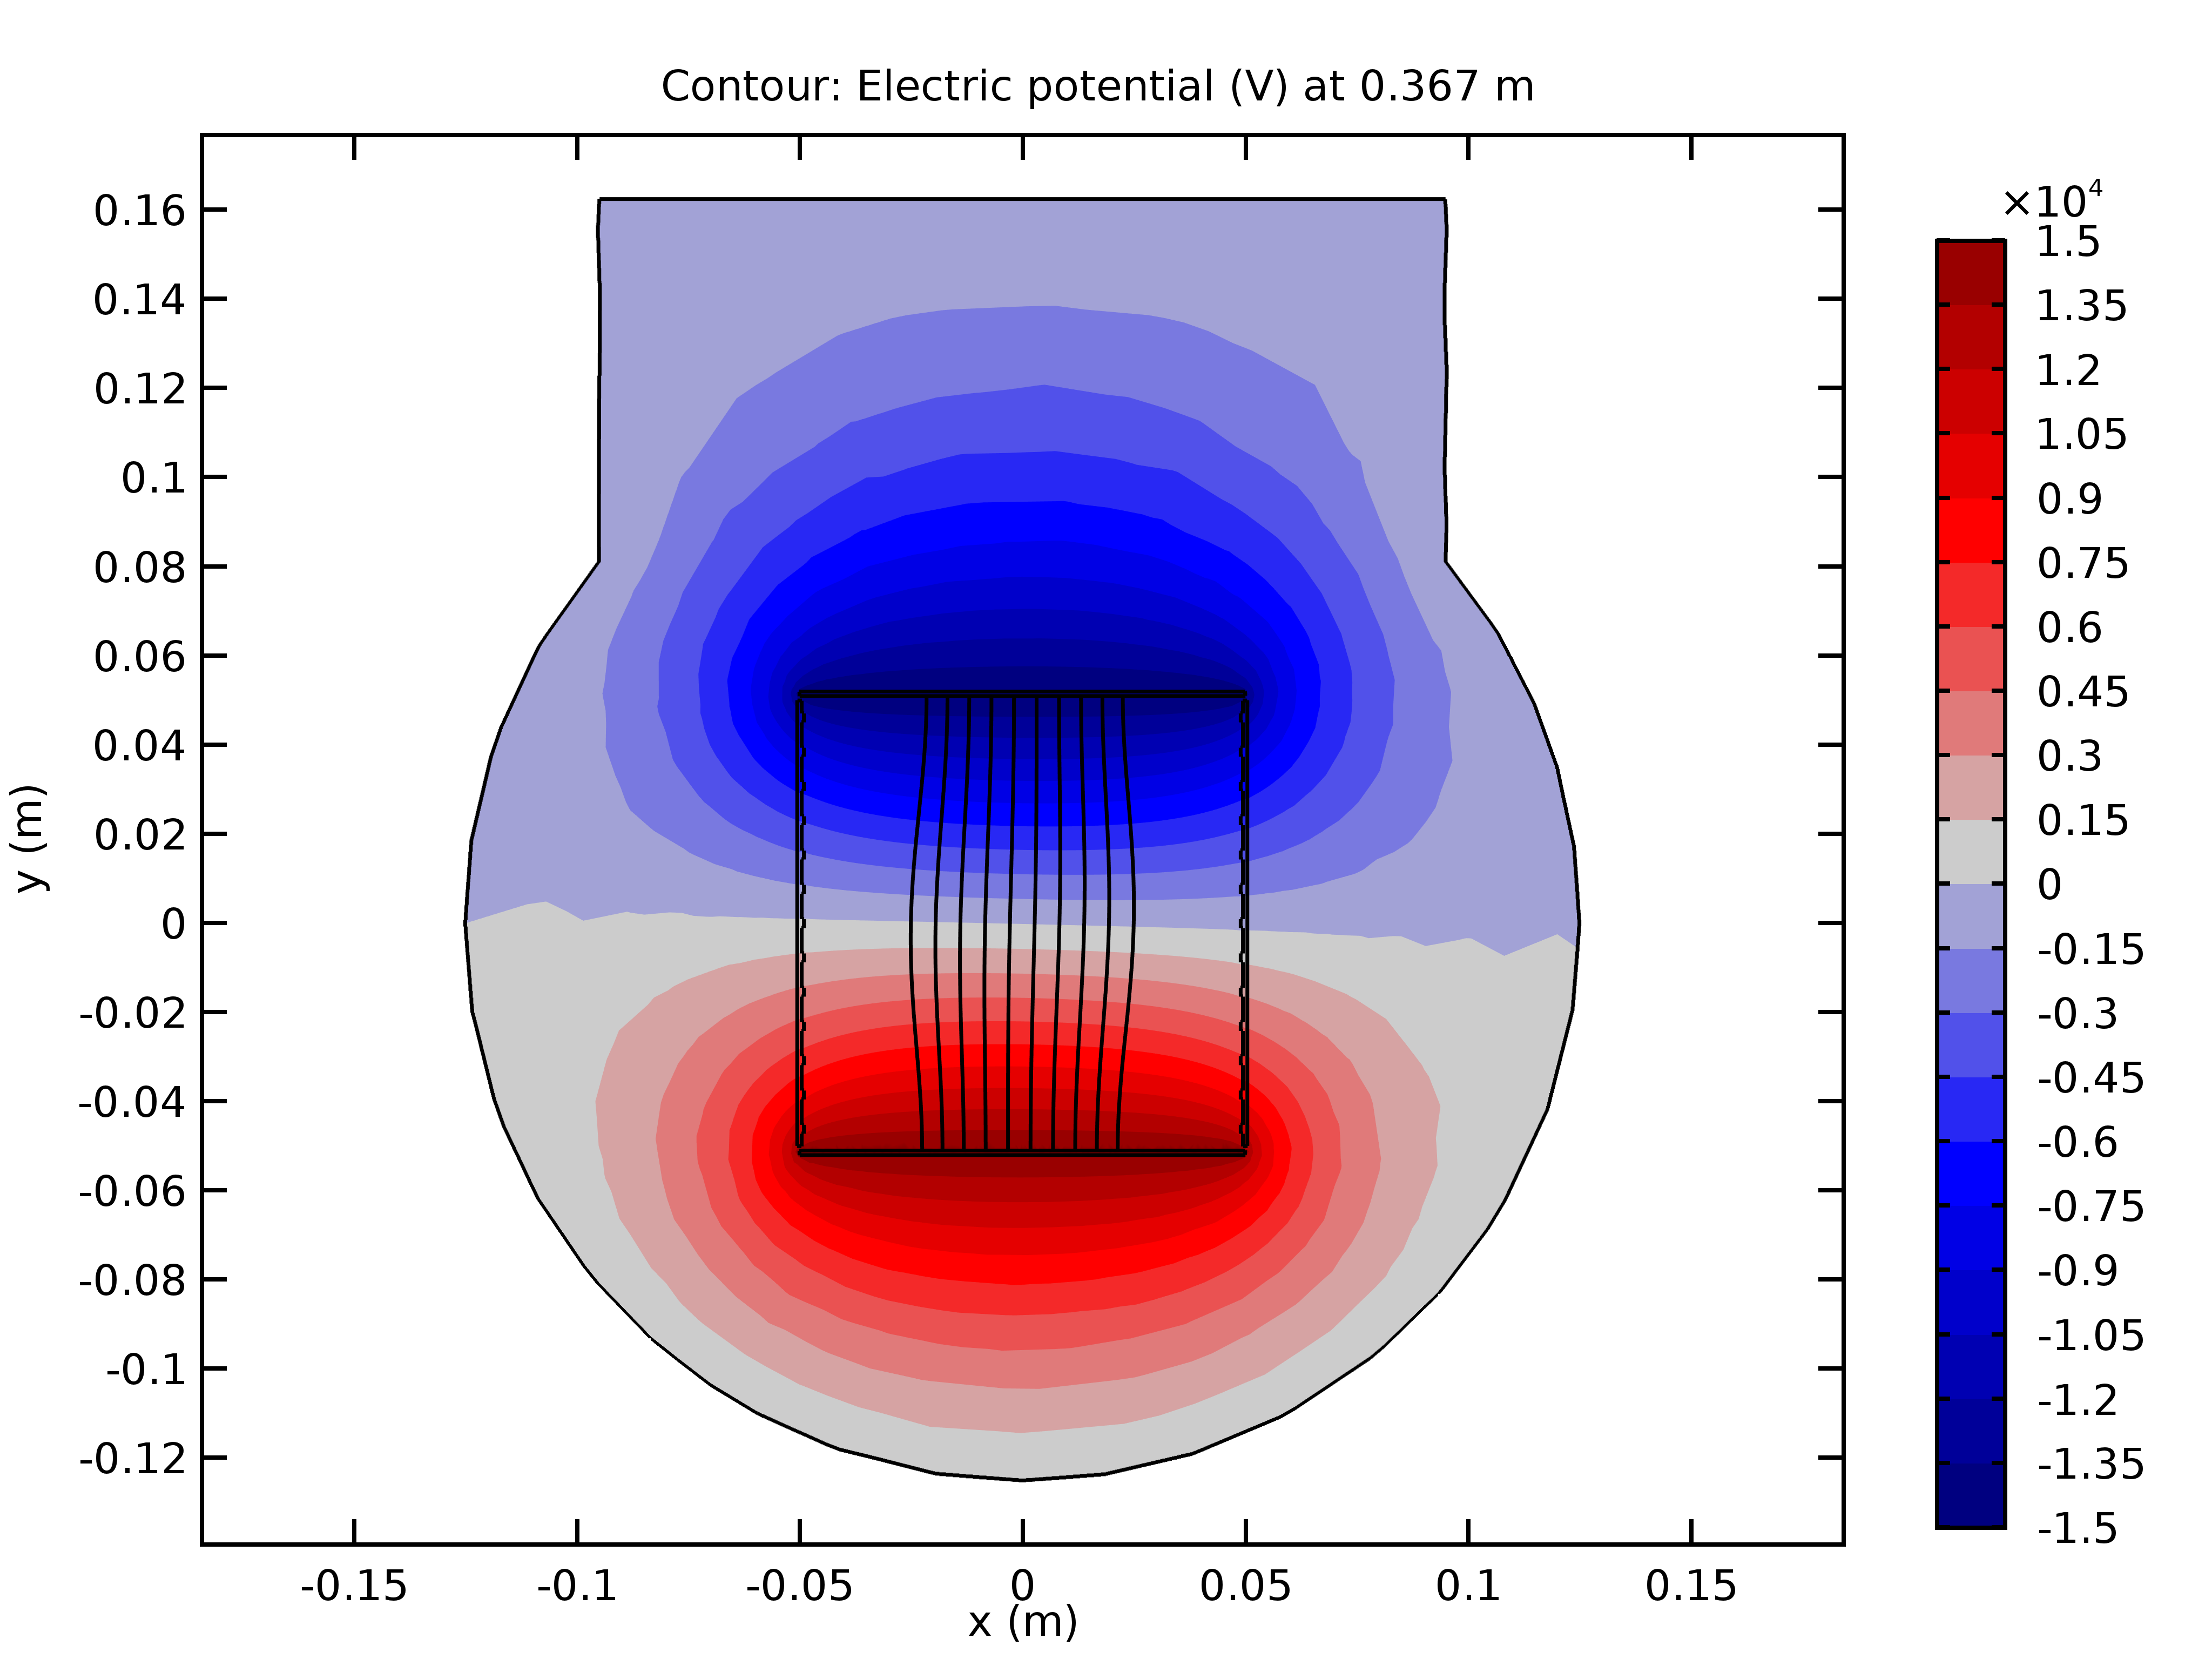
\includegraphics[width=\textwidth]{03_Prototype/figures/fig021_image_asym_sym_b.png}
		\caption{Symmetric configuration.}
		\label{chap3:asym_sym_b}
	\end{subfigure}
	~
	\begin{subfigure}{0.5\textwidth}
		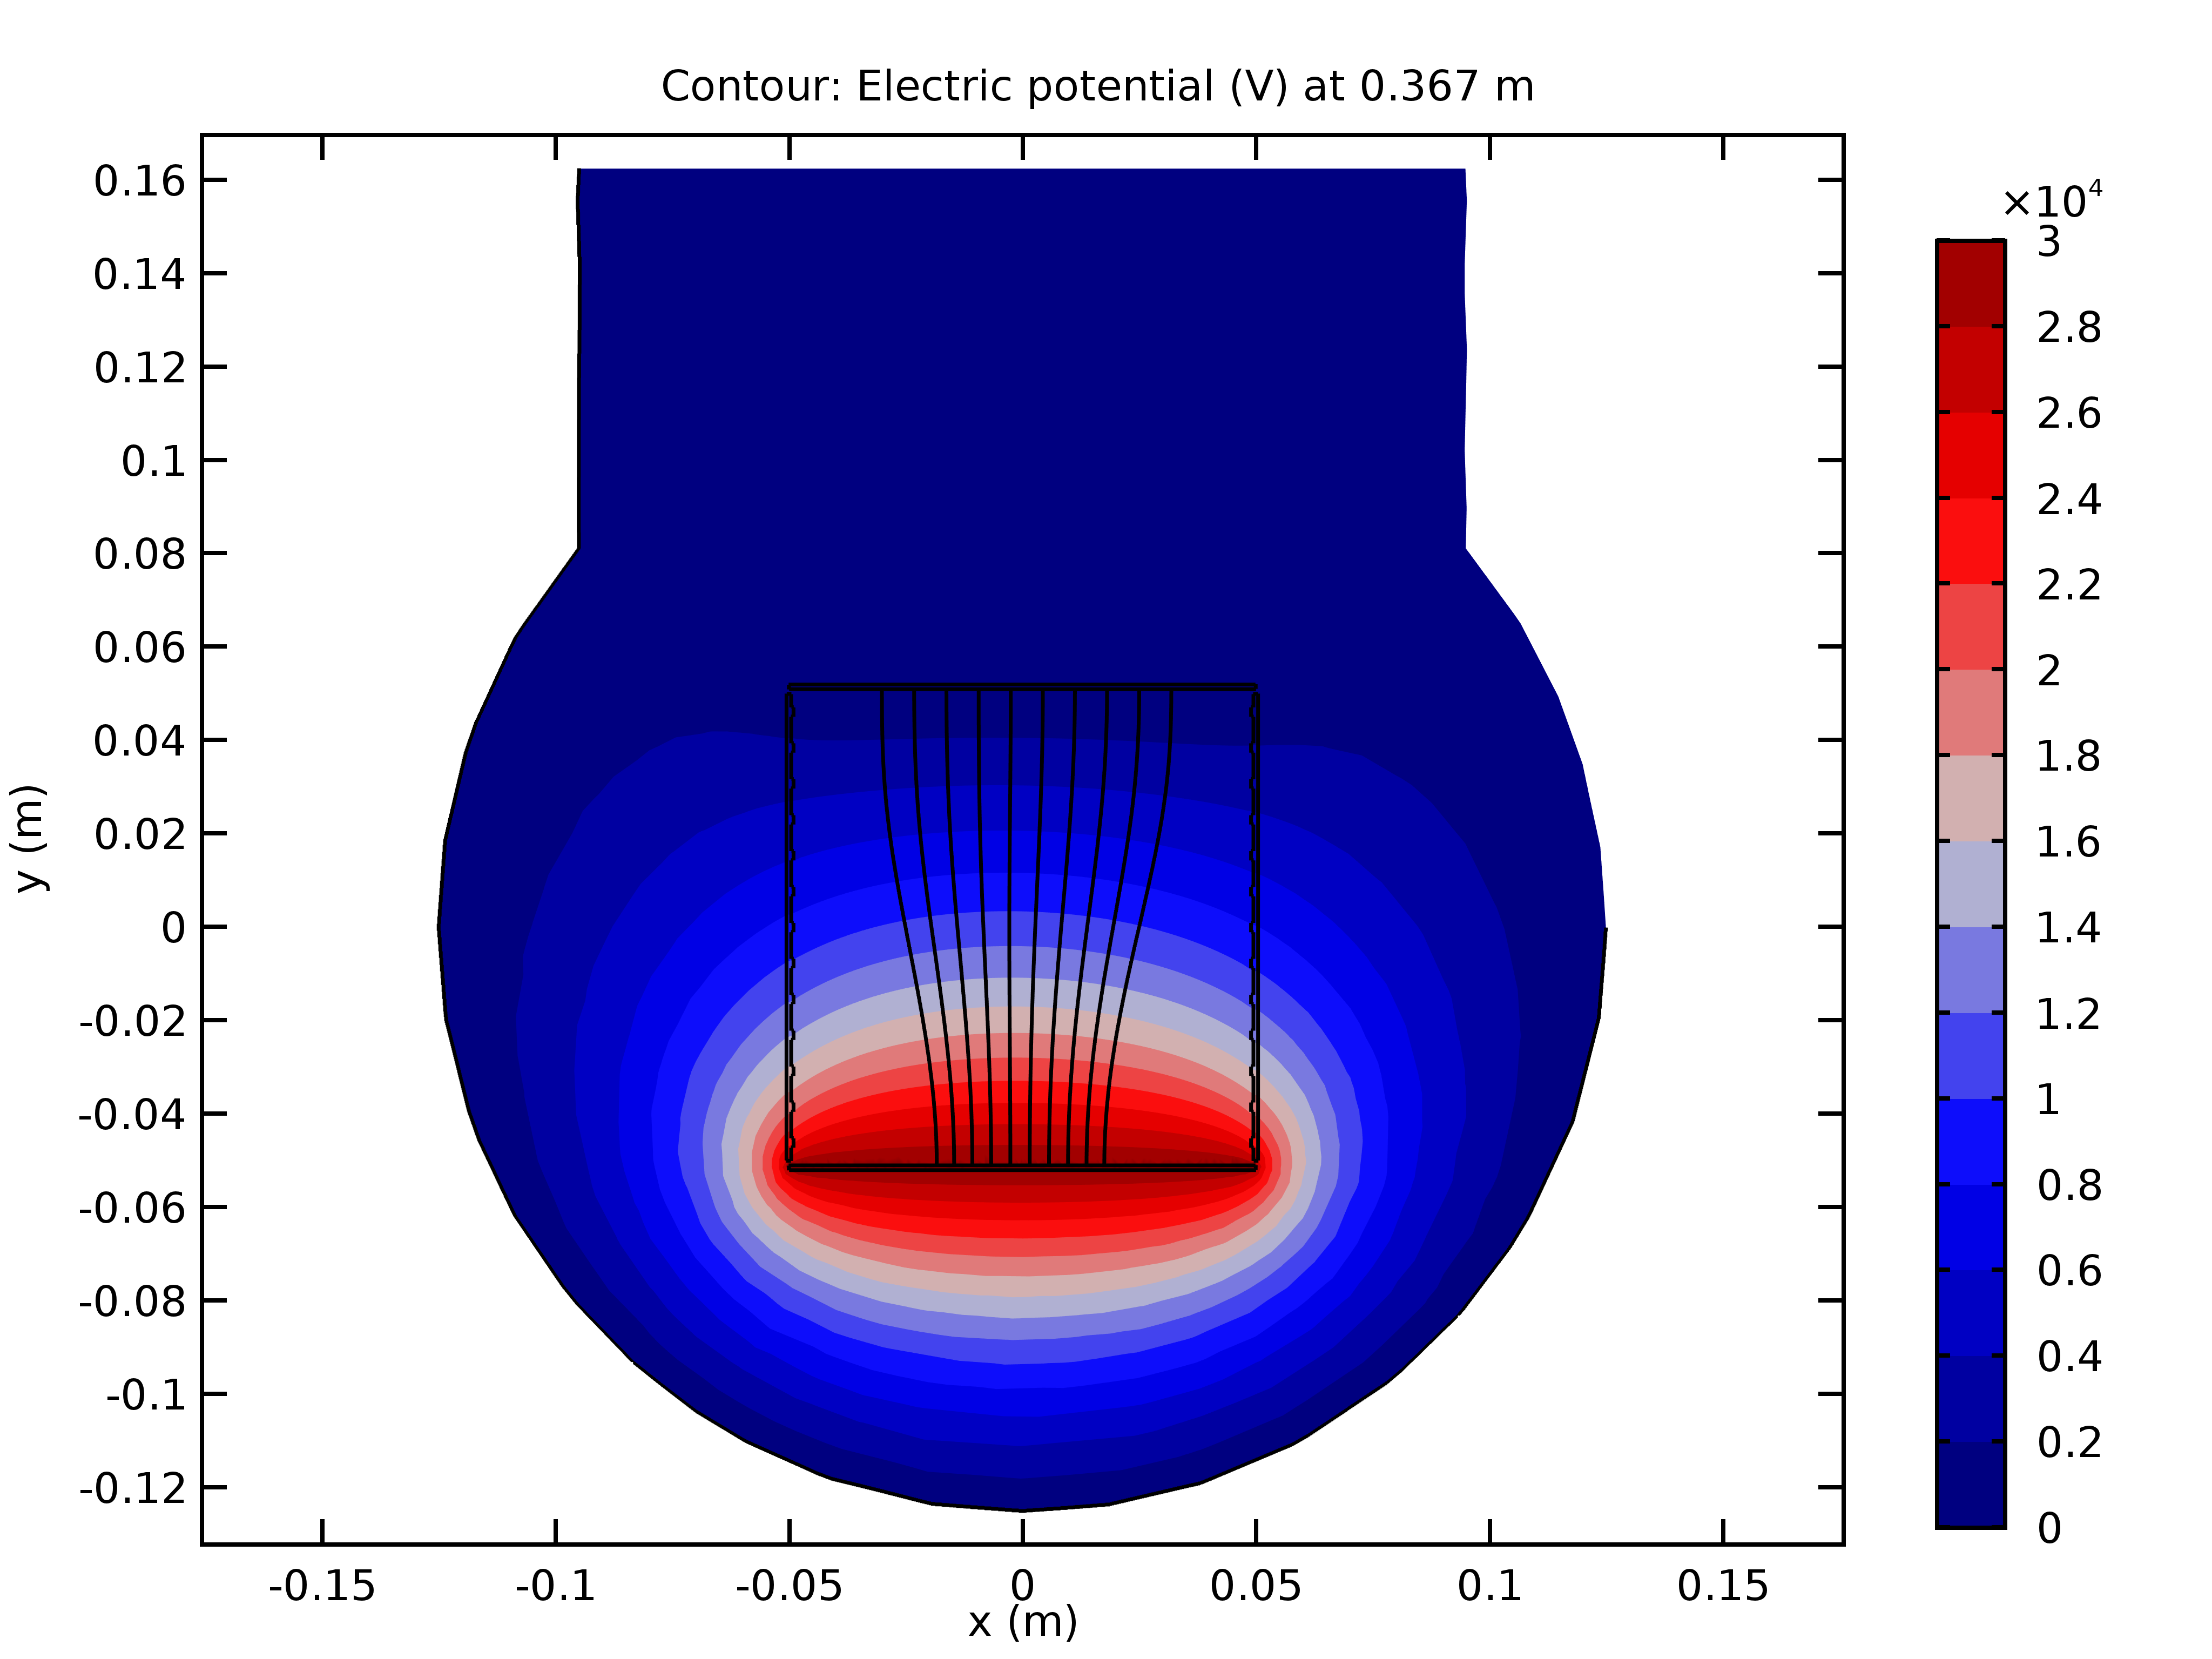
\includegraphics[width=\textwidth]{03_Prototype/figures/fig021_image_asym_sym_a.png}
		\caption{Asymmetric configuration.}
		\label{chap3:asym_sym_a}
	\end{subfigure}
	\caption[Comparison between symmetric and asymmetric configuration]{Comparison between symmetric and asymmetric configuration.}
	\label{chap3:asym_sym}
\end{figure}


  In this configuration (Fig. \ref{chap3:asym_sym_b}), the field focuses the particles in the transverse plane but also in the longitudinal plane. This explains why the particle number on the readout is higher than the expected number. In symmetric, only the transverse plane should be corrected.

  In asymmetric configuration (Fig. \ref{chap3:asym_sym_a}), the field is defocusing in the transverse plane, but also in the  longitudinal one. The projection of the beam will be much broader than expected and many particles are lost during the particle drifts. Therefore, the electric field must be improved in both planes.


  \subsection{IPM cross-interaction [B]}

  The IPMs are in close proximity in order to measure the beam profile in the two transverse  directions. This proximity leads to a coupling effect between the two IPMs due to fringe fields. Moreover, the uniformity of the electric field is strongly related to the geometry that encloses the IPMs. The LWU walls are at ground potential, hence the uniformity of the electric field in the IPMs depends on their position in the LWU. This means that the electric field in each IPM has to be corrected individually.

  We simulated in COMSOL different IPM configurations with and without disks separating the IPMs and located in different positions. The IPMs cannot be shifted too much at the interior of the vacuum vessel because the space is limited by the WS on the left and by the LWU walls on the right. So, we found out that it is much easier to use disks. Fig. \ref{chap3:IPM_disk} shows the influence of disk on the electrical field.

  \begin{figure}[!ht]
	\centering
	\begin{subfigure}{0.7\textwidth}
		\includesvg[width=\textwidth]{03_Prototype/figures/fig022_2IPM_ASYM_NODISK_NODEG_a}
		\caption[]{Electrical field without disk.}
		\label{chap3:no_disk}
	\end{subfigure}

	\begin{subfigure}{0.7\textwidth}
		\centering
		\includesvg[width=\textwidth]{03_Prototype/figures/fig022_2IPM_ASYM_DISK_NODEG_c}
		\caption{Electrical field with disks.}
		\label{chap3:disks}
	\end{subfigure}
	\caption[Influence of shielding disks on the IPM electric field]{Influence of shielding disks on the IPM electric field along the LWU.}
	\label{chap3:IPM_disk}
\end{figure}


  The quadratic mean is plotted for each electrical component in the middle of the IPM, as described in section \ref{}. A field overlap occurs when no disk is mounted between the two IPMs. When disks are present, the fields are constrained within the space in-between two disks and the cross interaction effect is less important. On the other hand, the field variations are sharper in this area, so the longitudinal field component is worse with disks. One can see that the field shape is the same in both IPMs because they are independent of the LWU geometry. This is quite useful because the same corrections can be applied to the two IPMs and it simplifies the optimization of field correctors.

  \subsection{Field corrections [B]}
  \label{chap3:field_corrections}
  \begin{wrapfigure}{r}{0.45\textwidth}
	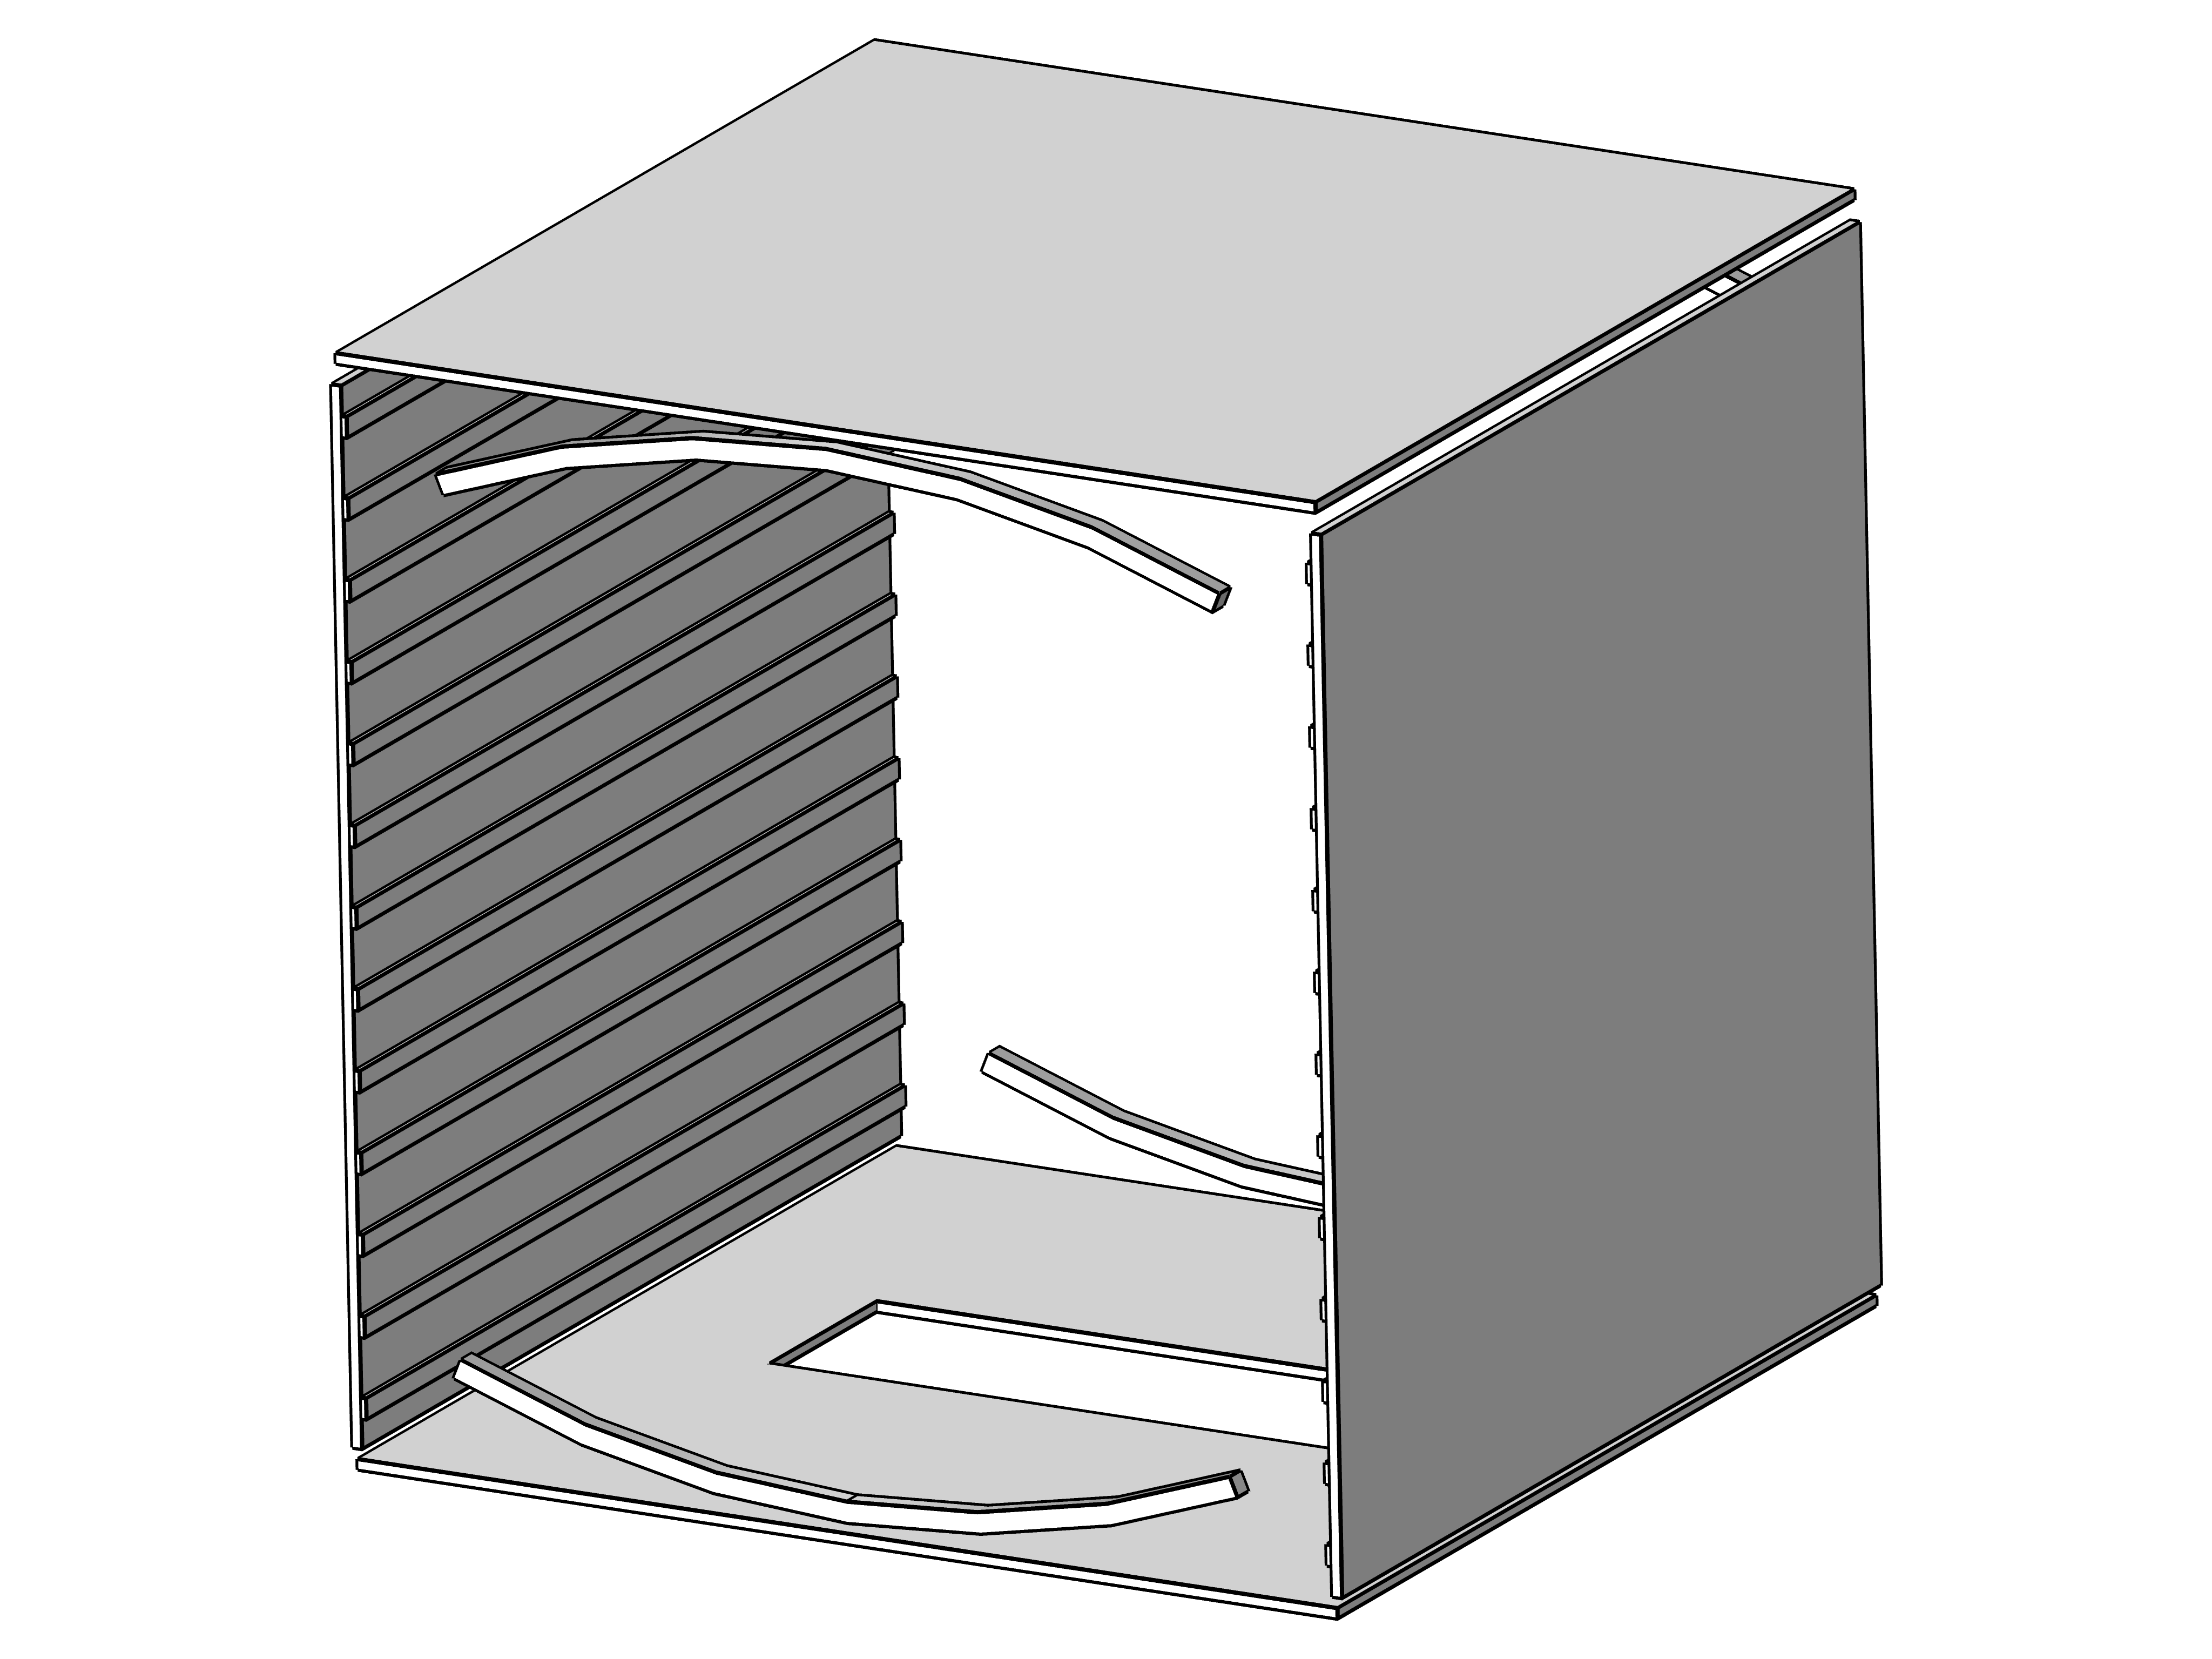
\includegraphics[width=0.45\textwidth]{03_Prototype/figures/fig026_IPM_COMSOL.png}
	\caption[IPM geometry in COMSOL]{IPM geometry in COMSOL.}
	\label{chap3:IPM_COMSOL}
\end{wrapfigure}

  The electric field is improved by means of field correctors (also called field degraders) and curved electrodes. Fig. \ref{chap3:IPM_COMSOL} shows the COMSOL geometry of an example of IPM that has been simulated. One can see the degraders on each side and the curved electrodes at the top and bottom of each IPM.

  The field correctors will constrain the electric potential at a certain value on the side of the IPM. Thus, the iso-potential will be more flat in the IPM, so the field will be more uniform. In practice, field degraders are just conductive pieces connected to a voltage source. One can directly connect them to power supplies. This method allows to tune finely the potential on the electrodes.
  On the other hand, it requires HV feedthroughs for each electric potential. Unfortunately, we cannot implement this solution since the available space on the IPM flange is restricted. We will instead exploit directly the existing high voltages to feed a resistor bridge as shown in Fig. \ref{chap3:resistor_chain}. The potential at each field corrector is simply given by the Ohm law:
  \begin{equation}
    V_{i} = \frac{\sum_{k = 1}^{i} R_{k}}{\sum_{j = 1}^{N} R_{j}}V_{HV} \label{chap3:PontDiviseur}
  \end{equation}

  \begin{wrapfigure}{l}{0.3\textwidth}
	\begin{center}
		\begin{tikzpicture}[scale=0.8,transform shape,american voltages]
			\draw (0,0) node[label={above:HV}] {} to [short, *-] (2,0)
			to [R, l_=$R_1$] (2,2)
			to [R, l_=$R_2$, *-] (2,4);
			\draw (0, 9) node[label={above:HV}] {} to [short, *-] (2,9)
			to [R, l_=$R_{N}$] (2,7)
			to [R, l_=$R_{N-1}$, *-] (2,5)
			(2,4.5) node[] {...};
		\end{tikzpicture}
	\end{center}
	\caption[Resistor chain]{Resistor chain.}
	\label{chap3:resistor_chain}
\end{wrapfigure}


  This method has anyhow some drawbacks. The choice of resistor is limited, since not all resistance values are not available commercially \cite{Vishay2012}. Thus, not all possible corrections are not available. In addition, the use of resistor in a vacuum is not really recommended since it often requires welding. Also, the resistors should be capable to stand  high activity levels, mainly considering that, if one of them is damaged the entire bridge is affected.

  We decided to use $13$ degraders, regularly spaced by $7.5\,\mathrm{mm}$ from each other, on each side of the IPM. A degrader is $2\,\mathrm{mm}$ width and $100\,\mathrm{mm}$ long (in longitudinal direction). The $7^{th}$ degrader is located in the middle plane of the IPM.

  The electric potential value which gives the best uniformity is computed with COMSOL for each degrader. The resistor chain is determined from these values with respect to the equation (\ref{chap3:PontDiviseur}). For each corrector, two commercial off-the-shelf (COTS) resistors are mounted in series allowing values as close as possible to the optimal one. Resistors are selected within the $\mathrm{M\Omega}$ range, reducing the power consumption of power supplies. The field simulation is recomputed with the real resistors and potential values.

  In the case of the symmetrical IPM, only the first $6$ degraders must be calculated since the $7^{th}$ is grounded and the last $6$ potentials are held at opposite potentials with respect to  the first 6 ones, due to symmetry. The voltage and resistor values of the degrader chain for symmetric IPM are tabulated in the Table \ref{chap3:resistor_sym}.

  \begin{table}[ht]
	\centering
	\caption[Description of the resistor chain for the field degraders in the symmetric IPM]
	{Description of the resistor chain for the field degraders in the symmetric IPM.}
	\label{chap3:resistor_sym}
	\begin{tabular}{lllllllll}
		\toprule
		                                & 1  & 2     & 3      & 4    & 5      & 6     & 7    &    \\
		\midrule
		%Voltage (\(\mathrm{kV}\))       & 15 & 13.57 & 11.32  & 8.72  & 6.52   & 4.31  & 2.16 & 0  \\
		%Resistor (\(\mathrm{M}\Omega\)) &    & 13.24 & 20.83  & 24.07 & 20.37  & 20.46 & 19.9 & 20 \\
		Resistor (\(\mathrm{M}\Omega\)) &    & 13.4  & 20.715 & 24.3 & 20.332 & 20.51 & 20   & 20 \\
		Voltage (\(\mathrm{kV}\))       & 15 & 13.56 & 11.32  & 8.71 & 6.52   & 4.31  & 2.15 & 0  \\
		\bottomrule
	\end{tabular}
\end{table}

  A particle tracking was performed with the real corrected field and the results are shown in Fig. \ref{chap3:SymTransversalProfile}. One sees that, even without correction, the symmetrical IPM gives fairly good results. The focusing effect, shown in the previous section, is visible and explains why there are more particles on readout than expected. When the field correctors are enabled, the profile is extremely well reconstructed with an error of less than $0.2\,\mathrm{\%}$.  This fulfills the requirements of ESS on the profile error.

  \begin{figure}[!h]
	\begin{center}
		\includesvg[width=\textwidth]{03_Prototype/figures/fig023_SymTransversalProfile}
	\end{center}
	\caption[Particle tracking for real symmetric field configuration with and without configuration]{Particle tracking for real symmetric field configuration with and without configuration (degraders and disks). Beam is assumed to be gaussian with a size $\sigma_{beam}=3\,\mathrm{mm}$ [Image à refaire]}
	\label{chap3:SymTransversalProfile}
\end{figure}


  For the asymmetric IPM, we proceeded in the same way. Also in this case, the resistor chain had to be optimized as well as the two curved electrodes. Table \ref{chap3:resistor_asym} gives the values of resistances and potentials in the case of the asymmetric IPM.

  \begin{table}[ht]
  \noindent
  \caption[Description of the resistor chain for the field degraders and curved electrodes in the asymmetric IPM]
  {Description of the resistor chain for the field degraders and curved electrodes in the asymmetric IPM. [A finir je dois remplir avec les bonnes valeurs]}
  \label{chap3:resistor_asym}
  \begin{tabular}{llllllllll}
    \toprule
                                    & Curved &      & HT    &      & 1     &      & 2    &      & 3    \\
    \midrule
    Resistor (\(\mathrm{M}\Omega\)) &        & 20.5 &       & 17.2 &       & 15.5 &      & 22.2        \\
    Voltage (\(\mathrm{kV}\))       & 30     &      & 27.63 &      & 25.64 &      & 23.85 &      & 21.29 \\
    \bottomrule
  \end{tabular}
  \\
  \medskip
  \begin{tabular}{lllllllllll}
    \toprule
                           &      & 4  &      & 5  &    & 6  &      & 7  &      & 8  \\
    \midrule
    Resistor (\(\mathrm{M}\Omega\)) & 24.1 &    & 19.5 &    & 20 &    & 19.5 &    & 13.5      \\
    Voltage (\(\mathrm{kV}\))       &      & 18.5 &      & 16.25 &    & 13.94 &      & 11.69 &      & 10.13 \\
    \bottomrule
  \end{tabular}
  \\
  \medskip
  \begin{tabular}{lllllllllll}
    \toprule
                           &    & 9  &      & 10 &      & 11 &       & 12 &      & 13 \\
    \midrule
    Resistor (\(\mathrm{M}\Omega\)) & 16 &    & 17.2 &    & 13.4 &    & 18.51 &    & 13.5      \\
    Voltage (\(\mathrm{kV}\))       &    & 8.28 &      & 6.3 &      & 4.74 &       & 2.6 &      & 1.05 \\
    \bottomrule
  \end{tabular}
  \\
  \medskip
  \begin{tabular}{llll}
    \toprule
                           &     & Gnd & Curved \\
    \midrule
    Resistor (\(\mathrm{M}\Omega\)) & 9.1 &     &        \\
    Voltage (\(\mathrm{kV}\))       &     & 0  & 2850      \\
    \bottomrule
  \end{tabular}

\end{table}

  The results of the particle tracking, for the asymmetric case, are shown in Fig. \ref{chap3:AsymTransversalProfile}. The asymmetric field defocuses particles in both directions when the correctors are missing. So the reconstructed profile is $35\,\mathrm{\%}$ wider and some particles do not even reach the readout. The shift in position is due to the cross interaction between the two IPMs. When corrections are enabled, the obtained transverse profile is much better: the error on the profile is only $0.4\,\mathrm{\%}$. The position is also corrected thank to the shielding disks and curved electrodes, therefore no more shift appears. However, the correction on the longitudinal field is not as good as in the case of symmetric configuration and some particles are still lost during the drift: only $77\,\mathrm{\%}$ of the particles will reach the readout.

  \begin{figure}[!h]
	\begin{center}
		\includesvg[width=\textwidth]{03_Prototype/figures/fig025_AsymTransversalProfile}
	\end{center}
	\caption[Particle tracking for real asymmetric field configuration with and without configuration]{Particle tracking for real asymmetric field configuration with and without configuration (degraders and disks). Beam is assumed to be gaussian with a size $\sigma_{beam}=3\,\mathrm{mm}$.}
	\label{chap3:AsymTransversalProfile}
\end{figure}


  \subsection{Grid [A]}
  \label{chap3:sec:grid}
  As shown in the Fig. \ref{chap3:IPM_COMSOL}, the readout electrode is not completely filled: a rectangular slit allows the ions or electrons to move toward the readout system. This slit is relatively big ($2\times5\,\mathrm{cm^{2}}$) with respect to the electrode dimensions ($10\times10\,\mathrm{cm^{2}}$), so it affects the electric field uniformity. A wire mesh can easily overcome this problem. Indeed in the close proximity of the mesh the field is not very straight, but at further distances the field becomes constant. The mesh allows to have always the same field uniformity in the IPM whatever readout is used. On the other hand, it represents an obstacle for the incident particles, therefore the grid must be choose carefully.

  Actually, many of our colleagues are involved in the development of Micromegas detectors. So we have access to several types of mesh. We started with a stainless steel mesh with a pitch of $450\,\mathrm{\mu m}$ and a wire size of $50\,\mathrm{\mu m}$, so the optical transparency is about $90\,\mathrm{\%}$. The thickness is about $XX\,\mathrm{\mu m}$. A first approximation can be made with the Fourier series of the electric potential as proposed by Feynman \cite{feynman2011feynman}:
  \begin{equation}
    V(x,y)= \sum^{\infty}_{n=0} A_{n} \cdot cos(-\frac{2\pi n x}{\lambda}) \cdot exp(-\frac{2\pi n y}{\lambda})
  \end{equation}

  In this case the grid is regularly spaced in the $x$ direction by a step $\lambda$. If we are at a distance $k \cdot \lambda$ away from the grid the first harmonic is attenuated by a factor $e^{-2\pi k}$. This tendency can be easily confirmed with the FEM or BEM method. Fig. \ref{chap3:Grid} shows the electrical potential close to the mesh for two different field configurations. One can see that the field is almost constant starting from less than $1\,\mathrm{mm}$ distance from the mesh. So there will be no problem using this grid.

  \begin{figure}[!ht]
	\centering
	\begin{subfigure}{\textwidth}
		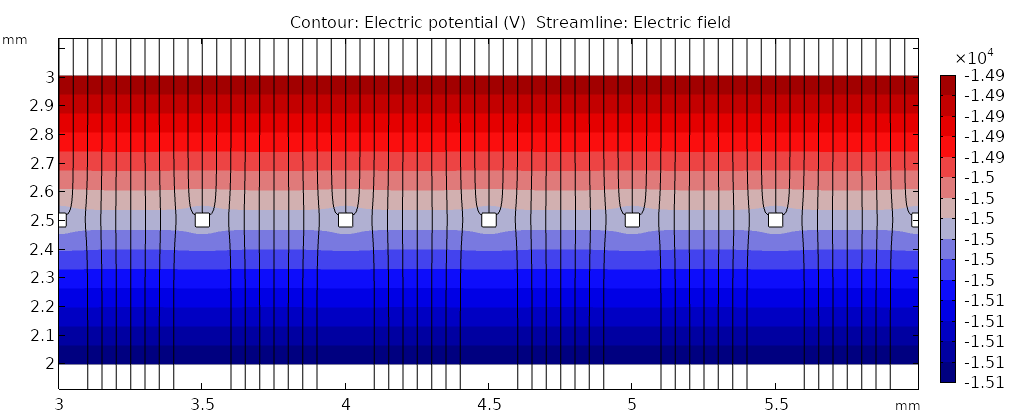
\includegraphics[width=\textwidth]{03_Prototype/figures/fig027_Grid1.png}
		\caption[]{Configuration 1: The field is constant (up: \(3\,\mathrm{kV/cm}\); down: \(3\,\mathrm{kV/cm}\)). The mesh transmission is close to the optical transparency.}
		\label{chap3:Grid1}
	\end{subfigure}

	\begin{subfigure}{\textwidth}
		\centering
		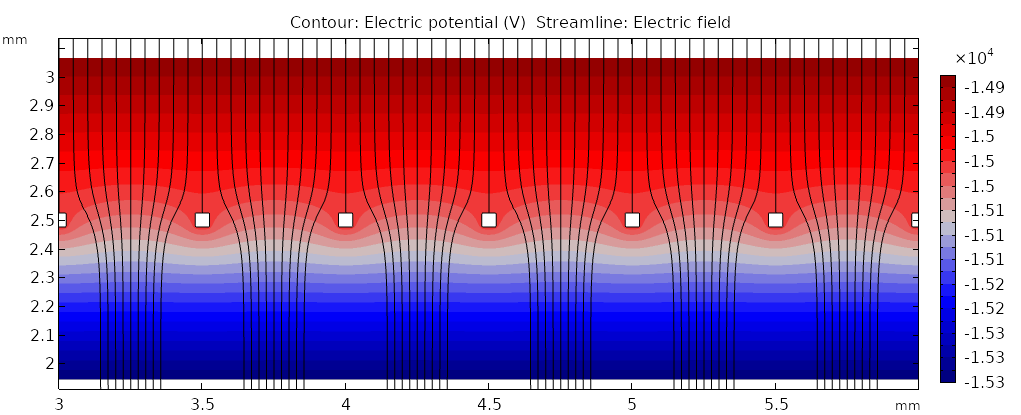
\includegraphics[width=\textwidth]{03_Prototype/figures/fig027_Grid2.png}
		\caption[]{Configuration 1: The field is higher below the grid (up: \(3\,\mathrm{kV/cm}\); down: \(6\,\mathrm{kV/cm}\)). The mesh transmission is higher than the optical transparency.}
		\label{chap3:Grid2}
	\end{subfigure}
	\caption[Electrical simulations of a \(50/450\,\mathrm{\mu m}\) grid]{Electrical simulations of a \(50/450\,\mathrm{\mu m}\) grid. Two different field configurations were simulated. Both shows that the electrical field becomes uniform few mm away from grid. However the particle transmission differs due different ratios of the electric fields imposed in the two regions.}
	\label{chap3:Grid}
\end{figure}


  The grid is an obstacle for the incoming particles, and the number of stopped particles is directly related to the optical transparency of the grid. However it is possible to improve the transmission by increasing the field on one side of the grid. A simple analytical model has been demonstrated in the case of wire grids \cite{Bunemann1949}. We assume that our grid follows this model\footnote{This is not really true since our mesh is not made of cylindric wires.}:
  \begin{equation}
    \frac{E_{r}}{E_{d}} \geq \frac{1+\frac{2 \pi r}{\lambda}}{1-\frac{2 \pi r}{\lambda}}
  \end{equation}
  where $E_{r}$ is the field on the readout region, $E_{d}$ is the field on the drift region and $r$ the wire diameter. For our mesh configuration the ratio $\frac{E_{r}}{E_{d}}$ must be higher than $4.38$.
  An example is given in Fig. \ref{chap3:Grid}. The top figure shows a case where $E_{r}=E_{d}$. The field lines may be stopped by the mesh wires. In the bottom figure, $E_{r}=2 \cdot E_{d}$ and the field lines are attracted into the readout region due to the field difference.

  The grid can be polarized in order to use it as a Frish grid. For some readout, it allows to get rid of certain signal contributions. More details will be given in section \ref{chap3:ramo} of this chapter.

  Finally, the grid may be also used to shield the readouts against possible electromagnetic noises created by all the radio-frequency devices. The effectiveness of the grid is clear. The wavelengths for the two ESS frequencies\footnote{We only considered the first harmonic} are respectively $80\,\mathrm{cm}$ and $40\,\mathrm{cm}$. The pitch of our grid is far less than theses wavelengths.

  %\subsection{Summary}

  \section{Initial momentum [A]}
  So far, we assumed that the ions and/or electrons were created without initial velocity i.e. at rest in a pure electric field. In this case, electrons and ions give same results and the value of the extraction field does not matter. In reality, these particles have a non-negligible initial speed and may be affected by parasitic electromagnetic fields. This can greatly affect the profile, thus the extraction field must be increased in order to minimize such distortion. In the following sections, we will try quantify these effects to determine the nominal value of the extraction field.
  %The second limitation concerns possible \acrshort{hv} breakdowns. In very high vacuum a distance of some millimeter is sufficient to isolate several tens of kilovolts. However, the breakdowns are also strongly influenced by the surface states of the electrodes, the composition of the vacuum and the presence of leakage current \cite{Latham1995}. Hence, we should keep a standoff distance between the electrode and the vacuum vessel (less than 1kV/cm between the IPMs and LWU).

  \subsection{Thermal distribution [A]}
  A first approximation of the initial speed of ions can be done thanks to the distribution of Maxwell-Boltzmann. The distribution of the speeds with respect to the particle mass and the temperature is given by the following equation:

  \begin{equation}
    F(\boldsymbol{v}) = \left(\frac{m_{part}}{2 \pi k_{b} T}\right)^{\frac{3}{2}}\exp\left(-\frac{m_{part}\boldsymbol{v}^{2}}{2 k_{b} T}\right)
  \end{equation}
  % \begin{wrapfigure}{r}{0.5\textwidth}
% 	\includesvg[width=0.5\textwidth]{03_Prototype/figures/fig013_maxwell_gas2}
% 	\caption[Maxwell-Boltzmann distribution for some species of ESS residual gas]{Maxwell-Boltzmann distribution for some species of ESS residual gas.}
% 	\label{chap3:maxwell_gas}
% \end{wrapfigure}
\begin{figure}[!ht]
	\centering
	\includesvg[width=0.7\textwidth]{03_Prototype/figures/fig013_maxwell_gas2}
	\caption[Maxwell-Boltzmann distribution for some species of ESS residual gas]{Maxwell-Boltzmann distribution for some species of ESS residual gas.}
	\label{chap3:maxwell_gas}
\end{figure}
  Where, $k_{b}$ is the Boltzmann constant, $T$ the temperature, $\boldsymbol{v}$ is the speed vector of the considered particle and $m_{part}$ its mass. The Maxwell-Boltzmann distribution works well for perfect gases at low densities. We assumed that is true for the ESS residual gas. The speed is uniformly distributed along all direction ($4\pi$).

  The Fig. \ref{chap3:maxwell_gas} shows the normalized distributions for some of the molecules present in the ESS residual gas. One can see directly that the speed of the fastest ion is below $5000\,\mathrm{m/s}$. A field of few hundred volts per centimeter is more than enough to compensate this effect. It gives no significant difference during the particle tracking. So, we can completely neglect the thermal motion for ions.

  \subsection{Ionization energy distribution [En cours de rédaction]}
  Garfield++ can be used again to quantify the initial energy of the ionization electrons. Indeed Garfield++ gives the energy spectrum of the electrons created by ionization and the directions of emission. Fig. \ref{chap3:garfieldangle} exposes the energy spectrum of ionization electrons and the latitude angle distribution for several energies of incident protons. The energy follows a Landau-like distribution with some Auger electrons. The latitude angle is calculated with respect to the direction of the beam and the longitude with the transverse plane. A large proportion of electrons are ejected perpendicular to the direction of propagation whereas the longitudinal angle is uniformly distributed over $2 \pi$.
  
  \begin{figure}[!ht]
	\begin{subfigure}{0.5\textwidth}
		\includesvg[width=\textwidth]{03_Prototype/figures/fig028_garfield_energy.svg}
		\caption{Electron energy distribution.}
		\label{}
	\end{subfigure}
	~
	\begin{subfigure}{0.5\textwidth}
		\includesvg[width=\textwidth]{03_Prototype/figures/fig028_garfieldangle_2.svg}
		\caption{Electron emission angle distribution}
		\label{}
	\end{subfigure}
	\caption[Energy and emission angle of the ionized electrons]{Energy and emission angle of the ionized electrons.}
	\label{chap3:garfieldangle}
\end{figure}


  \section{Space charge effect [En cours de rédaction]}
  \subsection{Lorentz transformation of electromagnetic fields [En cours de rédaction]}
  \subsection{ESS/CEA Space Charge algorithm [En cours de rédaction]}
  \subsection{Results/Comparisons/??? [En cours de rédaction]}
  \section{Readout systems [C]}
  The information about the ionized particles that reach the readout is well known thanks to all the previous simulations. However, the readout system has not been defined yet. The main requirements on the readout are the following:
  \begin{itemize}
    \item The system must be sensitive enough to detect small amount of positive or negative charges as calculated in the section \ref{chap3:calc}.
    \item It should be compliant with the high vacuum and ISO-5 environnement.
    \item The readout should be able to work in a radiative environnement. 
    \item The reliability of the devices should be high limiting the maintenance actions. 
  \end{itemize}

  The conductive strip detection is the most robust solution, but its sensibility is limited. When signal is too low, it must be amplified. For instance, this can be donne with an Micro Channel Plates (MCP). Semiconductor detectors are also interesting, since they are highly sensitive. This novel method is developed by CERN and shows promising results.
  
  In this section the operating principle of each method is described as well as their advantages and drawbacks.

  \subsection{Ramo-Shockley theorem [A]}
  \label{chap3:ramo}
  In particle detectors the signal is due to the motion of charges within the detector rather than the direct collection of charge by the electrodes. This theorem has been independently demonstrated by Ramo and Schockley \cite{Ramo_1939,Shockley_1938}. The total charge induced on an electrode at a time $t$ by a charged particle $q$ can be easily determined if the particle velocity $\boldsymbol{v}$ and the weighting field $\boldsymbol{E}_{w}$ of the electrode are known:
  \begin{equation}
    i_{n}= q\boldsymbol{v} \cdot \boldsymbol{E}_{wn}
  \end{equation}
  The weighting field is virtual field calculated as follow. All charge are removed, the electrode of interest is set at 1 V while the other electrodes are at ground. This field therefore strongly depends on the electrode and detector geometry.

  Note that if two particles have the same trajectories but opposite charges, the signal will be cancel. In practice, ions and electrons go in two opposite directions in an constant electric field, so the signal adds up. However the electron is much faster, thus it create a very fast signal while the ion signal is more spread in time.

  In general to get rid of one of the components of the next signal that we want to detect ions or electrons. This is done using a so-called Frish grid, placed at a slightly different potential with respect to the reading electrodes. This grid confines the weighting fields in a restricted area and only the particles reaching this zone will induce signal. The grid must have a good transmission (as seen in section \ref{chap3:sec:grid}) it inefficiency remains low as possible \cite{Khriachkov1997,Gook2012}.


  %So if we know the trajectory of the particle it is possible to calculate the current on the electrode at each time.

  %\cite[]{Jen1941}
  \subsection{Strips based detection [En cours de rédaction]}
  Conductive strips is the simplest method to implement. Electrodes are etched on a PCB with a thin layer of copper. Strips a radiation hard
  
  This method is a direct application of Ramo-Schockley's theorem: each strip has its own sensitivity field that depends mainly on its width and its pitch with respect to the other electrodes. The signal contribution of ions or electrons can be computed for each electrodes.

  The performances of this method depend on the reading electronics. In an ideal world, a transimpedance amplifier is sufficient. It converts and amplifies the induced current into voltage, then the voltage is digitized by an ADC. The gain of a transimpedance is proportional to the value of the feedback resistance.

  The reality is much more complex since the electronic elements are not perfect. First, the sensor has a parasitic capacitance and resistance, as well as every components in the analog chain. Nuclear detectors have non negligible impedance that reduce the gain stability of transimpedances.
  For low signal, the feedback resistance must be high enough, but the Johnson’s (or thermal) noise increase linearly with the resistance. At some point, the signal to noise ratio will be too low, so the signal may be not recovered.

  The charge amplifier is more popular for nuclear detector. In this configuration, a capacitor is added in the feedback loop. It compensates the sensor capacitance and allows stable and high gain, but the bandwidth is smaller. A resistor or a switch can be put in parallel to the feedback capacitor allowing the discharge the capacitor.

  Note that amplifiers have their own characteristics that will also limit the bandwidth and gain regardless of the amplifier configuration.

  \begin{figure}[!ht]
  \begin{center}
    \begin{tikzpicture}[scale=1,transform shape,american voltages]
      % Sensor + Cable
      \draw
      (0,0) to[isource, l_=$s$](0,3)
      to[short, -, f=$i_s(t)$] (1.5,3)
      to[C=$C_s$] (1.5,0) -- (0,0);
      \draw 
      (1.5,3) -- (3,3) to[R=$R_s$] (3,0) node[ground] {} to[short] (1.5,0);
      \draw 
      (3,3) -- (4.2,3) to[L=$L_c$] (5.2,3) to [R=$R_c$] (7.2,3) to [C,l_=$C_c$] (7.2,0) to[short] (3,0);
      
      % OPA
      \draw
      (10,2) node[op amp] (opamp) {}
      (opamp.-) |- ($(opamp.-)+(0.2,1)$) to[R=$R_f$] ($(opamp.-)+(2.2,1)$) -|
      (opamp.out)
      (opamp.-) |- ($(opamp.-)+(0.2,2.5)$) to[C=$C_{f}$] ($(opamp.-)+(2.2,2.5)$) -|
      (opamp.out)
      to[short] ($(opamp.out)+(.5,0)$) node [right] {$V_{out}$} node [ocirc] {} (opamp.+) to[short]  ($(opamp.+)-(0,.5)$) node[ground] {} (opamp.-) to[short] ($(opamp.-)-(0,0)$) |- (7.2,3);

      % Rectangle
      \draw[red, thick] (-0.5, -1) rectangle(3.9,4.)
      node[above,xshift=-2cm]{Sensor};
      \draw[blue, thick] (4.1, -1) rectangle(8.,4.)
      node[above,xshift=-2cm]{Cable};

    \end{tikzpicture}
  \end{center}
  \caption[Typical circuit of a charge amplifier with an operational amplifier]{Typical circuit of a charge amplifier with an operational amplifier. The $R_{f}$ and $C_{f}$ should chosen according to sensor characteristics. Strips sensors have low resistance but non negligible capacitance. Usually, cables are modelized by succession of LRC cells, for convenience just one cell is drawn here.}
  \label{chap3:AOPcharge}
\end{figure}


  [Faut-il plus détailler la partie électronique ? Equation ? Fonction de transfert ? Diagramme bode ?]

  Strip detection can not be used when the signal is too low with respect to the electronics, and it is necessary to find a way to amplify the ionization signal.

  \subsection{Interaction of particles with low energies [C]}
  \label{chap3:low_energy}
  In general, a amplification medium is used to increase the signal. In this medium, a primary particle will create many secondary particles. These secondaries will induce an higher signal on the reading electronic. This is the operating principle of gaseous and solid state detectors. Two solid state detector technologies have been forseen since the use of gas detectors is not possible here.

  We should ensure that the detection of low energy ions or electrons is possible for these detectors. The models based on the Bethe equation, presented in the section \ref{chap3:sec_particle_in_matter}, are not precise for these energies and more specific models must be used. Unfortunately, we can not explain and describe these models here. It is much easier to use existing tools for estimating the interaction of particles at low energies. These usually rely on the Monte Carlo methods and we used two different ones.

  SRIM software simulates the interaction of heavy charged particles in matter \cite{srim2013}. The user defines different layers of compounds and the properties of the incident particle in a graphical interface. Then, SRIM computes, among others, the energy depositions, the stopping range, atomic displacements, atom vacancies in the layers.

  Geant4 is a software toolkit that simulates the interaction of particle in a detector \cite{Allison2006, Allison2016}. It is a popular tool for simulating detectors of nuclear or high energy physics. The user describes a detector geometry and associated materials as well as the characteristic of the primary particles. Then, the user adds physical process that will be used for each particle interaction. In our case three models are particularly interesting: the IRCU73 model (ions) the Livermore model (ions and electrons) and the Penelope model (electrons) \cite{Bimbot73,livermore97, salvat2009}. They describe the electromagnetic interaction of charged particle in matter for low energies. A simulation, that uses the previous model, has been developed from a example provided in Geant4 (TestEM11). The simulation tries to reproduce the principles of SRIM. A cube is cut into different layers and the energy loss in each layer is saved.

  \begin{figure}[!h]
	\begin{subfigure}[t]{.5\textwidth}
		\centering
		\includesvg[width=\textwidth]{03_Prototype/figures/fig004_ion_si_deposit}
		\caption[Energy deposition in a silicon layer for various ions]{Energy deposition in a silicon layer for various ions.}
		\label{chap3:ion_si_deposit}
	\end{subfigure}
	~
	\begin{subfigure}[t]{.5\textwidth}
		\centering
		\includesvg[width=\textwidth]{03_Prototype/figures/fig005_electron_si_deposit}
		\caption[Energy deposition in a silicon layer for electrons]{Energy deposition in a silicon layer for electrons.}
		\label{chap3:electron_si_deposit}
	\end{subfigure}
	\caption[Energy deposition in a silicon layer for ions and electron at low kinetic energyies]{Energy deposition in a silicon layer for ions and electron at low kinetic energyies.}
	\label{chap3:si_deposit}
\end{figure}


  Fig. \ref{chap3:si_deposit} shows the energy deposition for different ions (left) and electrons (right) in a silicon cube. For same energies, the electrons deposit their energies along a higher range compare to the ions. Heavy ions are completely stopped before $200\,\mathrm{nm}$ for energies below $15\,\mathrm{keV}$. We want to remind that heavy ions may represent two-thirds of the expected signal.

  \subsection{Semiconductor based detection  [En cours de rédaction]}
  A semiconductor is a crystalline material that can be conductor or insulator depending on the temperature. In a semiconductor, electrons in the valence band are able to reach the conduction band more easily when the temperature increases. The vacancies created by electron in the valence band are called holes. Some elements in groups III to VI of the periodic table are natural semiconductor. However, the semiconducting capabilities of these materials can be greatly increase by implanting impurities in their crystalline structure. In $p$-doping the hole concentration increase whereas $n$-doping boosts the free electrons concentration. Under the action of an electric field electrons and holes diffuse into the crystal structure. The propagation speed depends mainly on the mobility of charge carriers.

  The most basic device is the $pn$-junction. An highly doped $p$ and $n$ semiconductor are put together. At the interface the concentrations of each charge carriers have an important gradient. Therefore, the electron moves to the $p$ doped region whereas the holes reach the $n$ doped region, leaving both respectively positive and negative static ions.
  Static ions create a electric field that, at some point, blocks the flows of the electrons and holes, the junction is at equilibrium.
  If a positive potential is applied between $p$ to $n$ region, then . 
  In reverse bias the a negative voltage is applied the depletion region becomes larger with the potential.

  When a charged particle passes through the silicon it deposits its energy and electron/hole pairs are created as described in the section \ref{chap3:sec_particle_in_matter} of this chapter. The charge carriers drift in the semiconductor due to the bias voltage. 
  A signal is induced on electrodes since the Ramo-Shockley theorem is also valid for semiconductors \cite{Cavalleri1971}.
  \begin{equation}
    i(t) =  \boldsymbol{E_{wpixel}} \left( q_{electron} \mu_{electron} \boldsymbol{E_{bias}} + q_{hole} \mu_{hole} \boldsymbol{E_{bias}} \right)
  \end{equation}
  where $\boldsymbol{E_{wpixel}}$ is the weighting field of a pixel pad, $\boldsymbol{E_{bias}}$ is the field due to $V_{bias}$, $\mu$ are the mobilities of the charge carriers and $q$ their charges.
  %The signal comes from both hole and electron motions.
  Table \ref{chap3:semiconductor} lists the properties of common semiconductors used in radiation detection. 

  \begin{table}[!ht]
	\centering
	\caption[]{Properties of common semiconductors \cite{NSM2005,Eisen1996} used as radiation detector. Properties are given at NTP conditions.}
	\label{chap3:semiconductor}
	\begin{tabularx}{\linewidth}{lXXX}
    \toprule
    Property & $Si$ & $Ge$ & $CdTeZn$ \\
    \midrule
    Density ($\mathrm{g/cm^3}$)& $2.33$  & $5.32$ & $5.78$ \\
    $W$ value ($\mathrm{eV}$) & $3.6$ & $2.95$ & $4.64$ \\
    Breakdown ($\mathrm{V/m}$) & $\approx 3\cdot10^5$ & $\approx 10^5$ & $\approx 10^5$\\
    $e^{-}$ mobility ($\mathrm{cm^{2}/V/s}$) & $\leq 1400$ & $\leq 3900$ & $\leq 1100$\\
    $h$ mobility ($\mathrm{cm^{2}/V/s}$) & $\leq 450$ & $\leq 1900$ & $\leq 100$ \\
    Usage & General purpose & $\gamma$-ray & $X$-ray\\
    Cost & Cheap & Expensive & Moderate\\
		\bottomrule
	\end{tabularx}
\end{table}


  In monolithic sensors, the detection function and the electronic are integrated together in the same substrate. These types of sensors achieve very small dimensions due to the high level of integration. Usually, monolithic sensor are developed for one specific purpose and produced in mass reducing the costs. 

  In hybrid pixel detectors, the two functions are physically separated. The detection matrix is ​​placed on the reading electronics and the connection between the pad and the reading circuits is ensured by bumps. The reading system is independent of the detection matrix making this technology more generic and accessible for small volumes. 

  Semiconductor sensors are very interesting as readout for the IPMs. An electron of $15\,\mathrm{keV}$ deposits all its energy and creates a few thousand electrons/holes pair in silicon. Unlike strips or MCPs the energy of the incident particle is recovered, therefore the signal is more discriminated from possible backgrounds. At last, dead times are short typically in nanosecond range.

  On the other hand, the use of semiconductor with ions at low energies (less $30 \,\mathrm{keV}$) is uncertain. An aluminium coating is often deposited on the top of the sensor to insure a correct polarization. Also first layers of the sensor are not active (dead layers), so the total non sensitive area is around hundred $\mathrm{nm}$. The penetration depth of light ions in silicon is few $\mathrm{nm}$ in the range of $\mathrm{keV}$ as shown in Fig. \ref{chap3:ion_si_deposit}. Therefore, ions create most of the electron/hole pairs in the non sensitive layers.

  Low energetic ions may also produce more damages than electrons in the semiconductor lattice. The creation of charge traps or the change of depletion zones are the worst possible since this may change the signal permanently. Modern semiconductors often implement a pixel calibration circuit to compensate non uniformities.

  \subsection{MCP based detection  [En cours de rédaction]}

  A MicroChannel Plate (MCP) generates electrons from incident particles \cite{Wiza1979}.
  It can be seen as a glass lead plate drilled with micro-metric tilted holes.
  A specific coating is applied on its input surface to increase secondary emissions. When a particle hits the MCP hole entrance then secondary electrons are emitted. Due to difference of potential, secondaries are drawn towards the channel output and strike hole walls again, creating more and more electrons. Then, electrons are collected on a detection plane that can be a single electrode, multiple electrodes or a phosphorus screen depending on the requirements (sensitivity, spatial and time resolution). Fig. \ref{chap3:MCPoutline} presents some schematic representations of how an MCP works.

  \begin{figure}[!ht]
	\begin{center}
		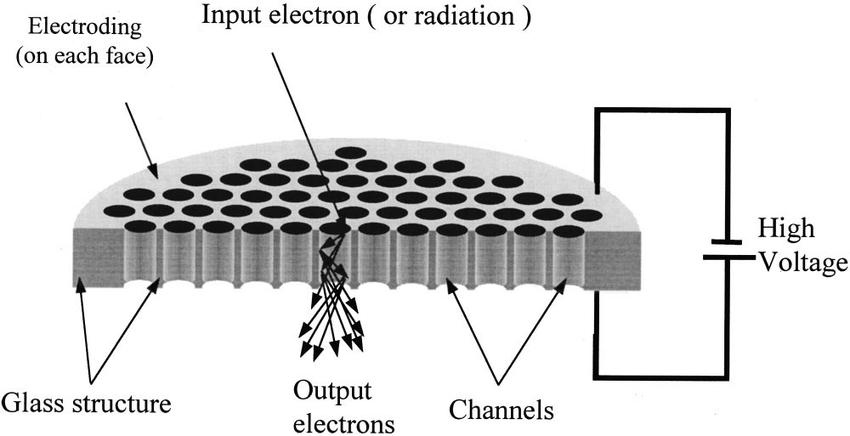
\includegraphics[width=0.7\textwidth]{03_Prototype/figures/fig031_MCP_outline}
	\end{center}
	\caption[]{Sectional view of a MCP \cite{Yi2001}.}
	\label{chap3:MCP_outline_1}
\end{figure}


  \begin{figure}[!ht]
	\begin{subfigure}[t]{0.5\textwidth}
		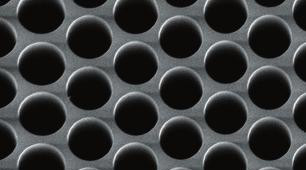
\includegraphics[width=\textwidth]{03_Prototype/figures/fig030_MCPoutline_b2.jpeg}
		\caption[SEM picture of MCP holes]{SEM picture of MCP holes \cite{HamamatsuMCP}.}
		\label{chap3:MCPholes}
	\end{subfigure}
	~
	\begin{subfigure}[t]{0.5\textwidth}
		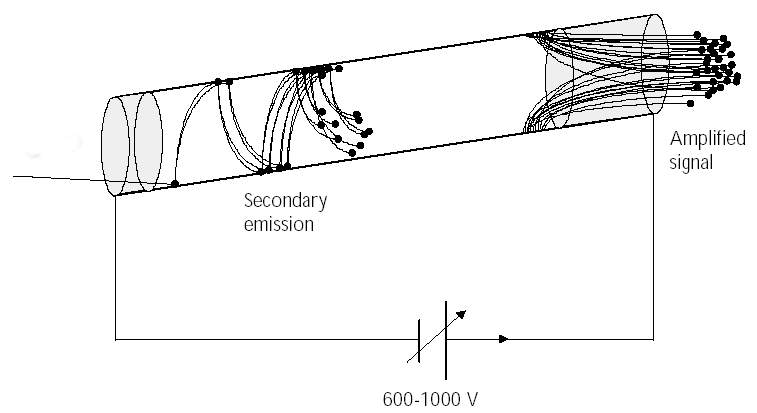
\includegraphics[width=\textwidth]{03_Prototype/figures/fig030_MCPoutline_a.png}
		\caption{Description of how an MCP amplifies incident particle.}
		\label{chap3:MCPchannel}
	\end{subfigure}
	\caption[Schematic views of how a MCP works]{Schematic views of how a MCP works.}
	\label{chap3:MCPoutline}
\end{figure}


  Gain or multiplication factor for a single MCP is about $10^{2}$ to $10^{4}$ depending on the $V_{MCP}$ voltage, usually from $600$ to $1000\,\mathrm{V}$. MCP can be stacked to increase the gain to $10^{6}$ or even more. Typical configurations are single stage, chevron stack (double stages) or Z stack (triple stages).

  Unfortunately MCPs have some drawbacks. First one is the lifetime, indeed the coating is damaged by the incident particles thus the gain is not stable and decreases over the time. Second disadvantage is the MCP gain limitation due to saturation mode. If the incident particle flux is too high then holes may be saturated, and they cannot amplify anymore. When it happens to a channel then it takes some time to recover, generating dead time.

  \section{Background signal [En cours de rédaction]}
  \subsection{Background from beam particles [En cours de rédaction]}
  \subsection{Secondary emission [En cours de rédaction]}

  \section{Summary}
  \label{ch3:Summary}
  This chapter exposed all the studies that have been performed to prove the feasibility of an IPM for the cold part of the ESS accelerator. Three key points were identified: the number of ionization particles, the distortion on the profile and the choice of the readout system.

  The ESS conditions are particularly unfavorable for the ionization cross sections and the high vacuum level in the accelerator does not help. Direct calculations and simulations show that the order of magnitude of the number of ionization particles is about a few thousand particles per pulse per cm for nominal ESS conditions. This number of primary particles seems sufficient to perform a profile measurement assuming that these particles may be detected by the readout.
  
  The non-uniformity of the electric field can be corrected effectively using field correctors and shielding disks regardless of the configuration used. However the symmetrical mode is easier to correct and reduces the maximum voltage required.
  
  The simulations clearly show that the ions are less sensitive to the phenomenon of space charge. The profile measurement with electrons introduces an error that does not satisfy the ESS requirements. It is impossible to install a correction magnet to constrain the trajectories of the electrons. Therefore the measurement of the profile will be done in ions configuration.
  
  The use of ions complicates a the choice of the readout. Strips are an extremely robust method but it requires extremely low noise electronics. MCPs amplify the signal but these devices suffer of aging effect. Silicon detectors are very promising because they are very sensitive, resistant and fast. However, the detection of low energetic ions with these detector is not assured and their implementations are quite complex.

  All of these studies were presented during a Preliminary Design Review which marked the beginning of the construction phase of the different prototypes.
  
  %\begin{figure}[!ht]
	\begin{subfigure}[t]{1.\textwidth}
		\includegraphics[width=\textwidth]{example-image-a}
		\caption[]{}
		\label{}
	\end{subfigure}

	\begin{subfigure}[t]{1.\textwidth}
		\centering
		\includegraphics[width=\textwidth]{example-image-a}
		\caption{}
		\label{}
	\end{subfigure}
	\caption[]{}
	\label{chap:}
\end{figure}

  %\begin{figure}[!ht]
	\begin{subfigure}[t]{0.5\textwidth}
		\includegraphics[width=\textwidth]{example-image-a}
		\caption{}
		\label{}
	\end{subfigure}
	~
	\begin{subfigure}[t]{0.5\textwidth}
		\includegraphics[width=\textwidth]{example-image-a}
		\caption{}
		\label{}
	\end{subfigure}
	\caption[]{}
	\label{chap:}
\end{figure}

  %\begin{figure}[!ht]
	\begin{center}
		\begin{subfigure}{.5\textwidth}
			\includegraphics[width=\textwidth]{example-image-a}
			\caption{}
			\label{}
		\end{subfigure}
	\end{center}

	\begin{subfigure}{0.5\textwidth}
		\includegraphics[width=\textwidth]{example-image-a}
		\caption{}
		\label{}
	\end{subfigure}
	~
	\begin{subfigure}{0.5\textwidth}
		\includegraphics[width=\textwidth]{example-image-a}
		\caption{}
		\label{}
	\end{subfigure}
	\caption[]{}
	\label{chap:}
\end{figure}

  %\begin{figure}[!th]
	\begin{subfigure}[t]{.5\textwidth}
		\includegraphics[width=\textwidth]{example-image-a}
		\caption{}
		\label{}
	\end{subfigure}
	~
	\begin{subfigure}[t]{.5\textwidth}
		\centering
		\includegraphics[width=\textwidth]{example-image-a}
		\caption{}
		\label{}
	\end{subfigure}

	\begin{subfigure}[t]{.5\textwidth}
		\centering
		\includegraphics[width=\textwidth]{example-image-a}
		\caption{}
		\label{}
	\end{subfigure}
	~
	\begin{subfigure}[t]{.5\textwidth}
		\centering
		\includegraphics[width=\textwidth]{example-image-a}
		\caption{}
		\label{}
	\end{subfigure}
	\caption[]{}
	\label{chap:}
\end{figure}


  \cleardoublepage
  \section*{Bibliography}
  \addcontentsline{toc}{section}{Bibliography}
  \label{ch3:bib}
  \printbibliography[heading=subbibliography]

\end{refsection}
	\chapter{Prototype tests at IPHI}
\chaptermark{Prototype tests at IPHI}
\cleardoublepage

\minitoc

\section{Introduction}
\begin{refsection}
  \label{ch4:Introduction}
  The simulations presented in the previous chapter show that the profile measurement with \acrshort{ipm}s may match the \acrshort{ess} requirements. However, some critical points, mainly the choice of the readout, are not fully clarified, so the feasibility must be proven experimentally. From the results of the simulations, we converged to a first prototype design. Designing and testing prototypes is also a great opportunity to validate the simulations and gain feedback before the production phase. The present chapter presents the different prototypes that have been developed and tested as well as the results obtained. Moreover, the chapter follows closely the real chronology of the project.

  The feasibility of silicon detection has been checked. A small test bench has been developed and installed in an ion implanter facility. The test has been done with a tailored silicon detector kindly provided by the CERN-BI team. The result and the consequences on the project will be discussed briefly.

  Then, a full test bench has been designed including several \acrshort{ipm}s and reference measurements. The different levels of integration for each component of the test bench will be described in order to give a global overview.

  Finally, the test bench has been installed at a $3\,\mathrm{MeV}$ accelerator. Two test campaigns have been carried out and the different \acrshort{ipm}s have been tested and characterized. The setups and most of the results are presented in this chapter.

  \section{Preliminary tests of silicon detector}
  The readout using silicon detectors seems very promising but detection is not assured for ions at low energies. It requires significant development in terms of electronics: complex \acrshort{pcb} design, placement and alignment of the chips, wire bonding, development of a backend electronics, etc. Therefore, we decided to test a proof of concept before directly developing a complete \acrshort{ipm} with a silicon detector. If the test shows that detection with ions is possible then this solution can be considered at \acrshort{ess}, otherwise it will be discarded. A low energetic ion source is necessary for testing the silicon option.

  \subsection{IRMA}
  An implanter is a small ion accelerator used to implant various elements into a target substrate. The depth of the implantation is proportional to the ion energy \footnote{See section \ref{chap3:sec_particle_in_matter} and \ref{chap3:low_energy} in the previous chapter.}. This kind of sources is particularly useful for material and irradiation science, and it may be the most efficient way to test the silicon detectors for us.

  The IRMA implanter \cite{Chaumont1981} relies on a Bernas-Nier source \cite{Paris1981} for creating a plasma from injected gas. The plasma is then extracted and charge filtered by means of a magnet. The post acceleration is performed by an electrostatic tube. Finally, a set of steerers allows a fine beam scanning on the target. The IRMA implanter can accelerate a large number of ion species between $5 \,\mathrm{keV}$ and $190 \,\mathrm{keV}$ with currents of the order of $\mathrm{\mu A}$ scale. Fig. \ref{chap4:IRMA} presents a schematic representation of IRMA and a picture of the facility.

  \begin{figure}[!ht]
	\begin{subfigure}{0.5\textwidth}
		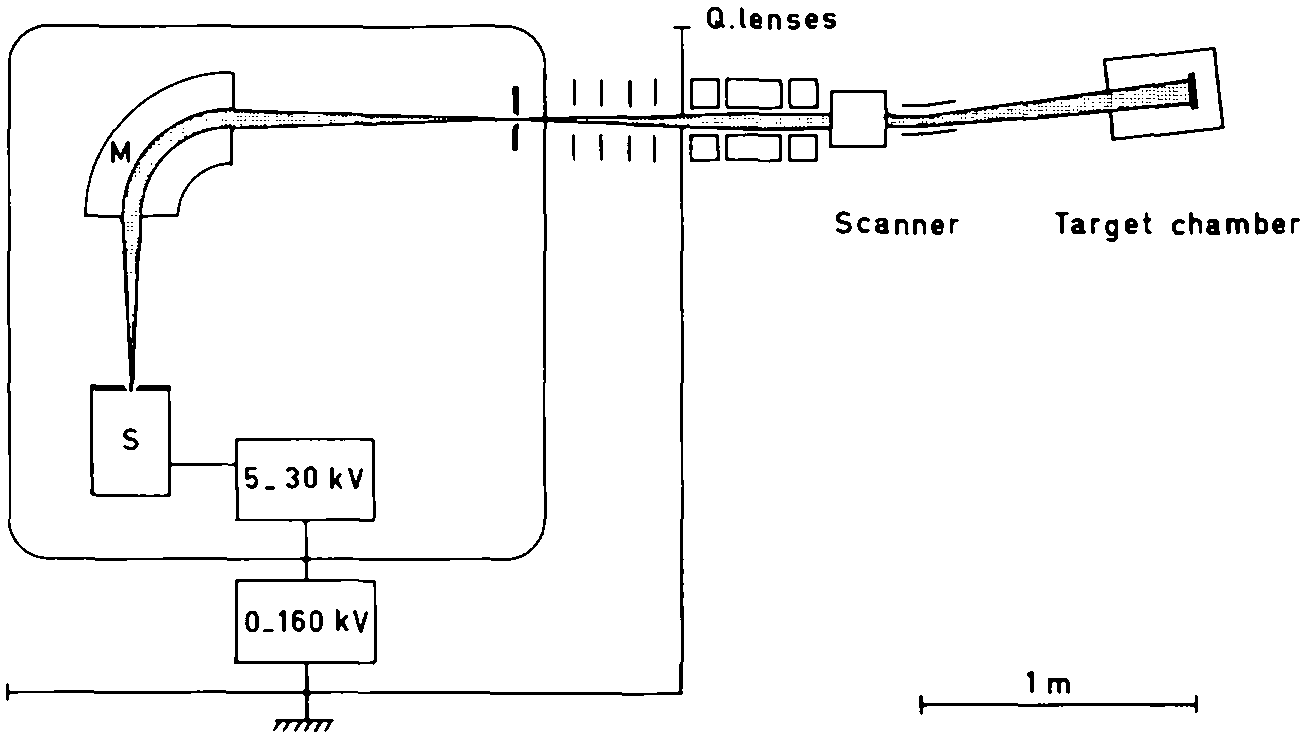
\includegraphics[width=\textwidth]{04_IPHI_Test/figures/fig000_IRMA01.png}
		\caption{}
		\label{}
	\end{subfigure}
	~
	\begin{subfigure}{0.5\textwidth}
		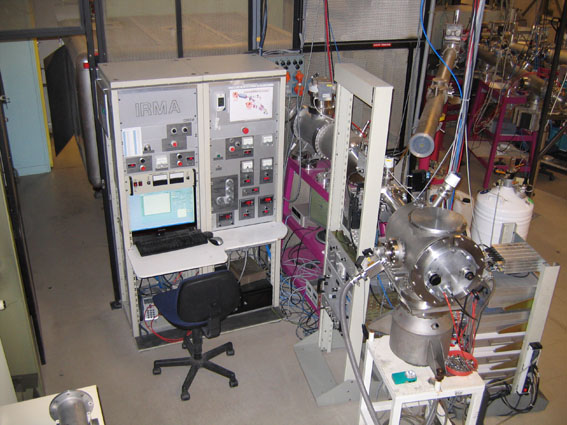
\includegraphics[width=\textwidth]{04_IPHI_Test/figures/fig000_IRMA02.jpg}
		\caption{}
		\label{}
	\end{subfigure}
	\caption[IRMA installation]{IRMA installation}
	\label{chap4:IRMA_facility}
\end{figure}


  \subsection{Test setup}

  The test bench consists of a mechanical support on which is mounted the detector system. The current range at IRMA is important (from hundred $\mathrm{pA}$ to $\mathrm{\mu A}$) compared to the expected ionization current per \acrshort{ess} pulse (few $\mathrm{fA}$). The average current has been reduced by the following solutions. The beam was scanned in both directions at $80 \,\mathrm{Hz}$ and $400\,\mathrm{Hz}$ on a perpendicular stopping plate. A hole was drilled at the center of the plate, reducing the current by a factor of $12723$. At the end, the number of incident particles was around hundred thousand (hundred $\mathrm{fA}$) per IRMA “pulse”. A simple Faraday cup measures the current after reduction. The entire setup is visible in Fig. \ref{chap4:IRMA_setup}.

  \begin{figure}[!ht]
	\begin{subfigure}[t]{0.5\textwidth}
		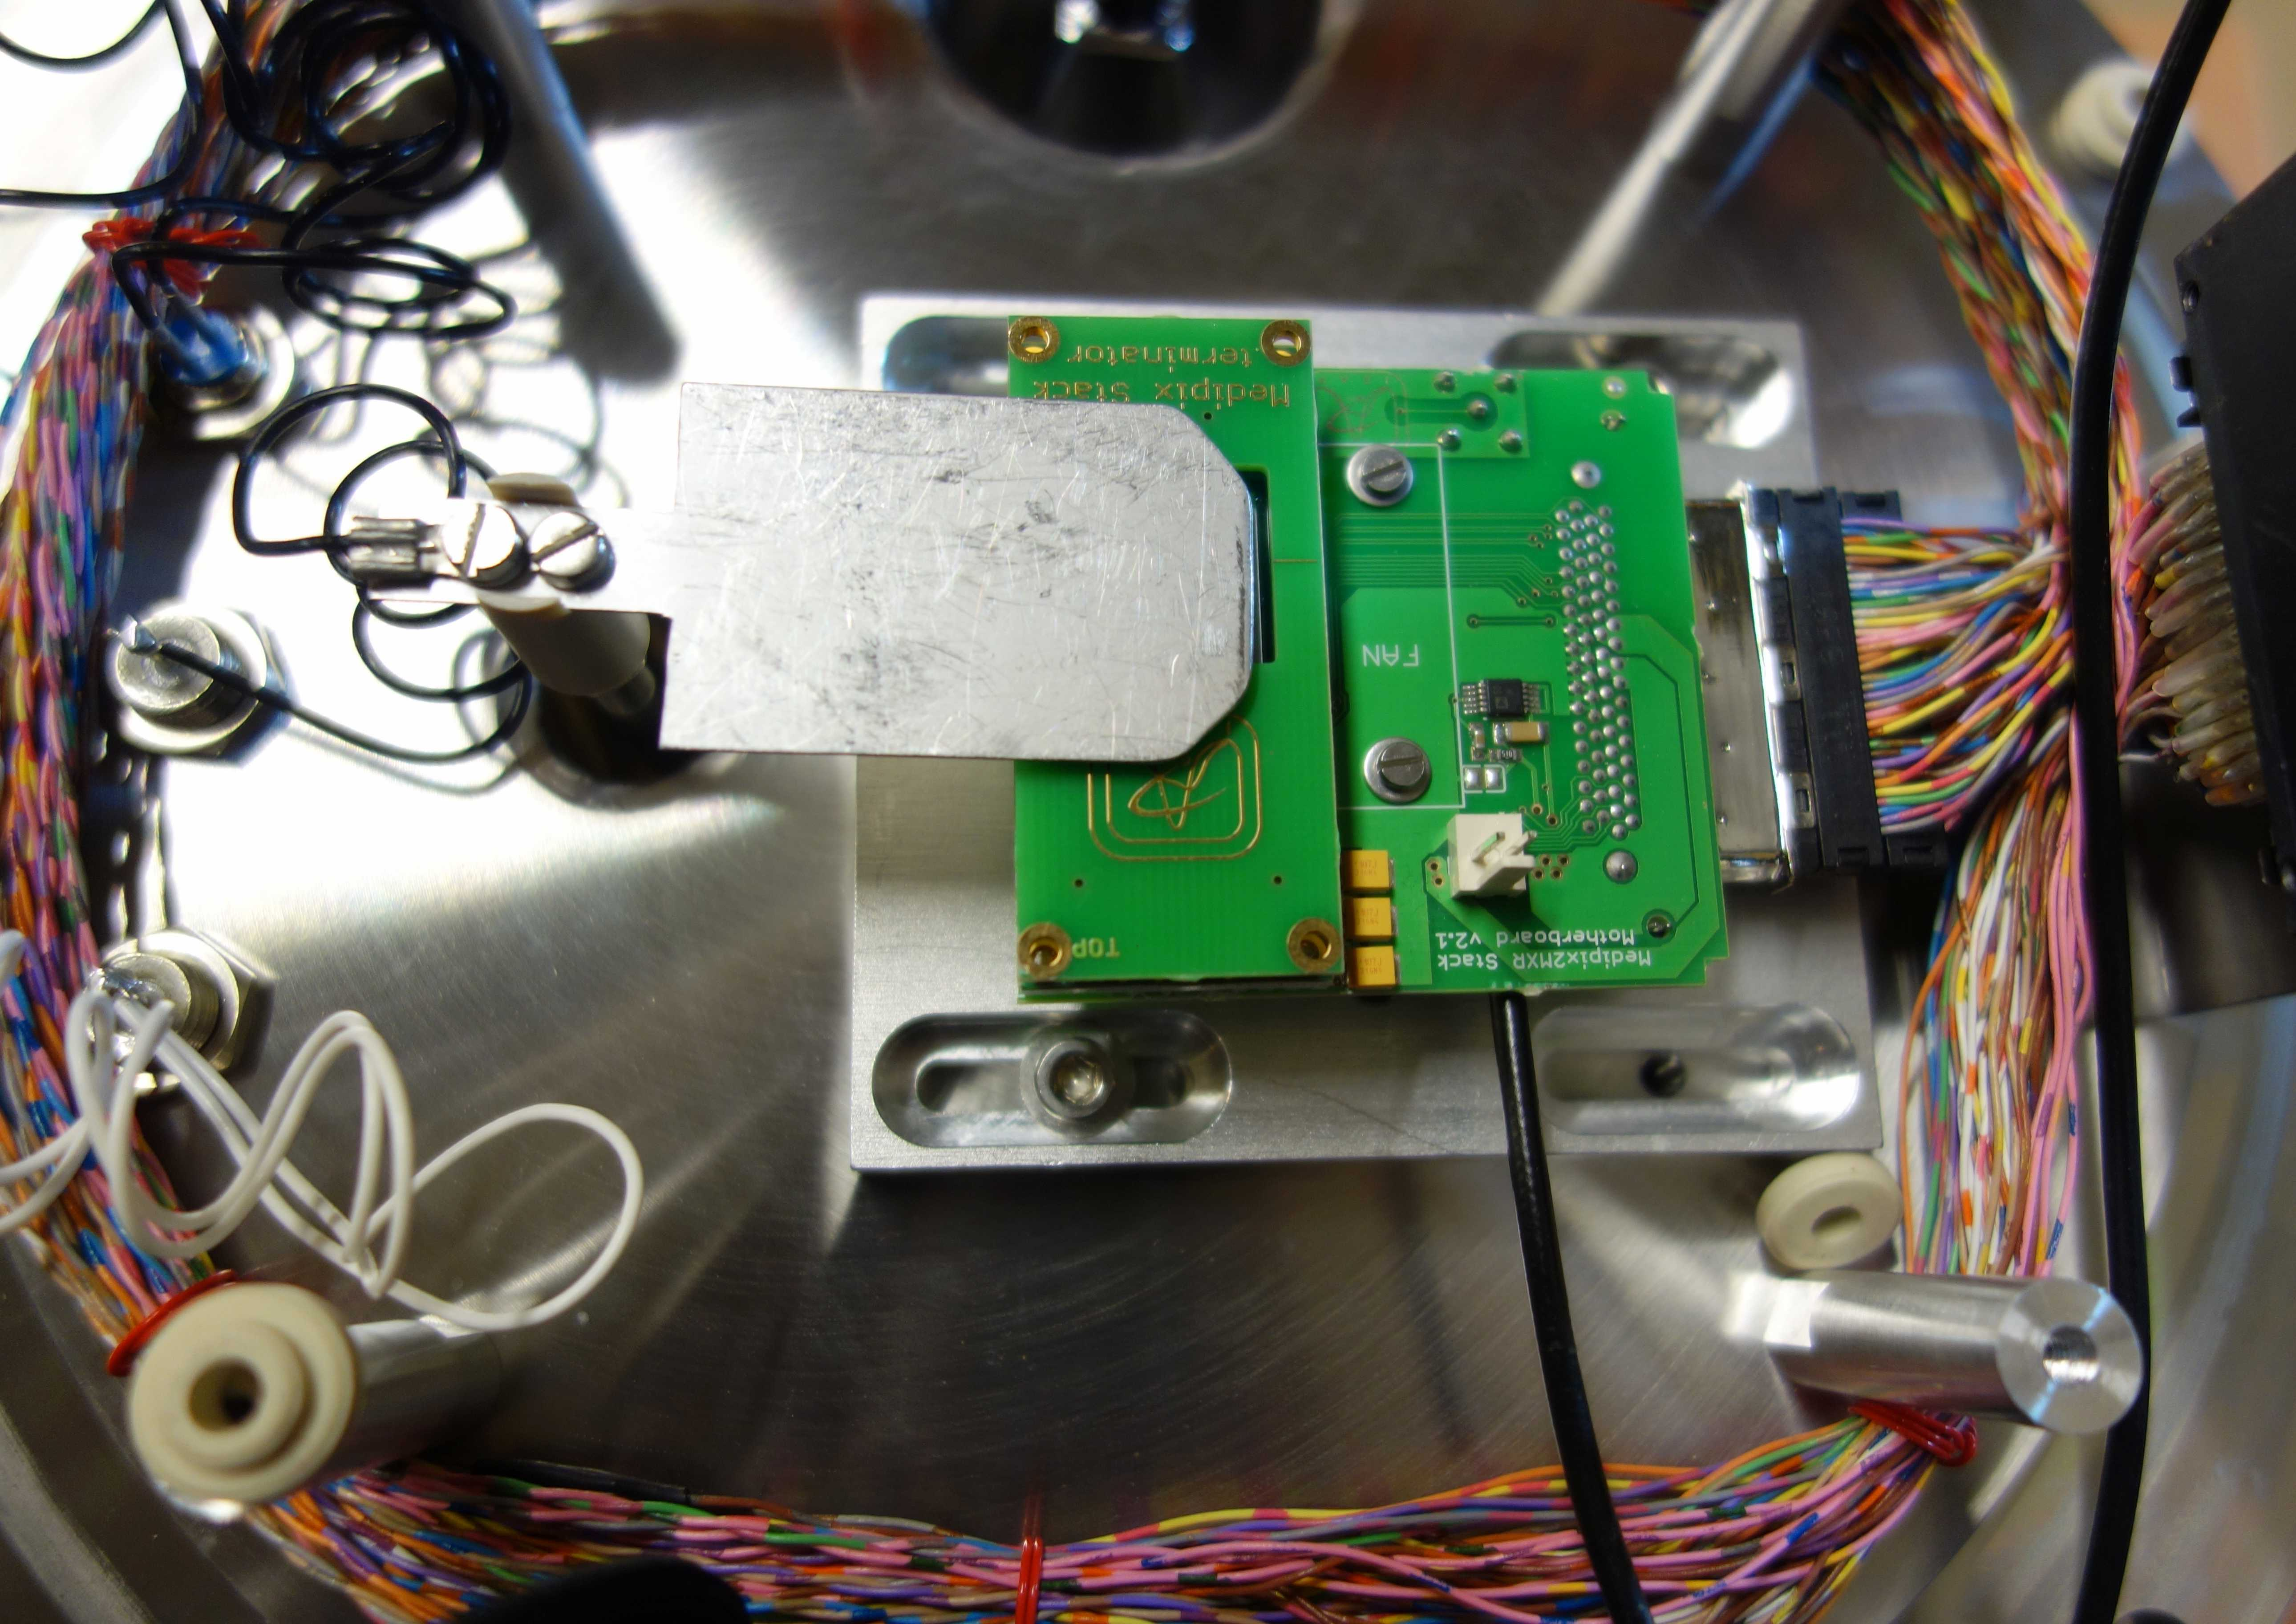
\includegraphics[width=\textwidth]{04_IPHI_Test/figures/fig000_IRMA_setup01}
		\caption{The TimePix chip is just behind the Faraday cup.}
		\label{}
	\end{subfigure}
	~
	\begin{subfigure}[t]{0.5\textwidth}
		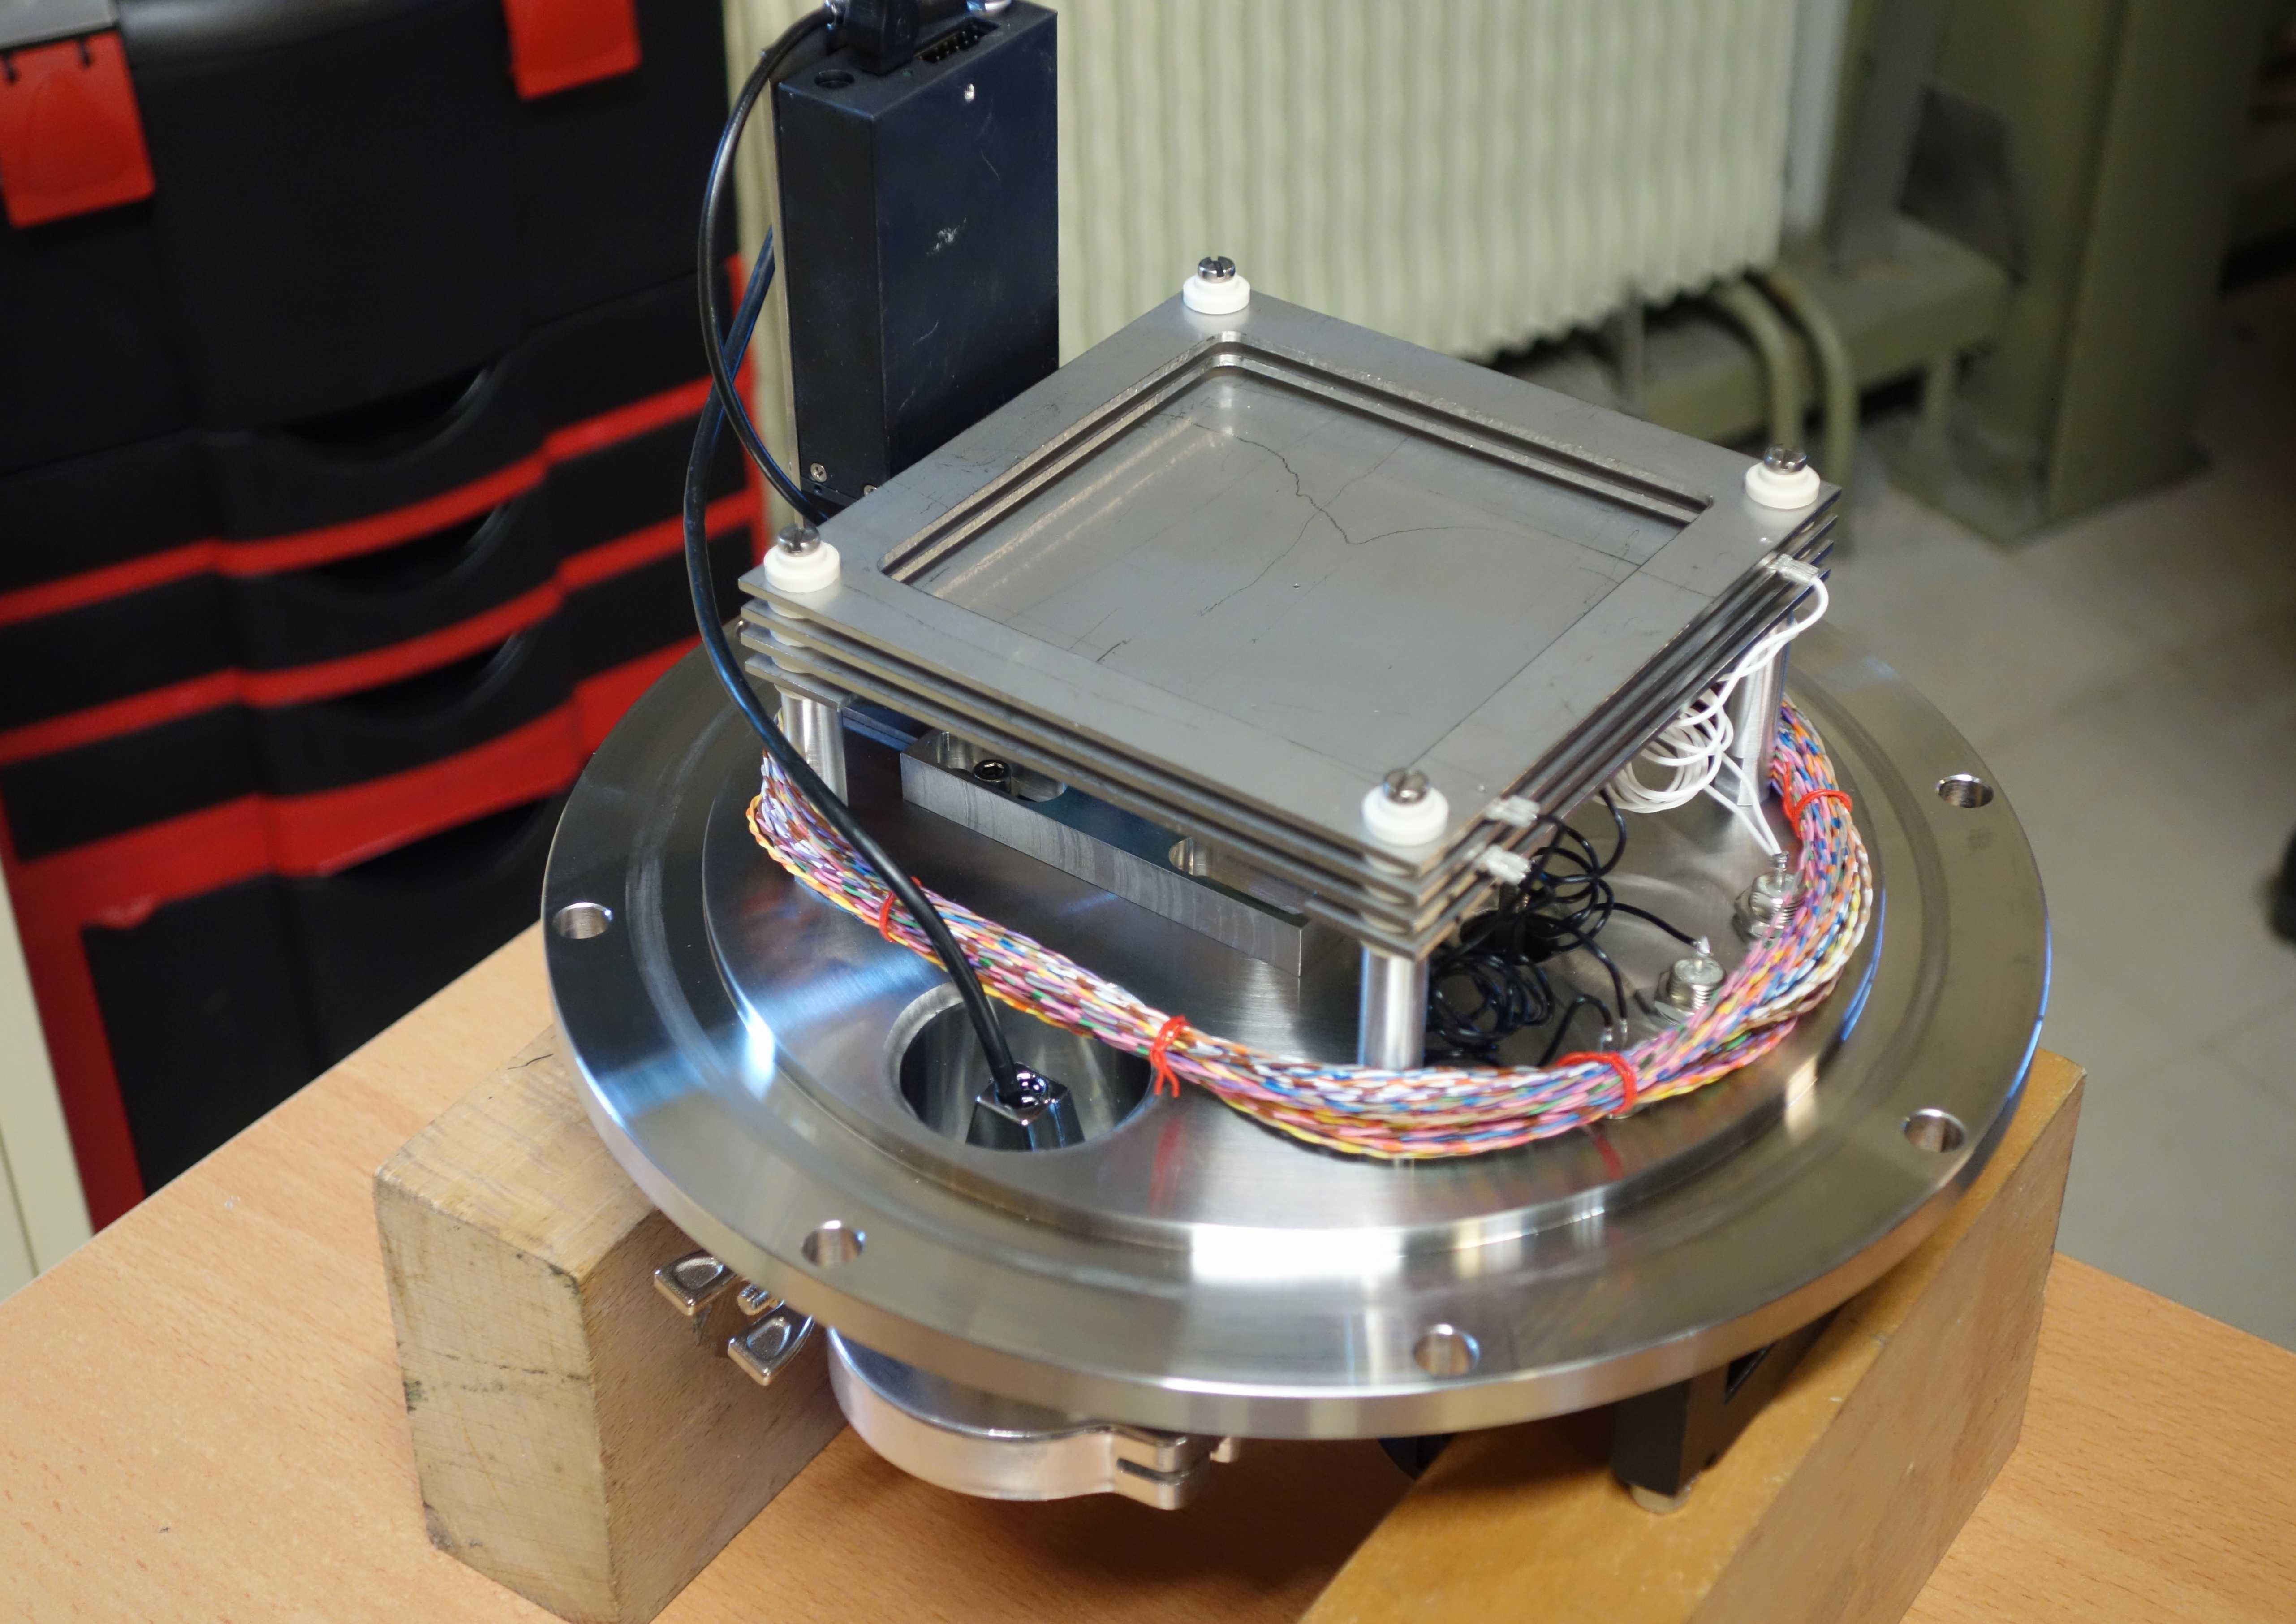
\includegraphics[width=\textwidth]{04_IPHI_Test/figures/fig000_IRMA_setup02}
		\caption{A plate with a drilled hole reduced the incoming current. The beam is scanned on the plate.}
		\label{}
	\end{subfigure}
	\caption[IRMA setup]{IRMA setup. A dedicated test bench has been developed for testing the TimePix chips.}
	\label{chap4:IRMA_setup}
\end{figure}


  The detector tested at IRMA is a silicon pixelated matrix ($256 \times 256$ with a pixel size $56\,\mathrm{\mu m}$) on top of a TimePix chip. The matrix is very specific since the metallization layer has been replaced by a heavily doped layer allowing the polarization of the detector. The TimePix measures either the Time over Threshold (ToT) or the Time of Arrival (ToA). ToT is the total time during which the signal generated by the incident particle is above a threshold set by the user. This value is therefore proportional to the energy deposited by the particles in the pixels. The ToA gives the time difference of an incident particle with respect to a reference time.

 The TimePix detector used was already equipped of a complete solution \cite{Kraus2011,advacam2019} integrating a readout electronics controllable by PC. The software allows to configure the TimePix and acquire images with the value of ToT or ToA for each pixel.

  \subsection{Results and limitations}

  The test performed at IRMA concerns the determination of the detection limit with the lightest possible ions i.e. $H_{2}^{+}$. The images at two energies and integrated signal for a full scan are shown in Fig. \ref{chap4:IRMA_Si}.
  
  \begin{figure}[!ht]
	\begin{subfigure}{0.25\textwidth}
		\includesvg[width=\textwidth]{04_IPHI_Test/figures/fig000_IRMA_15keV}
		\caption{ToT image at $15\,\mathrm{keV}$}
		\label{}
	\end{subfigure}
	~
	\begin{subfigure}{0.25\textwidth}
		\includesvg[width=\textwidth]{04_IPHI_Test/figures/fig000_IRMA_12keV}
		\caption{ToT image at $12\,\mathrm{keV}$}
		\label{}
  \end{subfigure}
  ~
  \begin{subfigure}{0.5\textwidth}
		\includesvg[width=\textwidth]{04_IPHI_Test/figures/fig000_IRMA_sweep}
		\caption{Total signal on the sensor with respect to the ion energies.}
		\label{}
  \end{subfigure}
	\caption[Main results from IRMA tests with $H_{2}^{+}$ ions]{Main results from IRMA tests with $H_{2}^{+}$ ions.}
	\label{chap4:IRMA_Si}
\end{figure}

  \begin{wrapfigure}{r}{0.4\textwidth}
  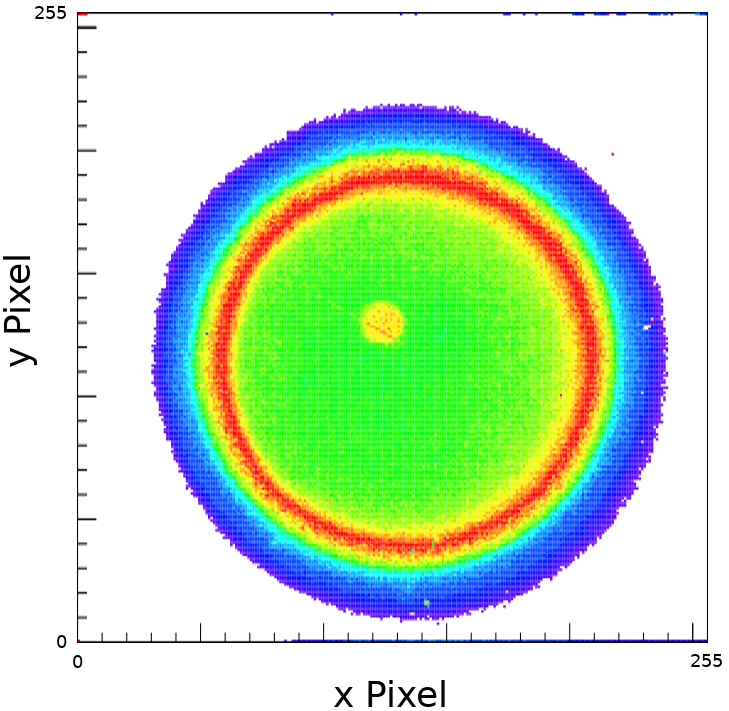
\includegraphics[width=0.4\textwidth]{04_IPHI_Test/figures/fig000_IRMA_damage2}
	\caption[The gain has changed after the irradiation]{The gain has changed after the irradiation.}
	\label{chap4:IRMA_damage}
\end{wrapfigure}

  The scan range is limited to few values because tuning the ion implanter to different energies was time consuming. For $15\,\mathrm{keV}$ ions the detection seems to work correctly, but the signal vanishes for ions with an energy of $12\,\mathrm{keV}$ or less. The limit of detection is therefore between these two values, and is very close to the energy that ions can reach in the \acrshort{ipm}s. The residual gas at \acrshort{ess} is mainly a compound of ions heavier than $H_{2}^{+}$. These heavy ions will not be detected by the readout, reducing the already low signal of the \acrshort{ipm}. One can see that the point at $20\,\mathrm{keV}$ is unlikely. The measurement for this point was performed at the end of the day after few hours of irradiations at low energy. Ideally we should have taken more measurements at different energies.

  Few days after the test, the integrity of the sensor has been tested by illuminating it with an UV-VIS LED (peak emission at 365 nm). 
Fig. \ref{chap4:IRMA_damage} shows a small zone of the pixel matrix with different gain, corresponding to the IRMA beam position irradiation.
Clearly the sensor was damaged, but unfortunately we can not give an accurate estimation of the deposited dose. Note that the gain has increased in the irradiated region whereas we expect a reduction as we observed at IRMA.
  % A zone in the matrix and it is visible in Fig. \ref{chap4:IRMA_damage}.
  % This zone is exactly in the same place as the one bombarded by the ions. The sensor has been probably deteriorated by the high current of IRMA. Unfortunately it is not possible to accurately estimate the number of ions that have been sent to the sensor and the nature of the damage is unknown. 

 At last we decided to discard the possibility of using silicon detectors because of the signal weakness, not compliant with \acrshort{ipm}s working in the mandatory ion mode, and for the damages induced by ions as previously seen. The development cost of a silicon solution is not worth considering the possible risks of non-detection.
  In our quest for feasibility demonstration, we faced several issues:
  \begin{itemize}
    \item Triggered acquisitions were not possible, imposing to take long integration time to avoid missing the beam interaction with the silicon detector.
    \item Consequently, despite calculations, the beam sweeping on the detector varied from time to time explaining partly our impossibility to evaluate the dose.
    \item The data campaign was concentrated on a single day. We discovered the facility and its constraints at the same time as dealing with our measurements.
  \end{itemize}

Still, we hope to have the opportunity to retest the silicon detector at IRMA, or at another ion implanter facility, to fully determine the ion detection limit and investigate more on ion damaging. 
Nowadays, TimePix3 has completely replaced its ancestor. This new integrated circuit provides the ability to measure at a same time the ToT and ToA, with a higher timing resolution and an efficient data protocol. Also, the readout electronics has been improved allowing advanced triggering option of the chip.

  % We decided to not go further with silicon detectors for all the previous reasons. The cost of development of a silicon solution is not worth considering the possible risks of non detection. We would like to remain that the experiment has been done to quickly check the feasibility and it suffers from several limitations. Firstly the detector was not triggered, during short acquisitions pulse only very few data were taken in coincidence with the beam, therefore long acquisitions have been favored reducing the uncertainty only on the first and last pulse. The second uncertainty comes from the beam scanning. We noticed that, sometimes, the beam could pass through the hole more than once for a same scanning cycle. This means that the number of charge is collected by the TimePix is more than expected for an acquisition.


  \section{IPM design overview}
  \subsection{IPM}
  %\begin{figure}[!ht]  
  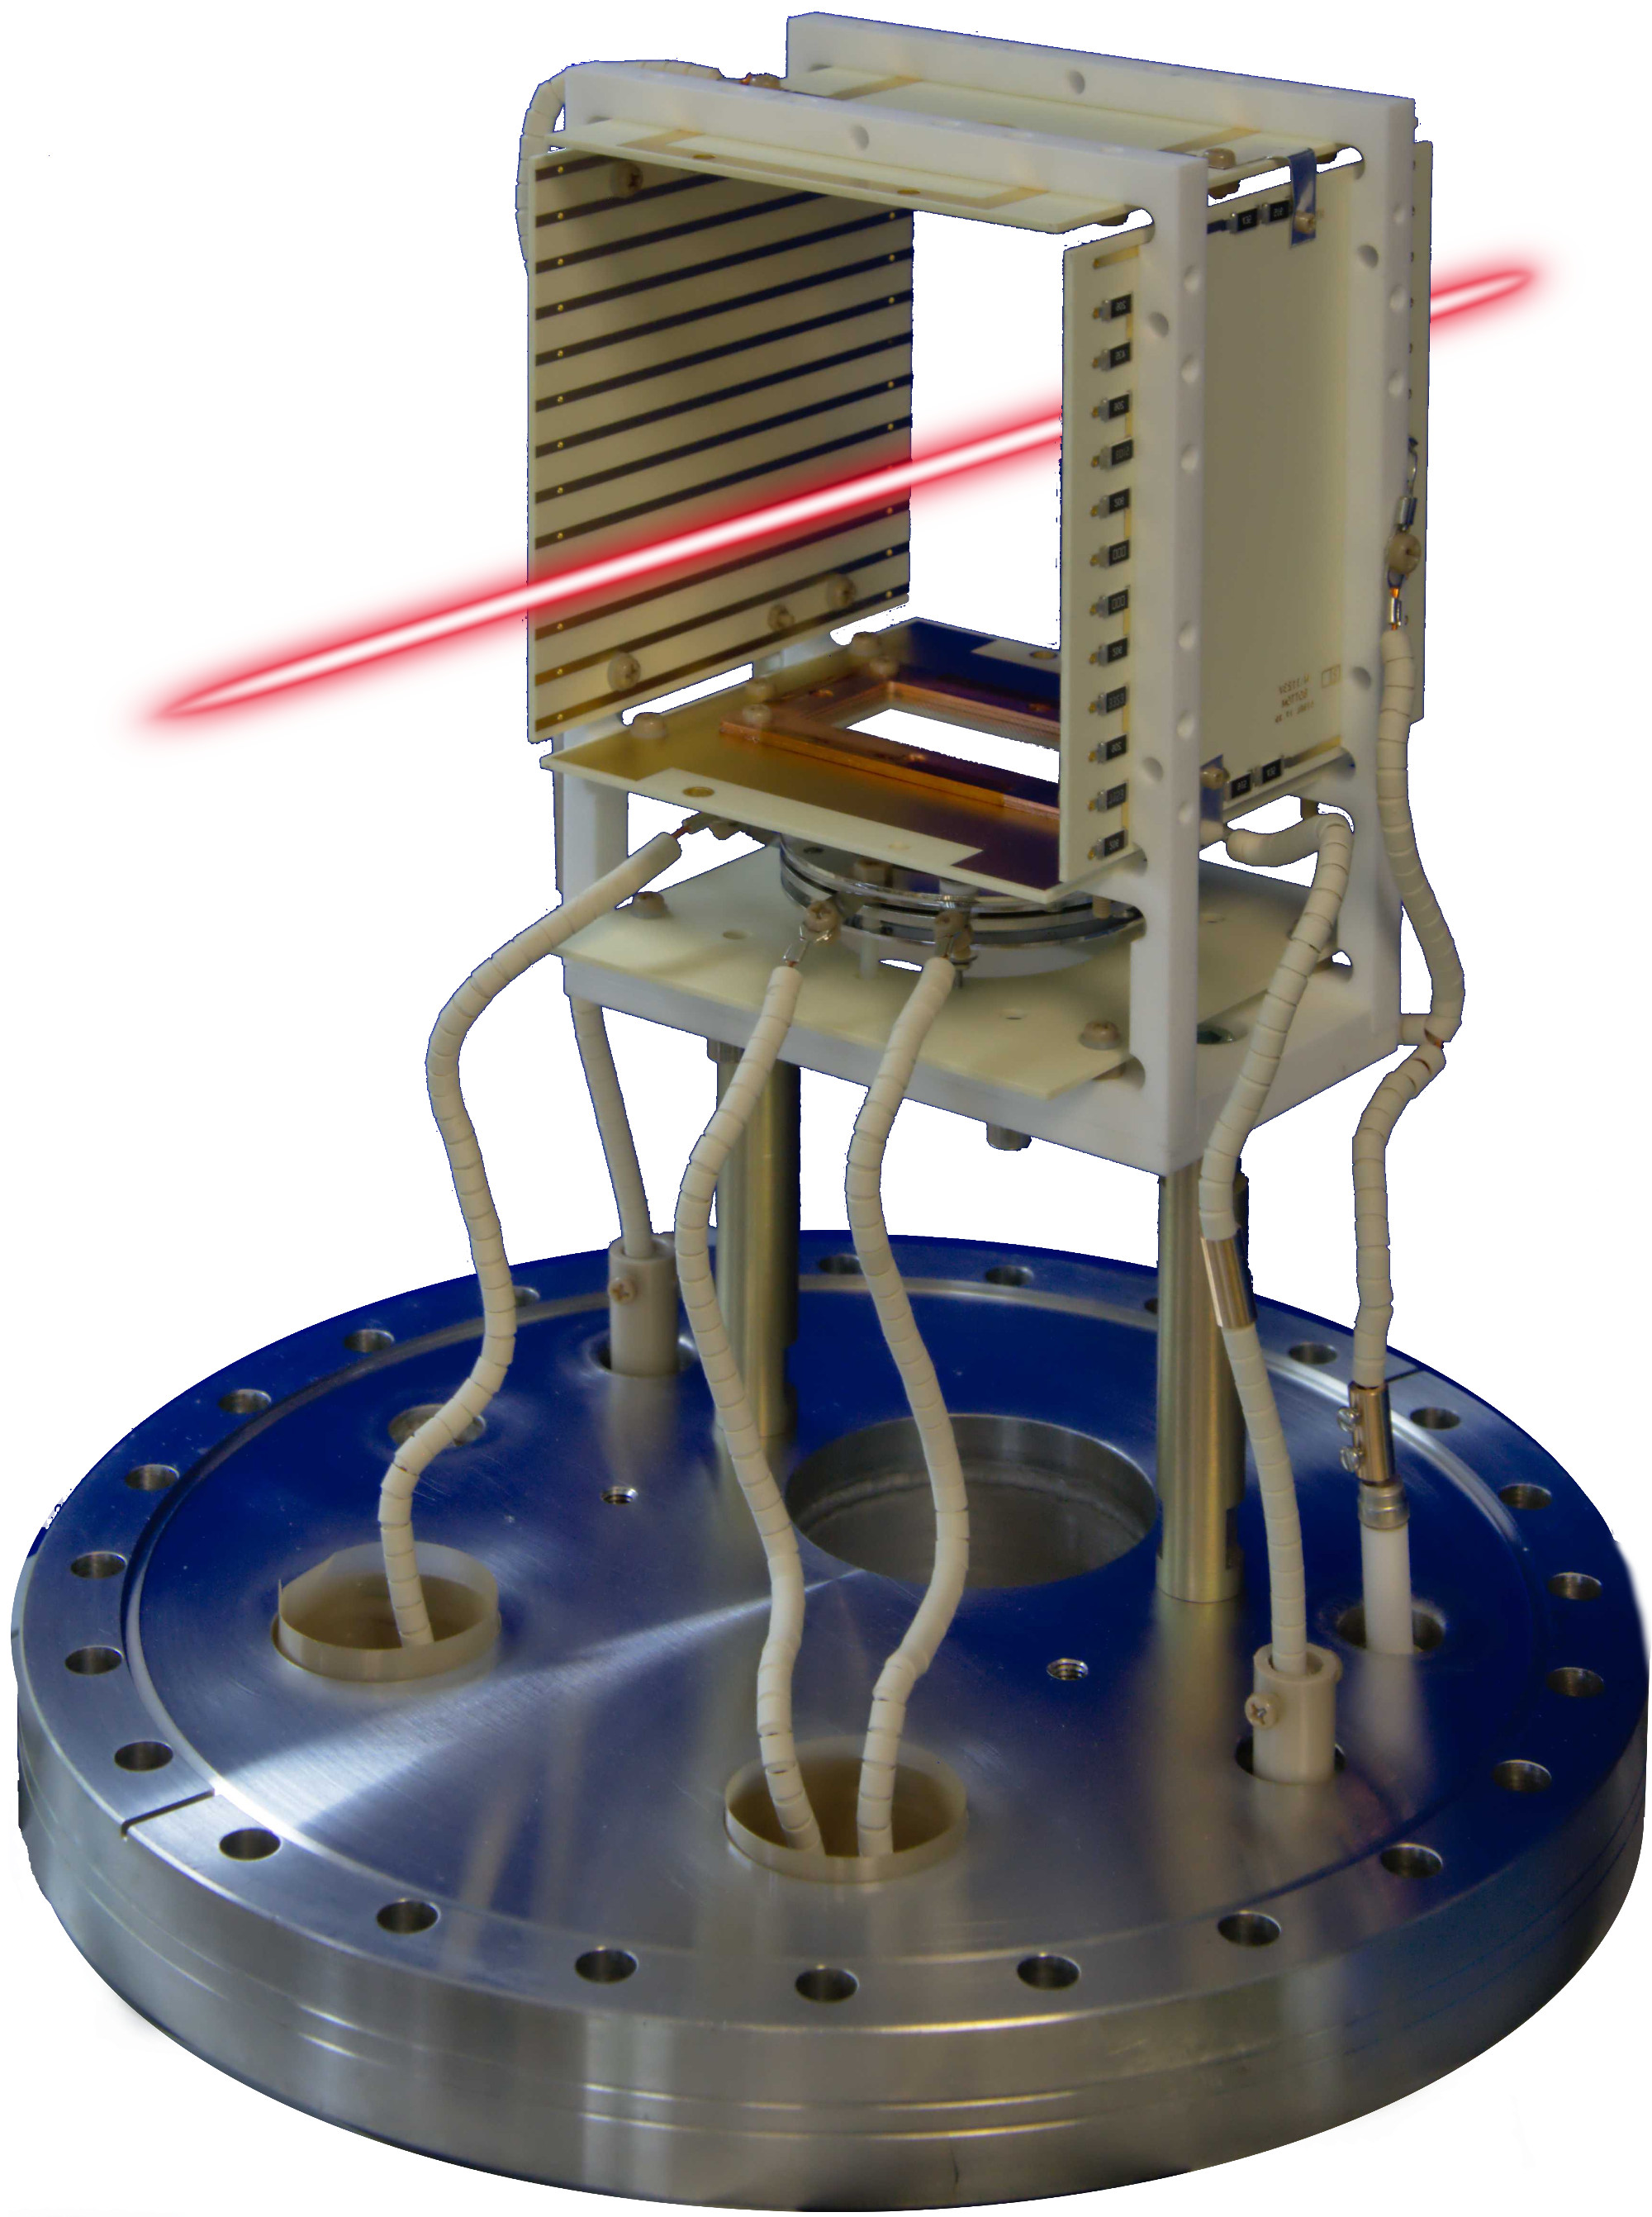
\includegraphics[width=0.8\textwidth]{04_IPHI_Test/figures/fig000_IPM_photo2}
  \caption[One of the IPM prototypes]{One of the IPM prototypes. The MCP is visible below the cage.} %The field corrector plate are due to the presence of resistor.}
  \label{chap4:IPM_photo2}
\end{figure}

  The \acrshort{ipm} consists of five \acrshort{pcb} plates: two for the electrodes, two for the field correctors and one for supporting the readout. The two electrode plates face each other, as well as the correction plates. The electrode closest to the readout is grooved in its center with a conductive grid fixed on it, for insuring the electric field uniformity (see explanations on the previous chapter). The top electrode has a $5.5\,\mathrm{mm}$ radius circular hole in its center to allow illumination from a calibration source. The field correctors were engraved directly on the inner \acrshort{pcb} face and resistors are welded on the outer side. SMD resistor type $2512$ ($1\,\mathrm{\%}$ precision, $3000\,\mathrm{V}$ max) are used.

  All \acrshort{pcb} boards are firmly encapsulated in two frames made of insulating material. Two materials have been used: PEEK and MACOR. MACOR is a machinable ceramic that provides very high electrical insulation (more than $50\,\mathrm{kV/mm}$ DC), good thermal conduction and withstands high temperatures ($800\,\mathrm{\textdegree{}C}$). It is also compatible with vacuum despite its porous appearance. Even if it has very interesting mechanical properties, it must be handled with care \footnote{The author personally attest this fact after he screwed too tightly on a frame MACOR.}. PEEK (Polyether Ether Ketone) is a plastic polymer used in aggressive chemical environments. It is both an electrical (around $16\,\mathrm{kV/mm}$) and a thermal insulator. It does not tolerate temperatures above $250\,\mathrm{\textdegree{}C}$. PEEK can be used under vacuum, but its performance is much lower than MACOR. On the other hand, it is cheaper and easier to handle.

  The two frames are screwed to a MACOR support fixed on the flange via two stainless steel rods. The ceramic support ensures a perfect insulation of the \acrshort{ipm} with the vacuum chamber. The \acrshort{ipm}s has been designed so that the cage is completely independent of the readout used. For \acrshort{ipm}s using strips, it is also possible to rotate the \acrshort{ipm} by $90\,\textdegree{}$ to change the direction of the measurement. The connections to the different high voltages are wired with bare copper protected by ceramic beads. Vacuum feedthroughs are COTS components that can support voltages up to $30\,\mathrm{kV}$.

  An \acrshort{ipm} prototype fully mounted on its flange is pictured in Fig. \ref{chap4:IPM_photo2}.

  \begin{figure}[!ht]  
  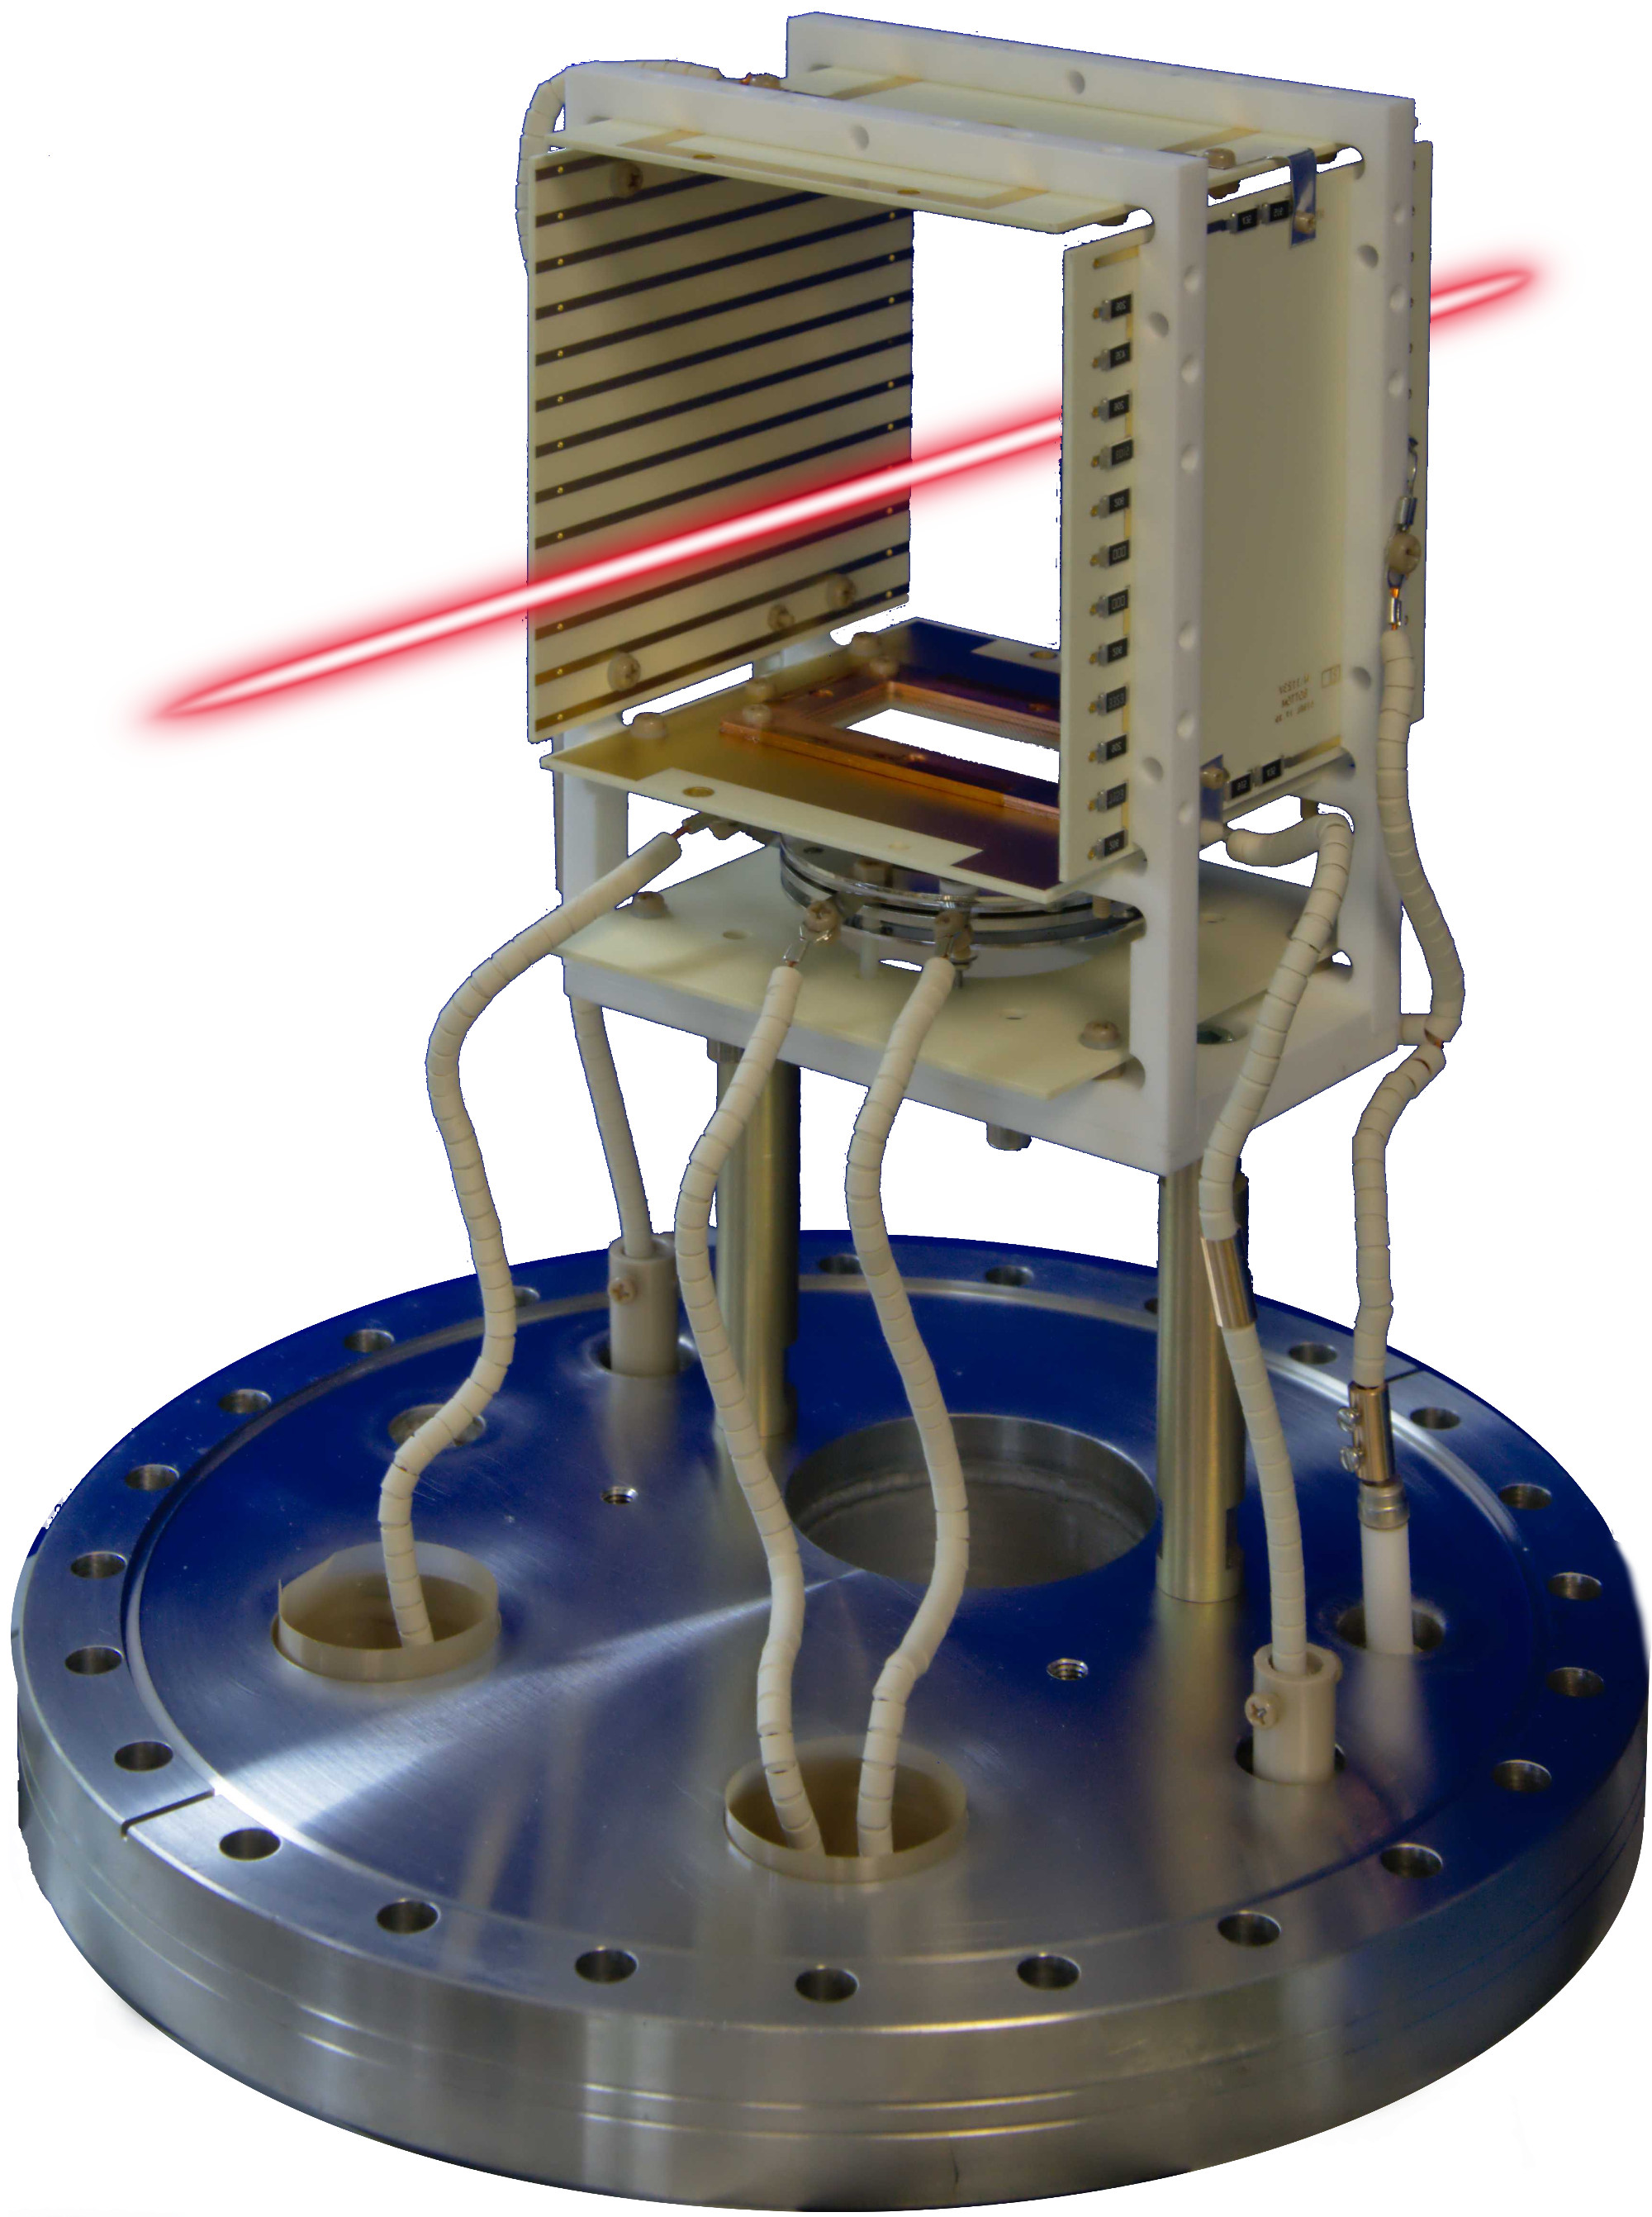
\includegraphics[width=0.8\textwidth]{04_IPHI_Test/figures/fig000_IPM_photo2}
  \caption[One of the IPM prototypes]{One of the IPM prototypes. The MCP is visible below the cage.} %The field corrector plate are due to the presence of resistor.}
  \label{chap4:IPM_photo2}
\end{figure}


  \subsection{MCP}
  A total of four \acrshort{mcp}s has been bought from two different suppliers, Hamamatsu and Photonis: a simple single stage \acrshort{mcp} and a single stage \acrshort{mcp} coupled with a phosphorus screen. The simple \acrshort{mcp}s will be used with the strips \acrshort{ipm}s if the signal becomes too low.

  The \acrshort{mcp} and phosphorus assemblies are key components of the optical \acrshort{ipm}s and two different phosphorus screens were considered:
  \begin{itemize}
    \item P43 is a very luminescent material but has a strong remanence.
    \item P46 has a fast decay time but lower yield.
  \end{itemize}
  Since intra-pulse acquisition is not a requirement for \acrshort{ess} both screens may be considered.

  The characteristics of each \acrshort{mcp} (and phosphorus screen) are given in the Table \ref{chap4:MCP_Phosphor}.
  \begin{table}[ht]
  \centering
  \caption[The main characteristics of MCPs used during the beam tests]{The main characteristics of MCPs used during the beam tests. MCPs from Hamamatsu has the same characteristics except that one has a phosphorus screen as readout.}
  \label{chap4:MCP_Phosphor}
  \begin{tabular}{llll}
    \toprule
                     & Hamamatsu         & Photonis 1                  & Photonis 2                  \\
    \midrule
    Active radius    & $40\,\mathrm{mm}$           & $40\,\mathrm{mm}$           & $40\,\mathrm{mm}$           \\
    Channel diameter & $12\,\mathrm{\mu m}$        & $10\,\mathrm{\mu m}$        & $25\,\mathrm{\mu m}$        \\
    Channel pitch    & $15\,\mathrm{\mu m}$        & $12\,\mathrm{\mu m}$        & $32\,\mathrm{\mu m}$        \\
    OAR              & $60\,\mathrm{\%}$           & $55\,\mathrm{\%}$           & $45\,\mathrm{\%}$           \\
    Bias angles      & $8\,\mathrm{\textdegree{}}$ & $8\,\mathrm{\textdegree{}}$ & $8\,\mathrm{\textdegree{}}$ \\
    \midrule
    Screen type      & $P43$                  & $P46$                       & -                           \\
                     & $Gd_{2}O_{2}S:Tb$           & $Y_{3}Al_{5}O_{12}:Ce$      &                             \\
    Gain relative    & $1$                      & $0.3$                       & -                           \\
    Wavelength       & $545\,\mathrm{nm}$      & $530\,\mathrm{nm}$          & -                           \\
    Decay time range & $\mathrm{ms}$           & $\mathrm{\mu s}$            & -                           \\
    \bottomrule
  \end{tabular}
\end{table}

  \subsection{Camera}
  A vision system is necessary for recording light from the phosphorus screen.
  A camera with a lens should be sufficient in our case.

  % Sensor
  The sensor is the core component of a camera, so it is better to choose it first, on the basis of the requirements.
  For our application high resolution is not mandatory, so pixels could be relatively large in order to increase light collection and dynamic range.
  Sony IMX249 fits well with these prerequisites. It is a consumer \acrshort{cmos} sensor with big pixels and low noise.
  Its EMVA characteristics are summarized in the Table \ref{tab:IMX249} \cite{emva2010}.
  \begin{table}[!h]
  \centering
  \caption{Main features of the Sony IMX249 sensor}
  \label{tab:IMX249}
  \begin{tabular}{ll}
    \toprule
    Resolution           & 1936 (H) * 1216 (V)  \\
    Pixel size           & 5.86 $\mu m$         \\
    Sensor diagonal size & 13.4 mm (Type 1/1.2) \\
    Well capacity        & 32000 e-             \\
    Dynamic Range        & 70 dB                \\
    QE at 525 nm         & 70 \%                \\
    Electrons noise      & 6.8 $e^{-}$          \\
    ADC                  & 8, 10 or 12 bits     \\
    Max framerate        & 30 fps               \\
    \bottomrule
  \end{tabular}
\end{table}

  % Camera
  AlliedVision, Basler and FLIR propose several cameras based on the IMX249 sensor with different interfaces, features, form factors, prices and availability.
  We restricted our choice to GigE cameras since they allow long cable length and Power over Ethernet (PoE) which are quite useful features for an accelerator experiment.
  At the end, we chose the FLIR Blackfly-PGE-23S6M-C \cite{blackfly2019}.

  % Lens
  The last step is the choice of a correct lens for the camera.
  Unfortunately lens suppliers do not provide full characteristics of their lenses, hence only the thin lens approximation has been considered in our calculations. The distance from the back of the phosphorus screen to the external air-side of the viewport is $247\,\mathrm{mm}$. The active area radius of our \acrshort{mcp}s is around $25\,\mathrm{mm}$, while the sensor side measures $11.34\,\mathrm{mm}$. The required magnification therefore amounts to $0.2268$ at least.
  Table \ref{tab:lens_magnification} shows magnification factors for several focal lengths. So, a focal length of $50\,\mathrm{mm}$ fits very well with our configuration.
  \begin{table}[!h]
  \centering
  \caption[Magnification for several common focal lengths]{Magnification for several common focal lengths, at a working distance of $247\,\mathrm{mm}$.}
  \label{tab:lens_magnification}
  \begin{tabularx}{1\textwidth}{lllllllll}
    \toprule
    Focal length ($\mathrm{mm}$) & $5$    & $15$    & $28$    & $35$    & $50$    & $75$    & $100$  & $150$   \\
    Magnification     & $0.02$ & $0.069$ & $0.127$ & $0.165$ & $0.255$ & $0.436$ & $0.68$ & $1.546$ \\
    \bottomrule
  \end{tabularx}
\end{table}

  Lenses with $50\,\mathrm{mm}$ focal length are rather standard and commercially available at moderate cost. In addition these lenses have a large numerical aperture (or small F-number) so they provide a large photon capture efficiency.

  \subsection{Strips}

  The strips were manufactured in the same way as the other \acrshort{pcb}s presented above. Two strip configurations have been foreseen. The first one is the linear strips: the strips have the same width of $800\,\mathrm{\mu m}$ and an identical spacing of $920\,\mathrm{\mu m}$. A total of 32 strips were etched on the \acrshort{pcb}, representing an active area of about $3\,\mathrm{cm}$. The second version is called Gaussian because the strips on the borders are wider than the ones in the center. The idea is that the strips on edges detect only few particles, so it is not necessary to have very thin strips since they will probably be in the noise. Therefore, the number of strips is reduced to $18$ with variable width from $0.8\,\mathrm{mm}$ to $9\,\mathrm{mm}$, leading to a total active area of $5\,\mathrm{cm}$. The table gives the values for the first $9$ gaussian strips, the $9$ remaining strips are the mirror of the first ones.

  \begin{table}[!ht]
  \centering
  \caption[Positions and sizes of the first half of gaussian strips]{Positions and sizes of the first half of gaussian strips.}
  \label{chap4:GaussianStrips}
  \begin{tabularx}{\linewidth}{lXXXXXXXXX}
    \toprule
    Strip    & 1     & 2    & 3    & 4    & 5    & 6    & 7    & 8    & 9    \\
    \midrule
    Size ($\mathrm{mm}$)    & 9     & 5    & 3    & 2    & 1.5  & 1    & 0.9  & 0.8  & 0.8  \\
    Position ($\mathrm{mm}$) & 20.52 & 13.4 & 8.28 & 6.66 & 4.79 & 3.42 & 2.35 & 1.38 & 0.46 \\
    \bottomrule
  \end{tabularx}
\end{table}
%   \centering
%   \setlength\tabcolsep{1.5pt}
%   \scalebox{0.8}{
%     \begin{tabular}{l| c |c | c } \hline \hline
%       STRIP NUMBER  \hspace*{1.5cm} & \hspace*{0.75cm} x\_min \hspace*{0.75cm} & \hspace*{0.75cm} x\_max \hspace*{0.75cm} & \hspace*{0.75cm} width \hspace*{0.75cm} \\
%       \hline \hline
%       1                             & -25.02                                   & -16.02                                   & 9                                       \\
%       2                             & -15.9                                    & -10.9                                    & 5                                       \\
%       3                             & -10.78                                   & -7.78                                    & 3                                       \\
%       4                             & -7.66                                    & -5.66                                    & 2                                       \\
%       5                             & -5.54                                    & -4.04                                    & 1.5                                     \\
%       6                             & -3.92                                    & -2.92                                    & 1                                       \\
%       7                             & -2.80                                    & -1.90                                    & 0.9                                     \\
%       8                             & -1.78                                    & -0.98                                    & 0.8                                     \\
%       9                             & -0.86                                    & -0.06                                    & 0.8                                     \\
%       10                            & 0.06                                     & 0.86                                     & 0.8                                     \\
%       11                            & 0.98                                     & 1.78                                     & 0.8                                     \\
%       12                            & 1.9                                      & 2.8                                      & 0.9                                     \\
%       13                            & 2.92                                     & 3.92                                     & 1                                       \\
%       14                            & 4.04                                     & 5.54                                     & 1.5                                     \\
%       15                            & 5.66                                     & 7.66                                     & 2                                       \\
%       16                            & 7.78                                     & 10.78                                    & 3                                       \\
%       17                            & 10.9                                     & 15.9                                     & 5                                       \\
%       18                            & 16.02                                    & 25.02                                    & 9                                       \\
%       \hline \hline
%     \end{tabular}}
%   \caption{Gaussian detector geometry.}
%   \label{tab:det2}
% \end{table}

  \subsection{CARAMEL board and FASTER system}

  The strips are read by the \acrshort{caramel} card \cite{caramel2013} from the \acrshort{faster} system. \acrshort{faster} is a versatile acquisition platform developed by LPC at Caen \cite{faster2013}. \acrshort{caramel} is an electrometer VITA-57 card based on two DDC316 chips from Texas Instrument \cite{ddc316}. Each chip integrates 16 acquisition channels connected to a dual integrator circuit allowing continuous measurement, as shown in Fig. \ref{chap4:DDC316}. The DDC316 chip covers integration times from $10\,\mathrm{\mu s}$ to $1\,\mathrm{ms}$ and three measurement ranges are available: $3\,\mathrm{pC}$, $6\,\mathrm{pC}$, $12\,\mathrm{pC}$. The DDC316 can read only positive charges, so an homemade current injector has been developed to add an offset allowing the measurement of negative charges.
  \begin{figure}[!ht]
	\begin{center}
		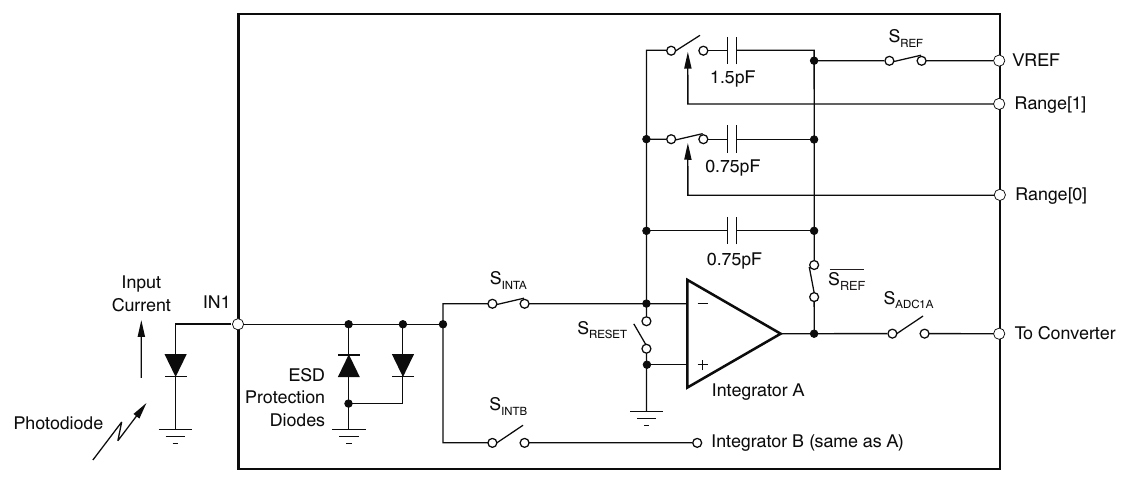
\includegraphics[width=\textwidth]{04_IPHI_Test/figures/fig000_DDC316}
	\end{center}
	\caption[]{}
	\label{chap4:DDC316}
\end{figure}


  Two \acrshort{caramel} boards can be plugged in a motherboard compatible with microTCA crates. All modules in a crate are controlled by a software that configures the entire system, runs acquisitions and visualizes \cite{rhb2012} the data online. The data can be saved in a binary format and a library allows to read them afterwards.

  \subsection{High voltage power supplies}
  An \acrshort{ipm} requires high voltages to create the extraction field and to supply the \acrshort{mcp} when it is used as readout. All power supplies come from iseg-HV \cite{iseg2019} and cover range from $0\,\mathrm{kV}$ to $30\,\mathrm{kV}$ with negative or positive polarities.

  \acrshort{mcp}s allow complete floating configuration. This means that the readout can work at very high potential. We refer to this configuration as symmetric since the \acrshort{mcp} is at the opposite value of the extracting electrode, as explained in the previous chapter. In this case, the electric field is more uniform if no corrections are applied. However, it increases the number of high voltage power supplies and the design complexity (Fig. \ref{chap4:setup_hv_sym}).
  Of course \acrshort{mcp}s work also correctly at ground potential (Fig. \ref{chap4:setup_hv_asym}) and we refer to this set-up as asymmetric. The strips \acrshort{ipm}s support only the asymmetric configuration and do not require more than one high voltage. During the two test campaigns we were able to work in both configurations.

  \begin{figure}[!ht]
  \begin{subfigure}[t]{0.5\textwidth}
    \centering
    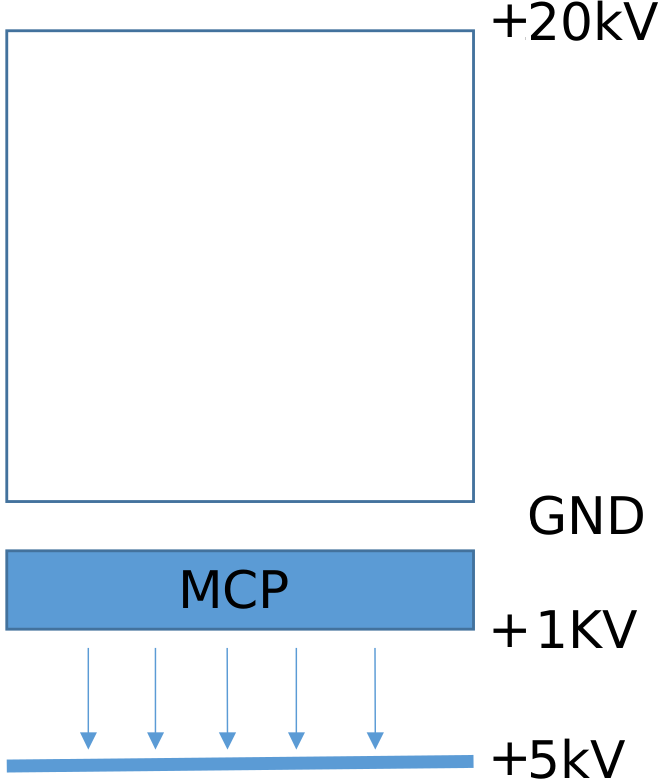
\includegraphics[width=0.7\textwidth]{04_IPHI_Test/figures/fig000_setup_hv_asym2}
    \caption{Asymmetric configuration.
    Readout is grounded while extracting electrode is at a certain potential.}
    \label{chap4:setup_hv_asym}
  \end{subfigure}
  ~
  \begin{subfigure}[t]{0.5\textwidth}
    \centering
    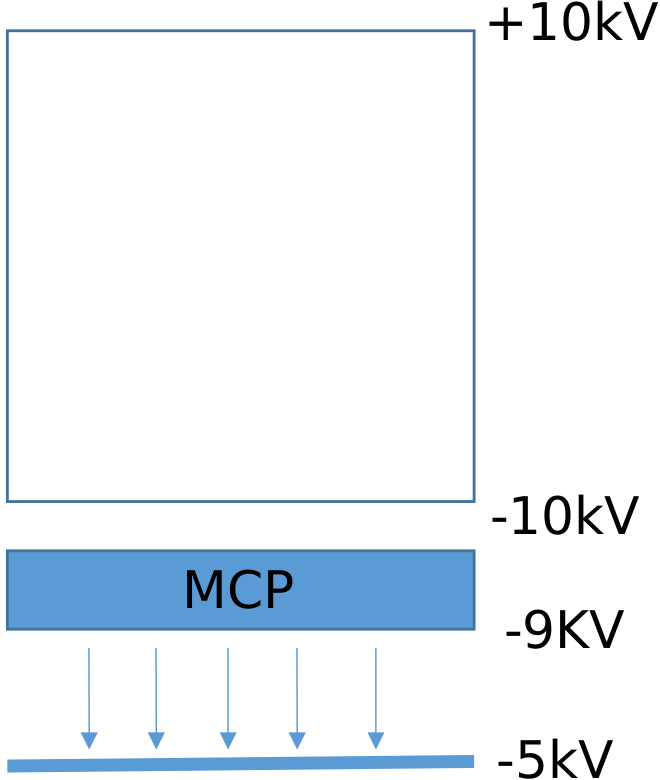
\includegraphics[width=0.7\textwidth]{04_IPHI_Test/figures/fig000_setup_hv_sym}
    \caption{Symmetric configuration. Readout and extracting electrode are at opposite potential.}
    \label{chap4:setup_hv_sym}
  \end{subfigure}
  \caption[Asymmetric or symmetric configuration]{Asymmetric or symmetric configuration, MCPs allow both.}
  \label{chap4:setup_hv}
\end{figure}


  \subsection{Control System}
  The whole \acrshort{ess} Control System (\acrshort{cs}) will rely on the Experimental Physics and Industrial Control System (\acrshort{epics}) toolkit. The \acrshort{ess} CS team has specified its own EPICS standards to ensure the sustainability of the control system over the years. We will also test our \acrshort{ipm}s at an accelerator whose control system is EPICS compatible. Therefore, EPICS has some importance to our project and we tried to use it as much as possible for our prototypes. In this section we will briefly describe EPICS and how we have integrated our test bench under such environment.

  EPICS provides a set of tools and protocols to facilitate the integration of control systems \cite{epics2019}. Originally developed for real-time systems, it now supports many platforms. EPICS has become an open source project in 2004, since many laboratories and collaborations have contributed to its development.
  One of the most important component of EPICS is the Channel Access (\acrshort{ca}): it is a protocol that defines how the data are exchanged between clients and servers on a network. A server provides Process Variables (\acrshort{pv}s) to clients. \acrshort{pv}s are useful data (for instance a current, a voltage or a temperature) associated with metadata (timestamp, units). A client can access and edit a \acrshort{pv} value by knowing its name. In practice a server is often a hardware controlled by software, often called software Input/Output Controller (\acrshort{softioc}). A client is for instance an operator interface (\acrshort{opi}) which allows to view and modify the \acrshort{pv} from one or more softIOCs.

  The whole system employed for the test bench is almost fully compatible with the version 3.16 of EPICS base. The PointGrey GigE cameras are well supported by the AreaDetector module \cite{ad2019}. A custom plugin, developed by \acrshort{ess}, performs a gaussian fit on the profile for every image. Raw images are saved into \acrshort{hdf}5 files \cite{hdf5}. This format allows to pack various datasets together, for instance the raw \acrshort{ipm} images with some beam information.
  Since all high voltage power supplies have their own SPCI Ethernet interface, thus a simple softIOC with StreamDevice\cite{streamdevice2019} was enough to control and monitor them.
  Three OPIs have been developed in order to control cameras, power supplies and a GEO BRICK controller\footnote{Motor to move scintillating screens vertically to intercept the beam or to be safely moved far from it, see section \ref{chap4:sec:ref} for more details.}. They run under the BOY module of the \acrshort{ess} Control System Studio version 4.5. An Archiver Appliance records and saves slow process variables from the power supplies, the vacuum systems and the accelerator \cite{archiver2019}.

  %%%%% controler le footnote à propos de Geobrick

  \begin{figure}[!ht]
	\begin{center}
		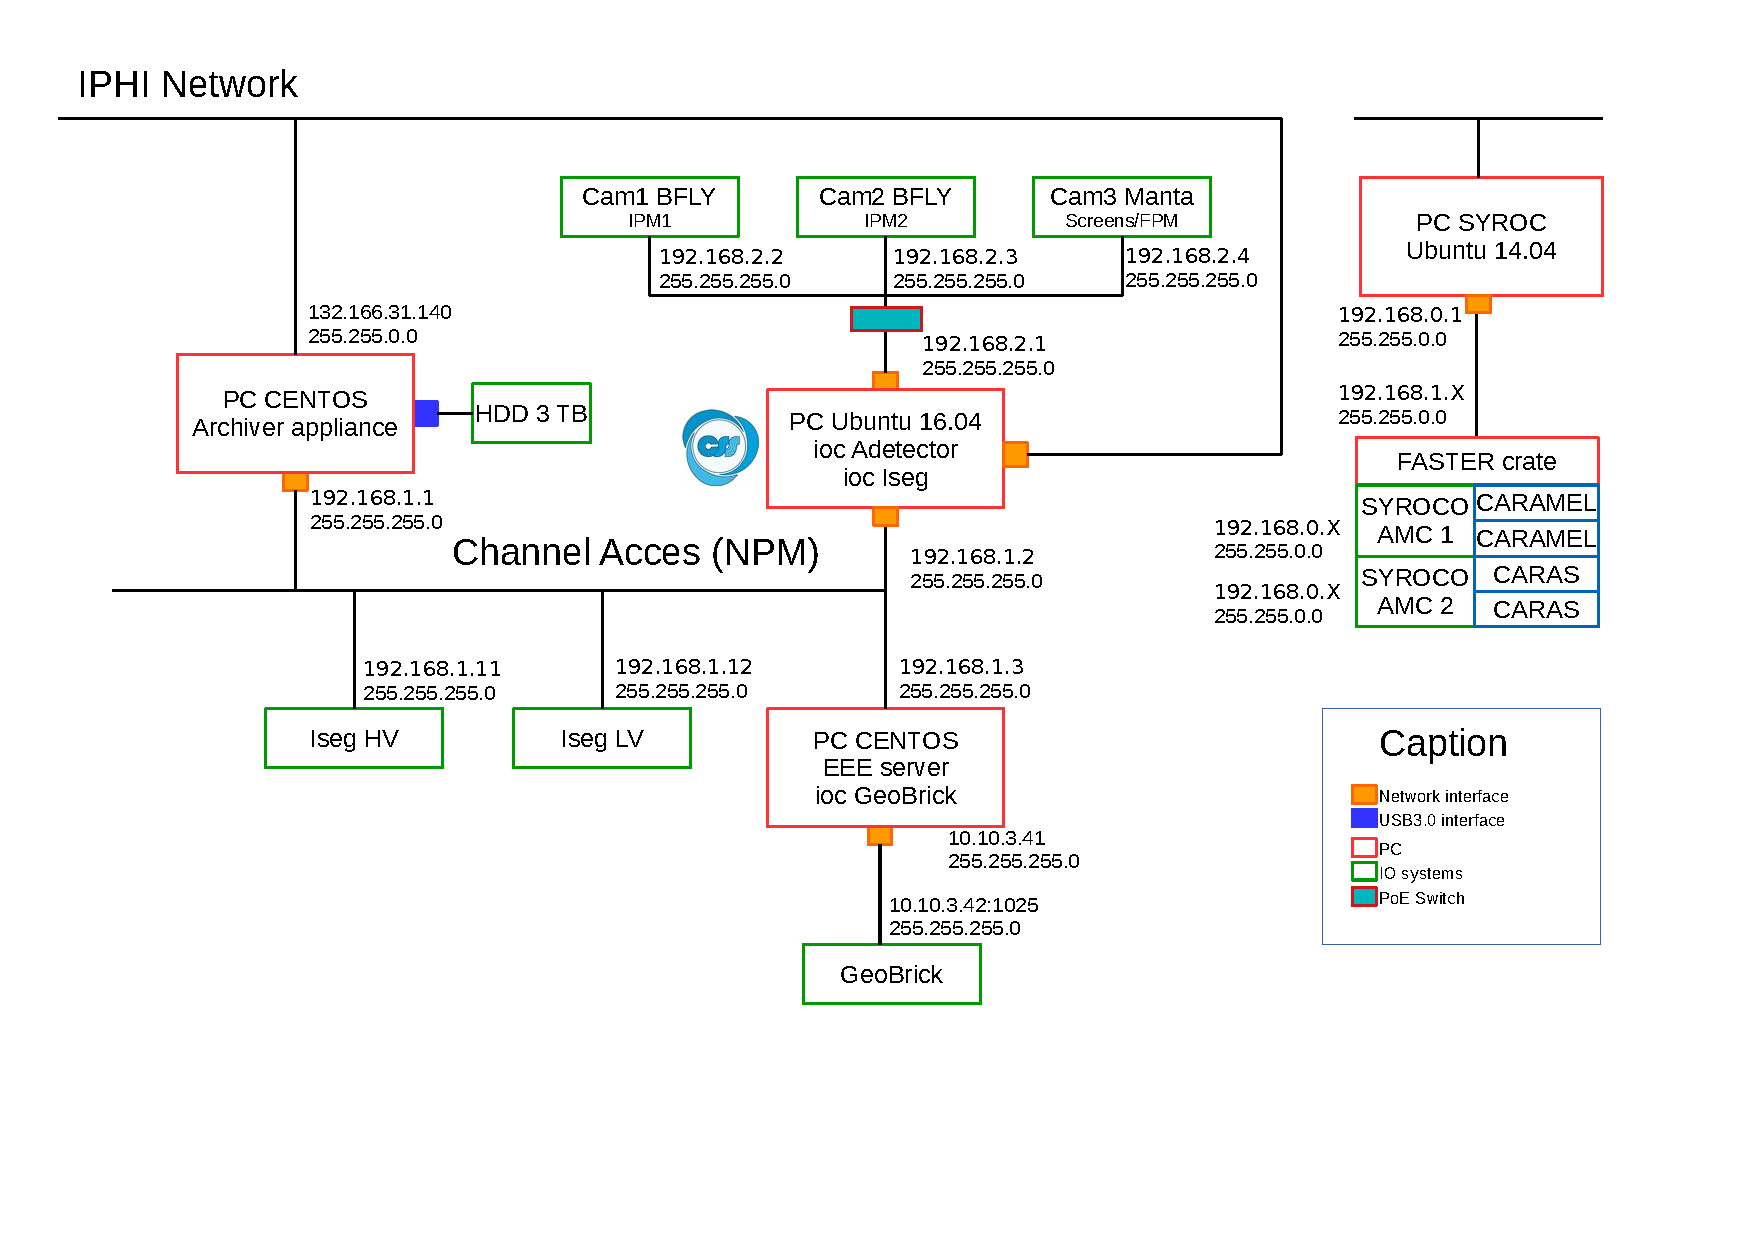
\includegraphics[width=\textwidth]{04_IPHI_Test/figures/fig000_EPICS_IPHI.pdf}
	\end{center}
	\caption[EPICS network setup during beam tests]{EPICS network setup during beam tests.}
	\label{chap4:EPICS_IPHI}
\end{figure}


  \subsection{Test bench}
  A test bench has been also developed in order to test the prototypes. The bench can be split into two different independent parts.

  The first part (upstream) is roughly similar to the \acrshort{ess} \acrshort{lwu} chamber (scale 1) on which two \acrshort{ipm}s can be inserted. The idea is to be close to the \acrshort{ess} conditions in term of high voltages and electrical fields. The second part (downstream) offers one more \acrshort{ipm} slot and two viewports for reference measurements in order to compare with the \acrshort{ipm} ones. Fig. \ref{chap4:Testbench} is a technical drawing of the test bench. One can see the resemblance of the upstream part with the \acrshort{lwu} vessel previously shown in Fig. \ref{chap3:LWU_Cryo} and \ref{chap3:COMSOL_LWU}.


  The \acrshort{ipm}s can be mounted independently in Y or X directions thanks to their design, thus it is even possible to measure the same transverse profile with all three \acrshort{ipm}s.

  \begin{figure}[!ht]
	\begin{center}
		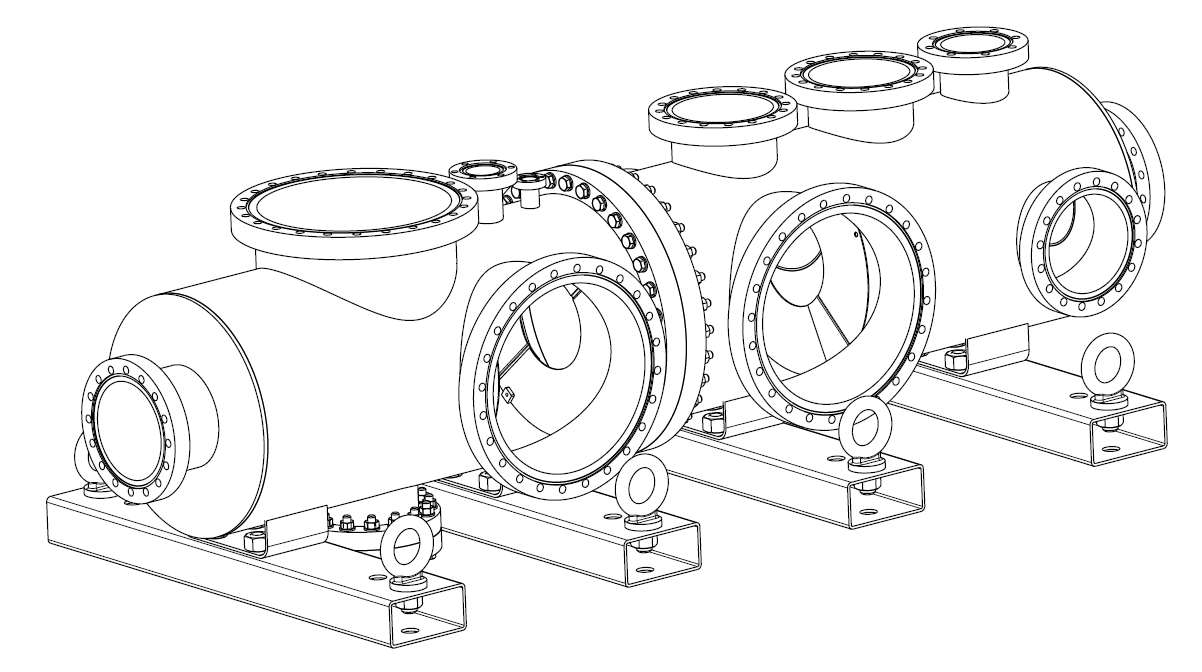
\includegraphics[width=\textwidth]{04_IPHI_Test/figures/fig000_Testbench.png}
	\end{center}
	\caption[IPM test bench]{IPM test bench. Left part is the LWU-like vessel
	while right part add more viewports for testing purposes.}
	\label{chap4:Testbench}
\end{figure}


  The test bench is pumped by 3 turbomolecular pumps with an average pumping speed of about $150\,\mathrm{L/s}$ at 3 different locations along the bench. The vessel can be baked using a heating system. The objective is to reach quickly the minimal vacuum level required to operate. Thus, during the tests it is possible to modify the \acrshort{ipm}s without sacrificing too much beam time. The whole system reaches a vacuum level of $1\cdot 10^{-7}\,\mathrm{mbar}$ in about ten hours (one night) after an intervention. An RGA and vacuum gauges monitor the vacuum level as close as possible to the \acrshort{ipm}s.

  \subsection{Reference measurement}
  \label{chap4:sec:ref}
  We carried out reference measurements for diagnosing possible issues on the prototypes and to allow a complete comparison with the prototypes, giving more confidence on the measurement. Two methods have been foreseen and implemented for this purpose.

  The first method uses scintillator screens, which is interceptive. The screens are mounted on a racket that can be inserted into the beam using a translator controlled remotely through a GEO BRICK controller. Three scintillator screens have been kindly provided by our colleagues at Saclay. Table \ref{chap4:tab_ecran} sums up the main characteristics of each screen.
  % and Fig \ref{chap4:fig_ecran} shows the three screens on a support.

  \begin{table}[ht]
	\centering
	\caption[]{Properties common semiconductors used as radiation detector.}
	\label{chap3:semiconductor}
	\begin{tabular}{llll}
    \toprule
    Property & $\mathrm{Prelude}420$ $(Lu^{1.8}Y.^{2}SiO^{5}:Ce)$ & $\mathrm{YAG:Ce}$ & $\mathrm{CdTeZn}$ \\
    \midrule
    Density &  &  &  \\
    Light yield &  &  &  \\
    Typical wavelength &  & & \\
		\bottomrule
	\end{tabular}
\end{table}

  The second system foreseen is a Fluorescence Profile Monitor (FPM). This system is developed by our \acrshort{ess} colleagues, indeed it will be the future \acrshort{npm} of the \acrshort{ess} MEBT. The \acrshort{fpm} relies on an Image Intensifier (\acrshort{ii}) and a \acrshort{cmos} camera.
  Such an image intensifier is made of a photocathode, converting photons in electrons, which are then amplified by a single or a double \acrshort{mcp} stage, before to be converted back into photons through a phosphor screen. The high sensitivity of an II allows to detect the unique photo-electron. The \acrshort{fpm} is a totally non invasive method.

  % An intensify image is a device that amplify visible photons. A photocathode on its input converts a incident photon into electrons. These electrons are then amplified by a single or double stages \acrshort{mcp} and converted back into photons using a phosphor screen. Finally, a camera records the amplified image on the back of the phosphor screen. An II may detect a single photon as long as the incident photon is converted by the photocathode. However the information of the wavelength cannot be recover. The \acrshort{fpm} is a totally non invasive method.

  %\begin{wrapfigure}{r}{0.3\textwidth}
  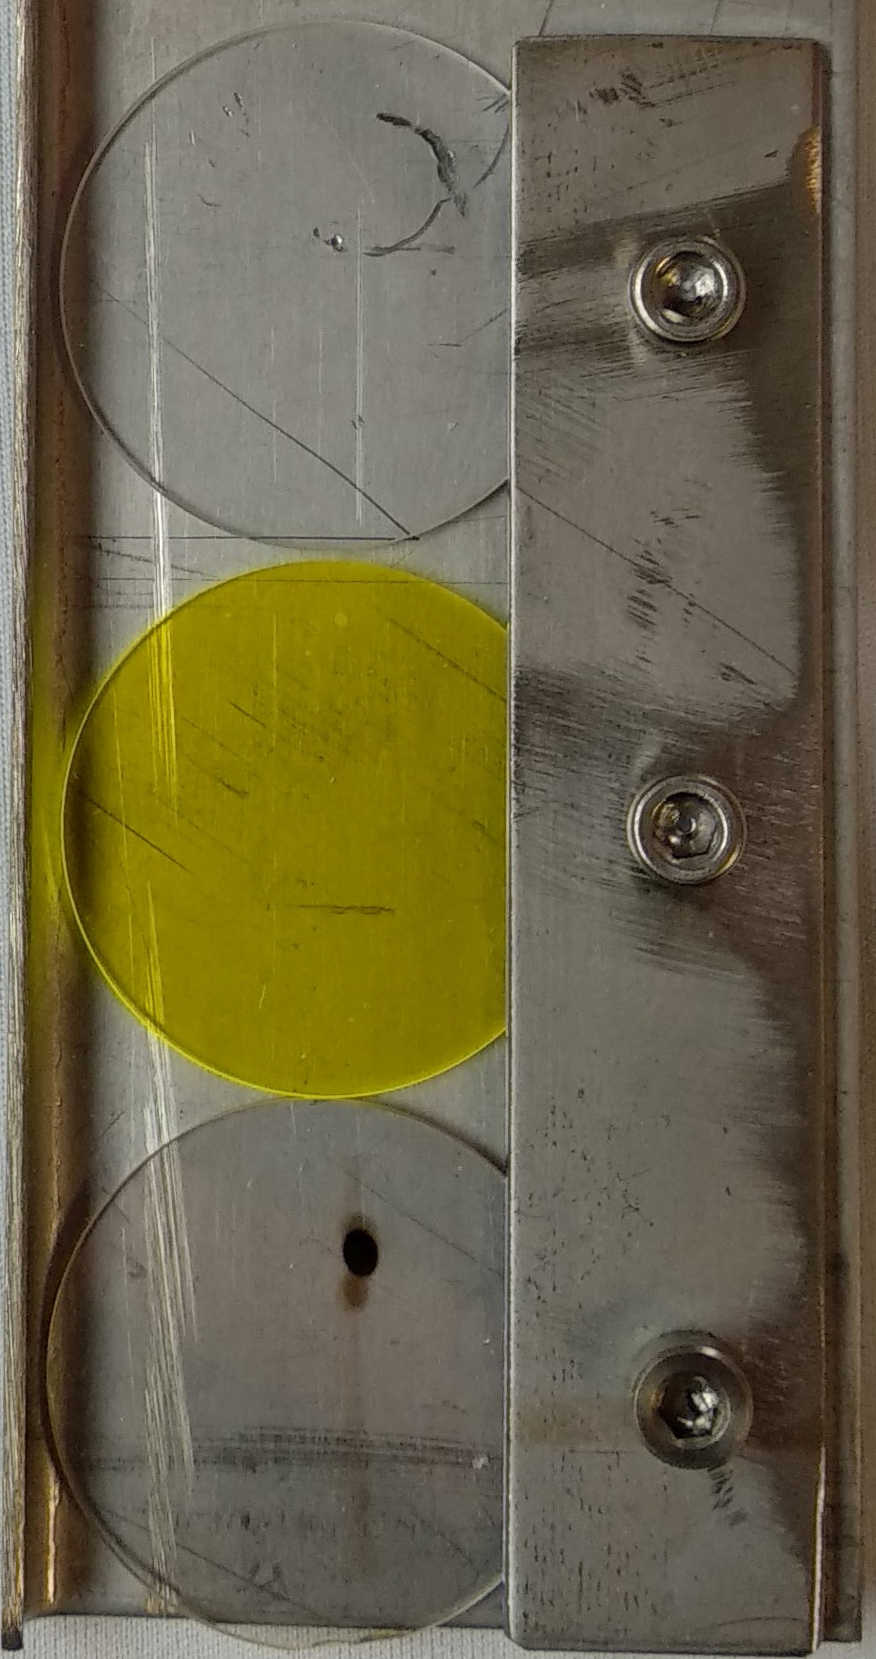
\includegraphics[width=0.3\textwidth]{04_IPHI_Test/figures/fig000_ecran.jpg}
  \caption[Picture of scintillator screen]{Picture of scintillator screen: Prelude420 (top), YAG:Ce (middle) and BGO (bottom).}
	\label{chap4:ecran}
\end{wrapfigure}


  \section{IPHI and test campaigns}

  We had the opportunity to test twice our prototypes at the \acrshort{iphi} accelerator. In the following sections, the accelerator and the two campaigns are briefly introduced. Pictures of the installation are shown in Fig. \ref{chap4:IPHI_tb}.

  \subsection{IPHI accelerator}
  \acrshort{iphi} is a high intensity linear proton accelerator located at CEA/Saclay.
  The project started in the late 90's \cite{Beau2000} but protons were accelerated up to $3\,\mathrm{MeV}$ only in April 2016 \cite{Gobin2016}.

  \begin{figure}[!ht]
  \begin{center}
    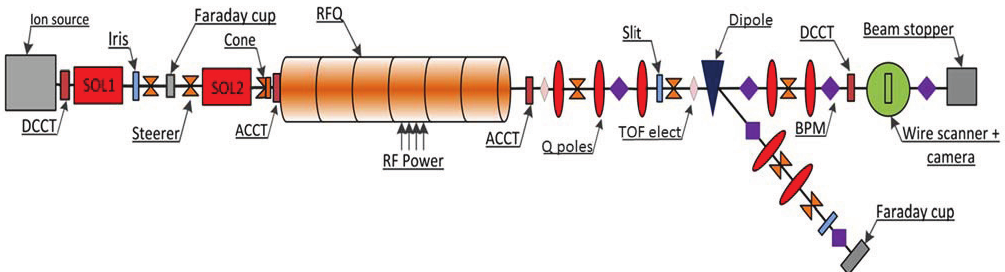
\includegraphics[width=\textwidth]{04_IPHI_Test/figures/fig000_IPHI_view.png}
  \end{center}
  \caption[Schematic view of IPHI accelerator]{Schematic view of the IPHI accelerator. The layout is almost up to date except that the slits have been removed. Our test bench was installed just after the last BPM on the deviated line.
    There is no other beam profiler measurement on this line.}
  \label{chap4:IPHI_view}
\end{figure}

  Proton plasma is created by an electron cyclotron resonance source (ECR), and transported toward a radio frequency quadruple (\acrshort{rfq}) by a low energy beam transport line (LEBT).
  An iris, at the source exit, ensures a fine tuning of the current, and two solenoids focus and filter the beam before the injection into the RFQ.
  Then, the protons are accelerated up to $3\,\mathrm{MeV}$ and bunched at a frequency of $352\,\mathrm{MHz}$.
  A medium energy beam transport line (MEBT), downstream from the RFQ, contains focusing elements, steerers and beam diagnostics.
  A bit further, the dipole magnet can distribute the protons over two beam lines.

  The main line has a dedicated beam stop of $300\,\mathrm{kW}$, allowing the commissioning of the accelerator at high intensity and duty cycle.
  The secondary line is more modular but restricted to beam at lower intensity and duty cycle (few hundred Watt).
  This line is open for external user experiments.
  We were, with the \acrshort{nblm} team, one of the first experiments on the deviated line \cite{Senee:IPAC2018-TUPAF016}.

  % TODO: Parler de linac4 ?
  Fig. \ref{chap4:IPHI_view} shows a schematic view of the \acrshort{iphi} accelerator, and Table \ref{chap4:IPHI_carac} sums up the main differences between \acrshort{iphi} and \acrshort{ess}. Even if IPHI does not have the same characteristics, it is close to our laboratory and very convenient for testing purpose. The extrapolation from IPHI to ESS conditions will be done as soon as the following product $I_{beam}\,\times\,P_{gas}\,\times\sigma(E_{beam})$ is kept constant for both facilities.

  \begin{table}[!h]
  \centering
  \caption[Comparison between IPHI and ESS accelerators]{Comparison between IPHI and ESS accelerators.}
  \label{chap4:IPHI_carac}
  \begin{tabular}{lll}
    \toprule
                         & IPHI accelerator                                  & ESS accelerator                \\
    \midrule
    Energy               & $3\,\mathrm{MeV}$                                 & $2\,\mathrm{GeV}$              \\ \hline
    Max current          & $100\,\mathrm{mA}$                                & $62.5\,\mathrm{mA}$            \\ \hline
    Max pulse duration   & up to DC                                          & $2.86\,\mathrm{ms}$            \\ \hline
    Max pulse repetition & -                                                 & $14\,\mathrm{Hz}$              \\ \hline
    Vacuum range         & $5\cdot10^{-7}$ to $1\cdot10^{-8}\,\mathrm{mbar}$ & $1\cdot10^{-9}\,\mathrm{mbar}$ \\
    \bottomrule
  \end{tabular}
\end{table}

  \subsection{Overview of the two test campaigns}
  In this section, we want to introduce the story behind our two test campaigns, and give an overview of the issues we faced.

  \begin{figure}[!ht]
	\begin{subfigure}{0.5\textwidth}
		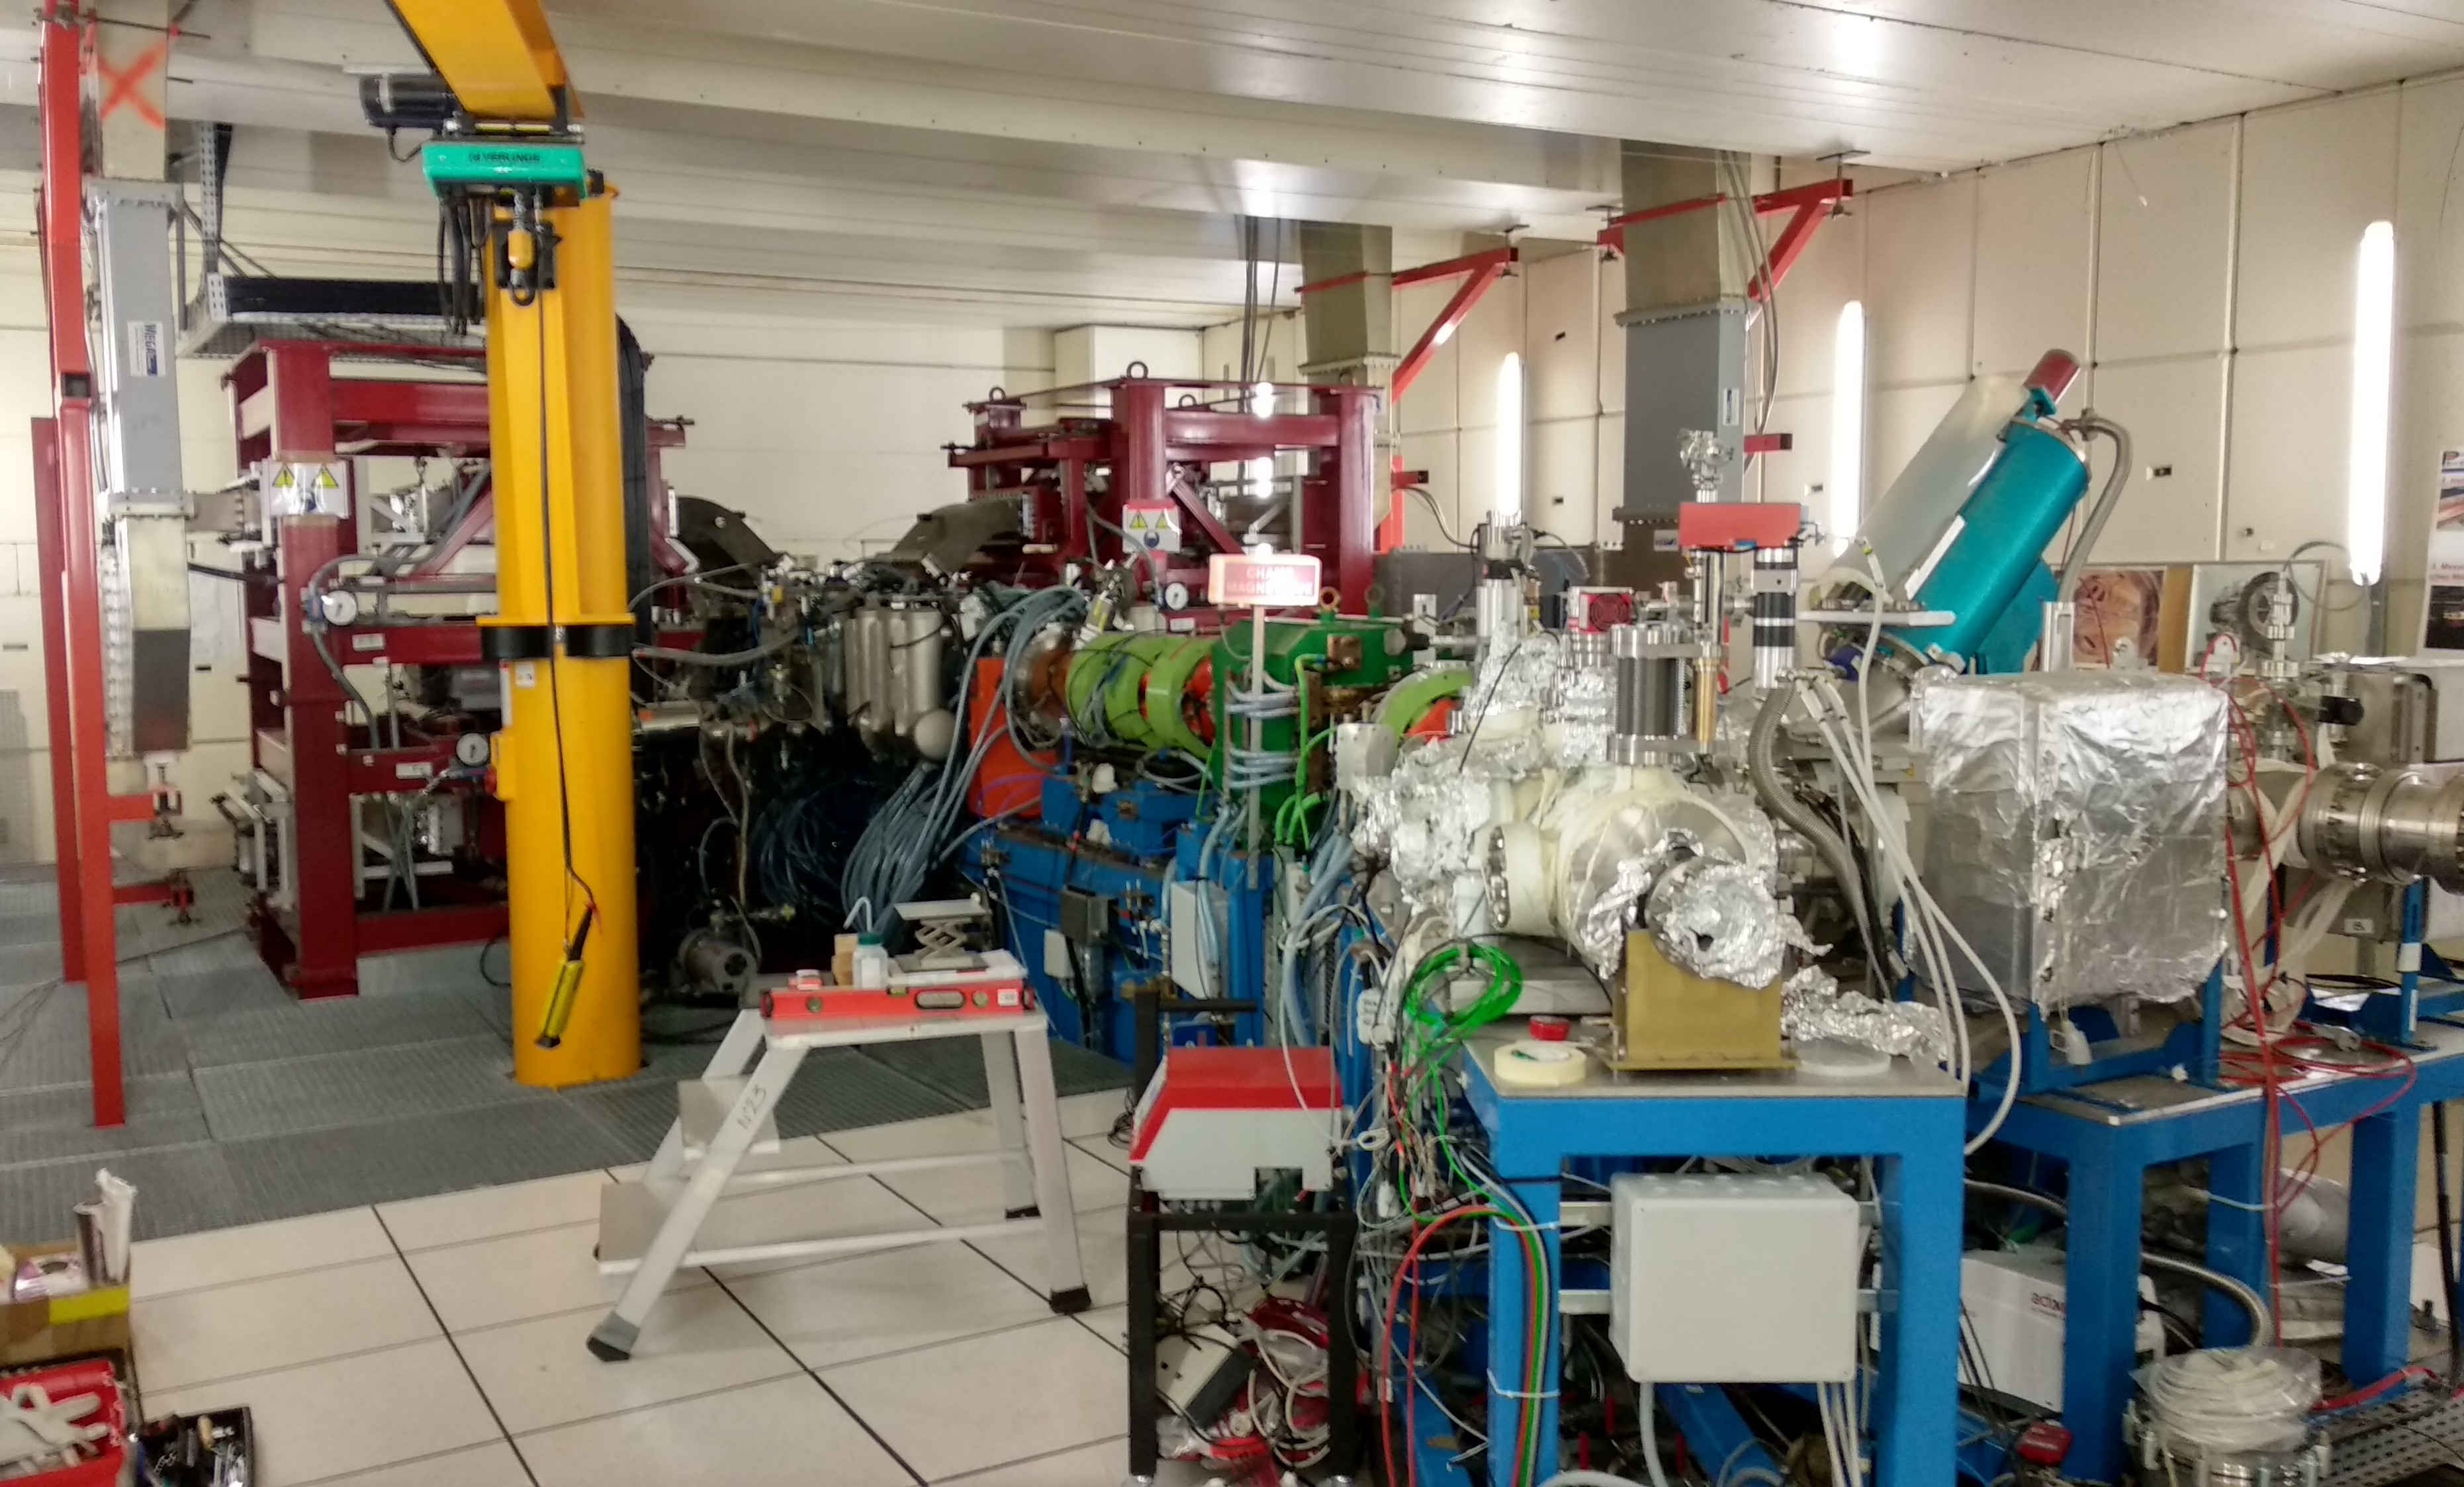
\includegraphics[width=\textwidth]{04_IPHI_Test/figures/fig000_IPHI_tb1.jpg}
		\caption{The casemate of IPHI. The test bench is visible in foreground}
		\label{}
	\end{subfigure}
	~
	\begin{subfigure}{0.5\textwidth}
		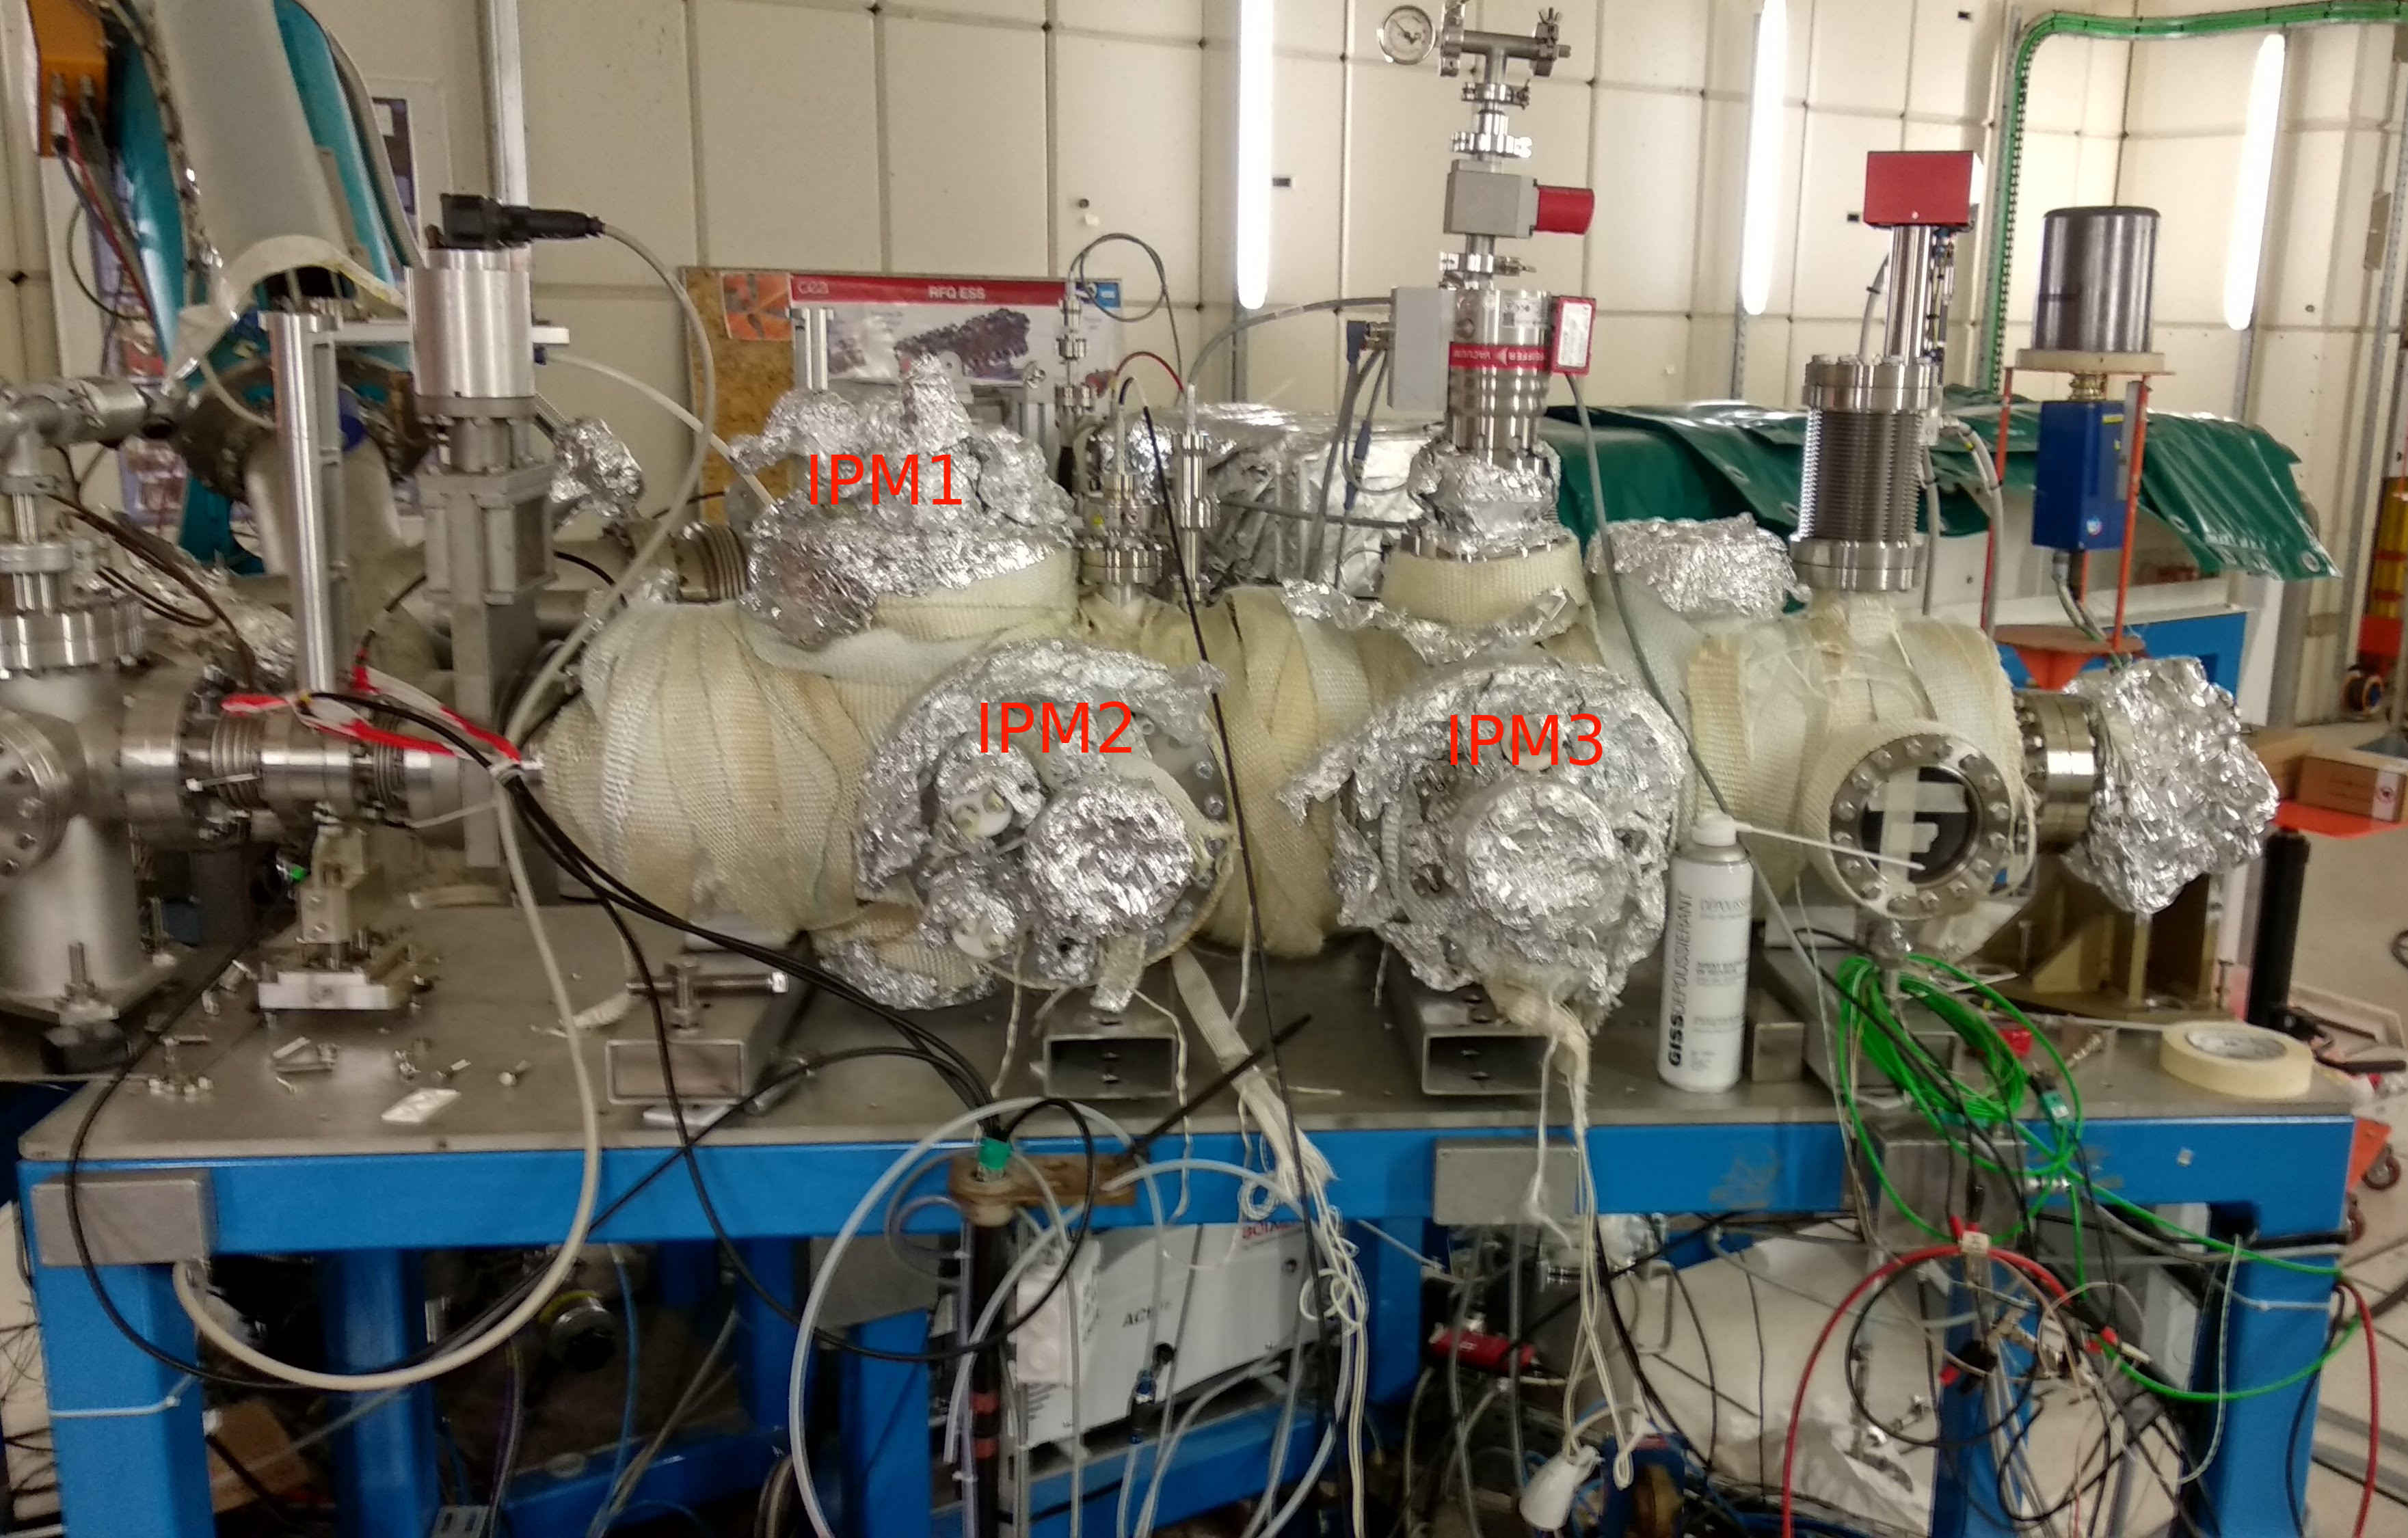
\includegraphics[width=\textwidth]{04_IPHI_Test/figures/fig000_IPHI_tb2.jpg}
		\caption{The test bench fully equipped.}
		\label{}
	\end{subfigure}
	\caption[The test bench installed at IPHI accelerator]{Th test bench installed at IPHI accelerator.}
	\label{chap4:IPHI_tb}
\end{figure}


  The prototypes were not ready for the beginning of the first campaign.
  Hence, they were debugged on site, and we encountered many technical problems (sparks, readout synchronization).
  We finally got our first profile after some fixes on our prototypes, and by reducing the maximum operating voltage.
  However, our prototypes were not able to measure the beam profile on demand, working sporadically, and we observed strange artifacts on the profiles.
  We solved this problem by asking a fine tuning of the beam parameters to a beam physicist.
  We became even more confident with our detectors when \acrfull{bpm} systems were switched on allowing a comparison with our measurements, see section \ref{chap4:sec:Position}.


  Just after the first campaign the detectors were improved by minor changes on the HV connection design. Therefore, the decision was made to perform a second test campaign at \acrshort{iphi}.
  The results of the first campaign were confirmed and improved during this second one.
  The beam time was shared between four experiments, with different requirements on the beam parameters.
  Unfortunately, the schedule was not respected due to technical problems and other external issues, so
  we had to manage our tests daily and get along with the other experiments.
 For the above reasons, we did not manage to perform all the advanced tests we had planned to do.
  Table \ref{chap4:IPHI_campaign} summarizes our two beam test campaigns

  \begin{table}[!h]
  \centering
  \begin{tabular}{ccc}
    \toprule
                  & First campaign      & Second campaign     \\
    \midrule
    Starting date & 19/02/2018          & 14/09/2018          \\
    First profile & 01/03/2018          & 14/09/2018          \\
    Ending date   & 13/04/2018          & 26/10/2018          \\
    IPM 1         & Linear strips (Y)   & Gaussian strips (X) \\
    IPM 2         & Hamamatsu MCP (Y)   & Photonis MCP (Y)    \\
    IPM 3         & Gaussian strips (Y) & Linear strips (Y)   \\
    \bottomrule
  \end{tabular}
  \caption[Summary of the two campaigns]{Summary of the two campaigns.}
  \label{chap4:IPHI_campaign}
\end{table}


  \section{Processing data}
  In the following sections, the data processing is briefly explained based on several methods. Each method has its own characteristics, so the data processing is different depending on the \acrshort{ipm}. The term beam size refers to the $\sigma_{beam}$ of the beam. The error bars in the following plots are given for a confidence level of $95\,\mathrm{\%}$. This assumes that the variation follows a normal distribution.

  \subsection{Processing camera}

  The optical \acrshort{ipm} gives directly an image of the beam in longitudinal and transverse directions. Thanks to EPICS and AreaDetector, all images and related acquisition information are packed together in an \acrshort{hdf}5 file. The processing of data is done with different Python packages \cite{NumPy2011,SciPy2019,Hunter2007}. In a first step, dead pixels are removed: the standard deviation of the image is computed and each deviating pixel is smoothed by a convolution filter ($3\times3$ kernel). The algorithm works well if two dead pixels are not neigbours, otherwise higher order kernel must be used. Then, the image is cropped to a region of interest i.e. the active surface of the \acrshort{mcp}. If necessary, the image is filtered in the frequency domain via a Fast Fourier Transform (\acrshort{fft}) \cite{Burrus2012}. \acrshort{fft} filtering is a very efficient method when the images have many recurring pattern that are even visible by a human eye. At \acrshort{ess}, more advanced methods like wavelets \cite{Burrus1997,bultheel2014} may be more suitable for filtering patterns with some spatial dependencies. Indeed, the images may have some discrete spots rather than a continuous image\footnote{More details in section \ref{chap4:sec:MCPess}.}. Note that beam images are quite parsimonious in the frequency domain. The profile is reconstructed by summing all pixels in the longitudinal direction. An example of an almost raw image is visible in Fig. \ref{chap4:image_beam}.

  \begin{figure}[!ht]
	\begin{center}
		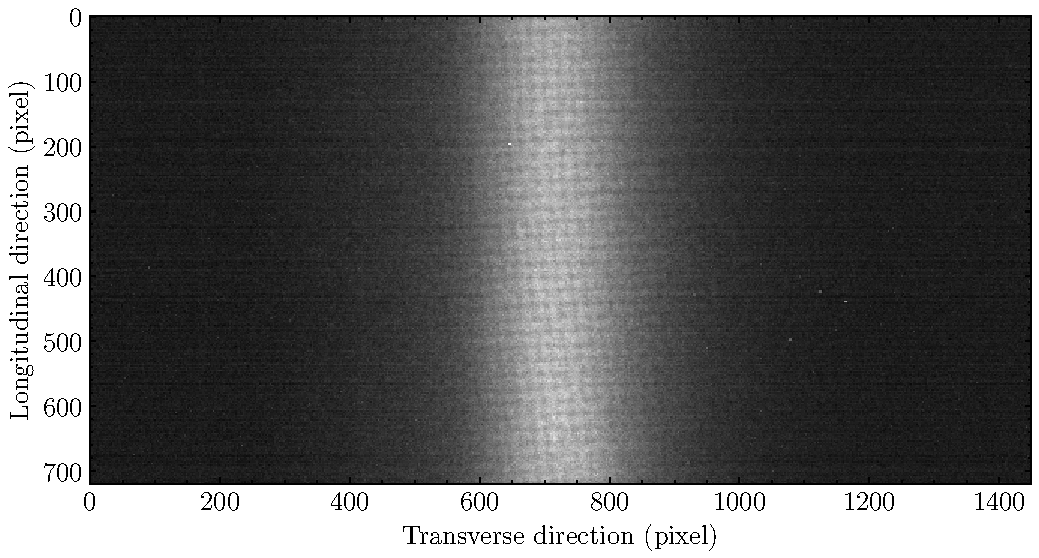
\includegraphics[width=\textwidth]{04_IPHI_Test/figures/fig000_image_beam}
	\end{center}
	\caption[An example of a beam image recorded by the camera]{An example of a beam image recorded by the camera. The image has just been cropped to a region of interest. The shadow of the grid is visible.}
	\label{chap4:image_beam}
\end{figure}


  \subsection{Processing strip}
  The processing of data from strips is completely different and more complex. Indeed only a small part of the recorded signal is meaningful since the chips integrate continuously. The duration of the beam pulse was always short during the tests (from $50\,\mathrm{\mu s}$ to $1\,\mathrm{ms}$), therefore only a small amount of data is really useful.
  \begin{figure}[!ht]
  \begin{subfigure}{0.5\textwidth}
    \includesvg[width=\textwidth]{04_IPHI_Test/figures/fig000_strips_signal_a.svg}
    \caption{Full signal over a 45 sec.}
    \label{}
  \end{subfigure}
  ~
  \begin{subfigure}{0.5\textwidth}
    \includesvg[width=\textwidth]{04_IPHI_Test/figures/fig000_strips_signal_b.svg}
    \caption{Zoom on one pulse beam pulse.}
    \label{}
  \end{subfigure}
  \caption[Example of charge signal recorded on one strips]{Example of charge signal recorded on one strips.}
  \label{chap4:strips_signal}
\end{figure}


  The data are processed as follows with ROOT\cite{Brun1997,Antcheva2009} routines. First, the pedestal of each strips is subtracted. If $N$ successive points are above a given threshold, then the pulse is considered as triggered. A pulse is detected when the previous condition is met on several strips at same time. Finally the successive $N$ integrations are summed giving the charge collected for one pulse. For Gaussian strips the charges are weighted according to the size of the strip.

  An example of a raw signal is given in the Fig. \ref{chap4:strips_signal}. On the left hand side, one can see the signal recorded during $45\,\mathrm{s}$. Each peak corresponds to the passage of the beam. The signal for one pulse is visible on the right hand side.


  \subsection{Processing scintillator screen data and review of the reference measurements}

  Scintillator screens can only operate at low duty cycles, typically few mA and few hundred $\mu$s. Even under these conditions, the beam destroyed two of the three screens. The signal is so strong that the camera in front of the screen is completely saturated, as well as the camera of the optical \acrshort{ipm} one meter away. Measurements with the scintillator screens are only possible if a neutral density (ND) filter is set in front of the lens. The signal from the scintillating screen completely overlaps with the one from the phosphorus screen and since we use monochromatic camera, there is no way to recover the beam profile from the optical \acrshort{ipm}. For the strips \acrshort{ipm} the working conditions are already too low for a correct measurement. Therefore, it is not possible to compare the \acrshort{ipm} beam profiles with the scintillating screens in real time.
  \begin{figure}[!ht]
	\begin{subfigure}[t]{0.3\textwidth}
		\includesvg[width=\textwidth]{04_IPHI_Test/figures/fig000_ScreenBeam_a}
		\caption{Image on screen}
		\label{}
	\end{subfigure}
	~
	\begin{subfigure}[t]{0.3\textwidth}
		\includesvg[width=\textwidth]{04_IPHI_Test/figures/fig000_ScreenBeam_b}
		\caption{Projection on $x$ axis}
		\label{}
  \end{subfigure}
  ~
  \begin{subfigure}[t]{0.3\textwidth}
		\includesvg[width=\textwidth]{04_IPHI_Test/figures/fig000_ScreenBeam_c}
		\caption{Projection on $y$ axis}
		\label{}
  \end{subfigure}
	\caption[Beam profile measurement with the $Y_{3}Al_{5}O_{12}(Ce)$ screen]{Beam profile measurement with the $Y_{3}Al_{5}O_{12}(Ce)$ screen.}
	\label{chap4:ScreenBeam}
\end{figure}

  Fig. \ref{chap4:ScreenBeam} shows an example of a profile measurement recorded on the $Y_{3}Al_{5}O_{12}(Ce)$ screen. The processing is almost the same as the optical \acrshort{ipm}: hot pixels are corrected and the images are cropped. Then, a homography \cite{szeliski2010,opencv_library} is performed to correct the orientation of the screens. The measurement of the beam size is quite complicated because the baseline of the profile is not straight, therefore the fits have a very poor quality. One can see that the profile is quite wide in the $x$-plane because of the dispersion due to the dipole.
  %During the second campaign the dispersion was reduced by a small aperture collimator located downstream the deviation dipole.

  The conditions are also not favorable for measurements with \acrshort{fpm}s. The viewports are very close to the beam dump and when this stops beam particles stray light is emitted. The vacuum chamber (and the entire accelerator) allows light to propagate easily due to reflections on 304L steel. The vacuum is quite low so the expected fluorescence signal will be even weaker. Increasing the beam intensity does not help since the parasitic light from the beam dump becomes more significant.
  Our concerns were confirmed when we added a sleeve with a black coating to shield the \acrshort{fpm}s field of view from the rest of the vessel. The parasitic light is shown in Fig. \ref{chap4:FPM}. All the attempts to minimize this effect remained unsuccessful.

  \begin{figure}[!ht]
	\begin{center}
		\includesvg[width=0.5\textwidth]{04_IPHI_Test/figures/fig000_FPM}
	\end{center}
	\caption[Image recorded with the FPM system.]{Image recorded with the FPM system. The light coming from outside of the sleeve doesn't permit a correct measurement.}
	\label{chap4:FPM}
\end{figure}


  \section{Beam environnement characterization}
  First of all, it is necessary to present the experimental conditions under which our detectors have been characterized. One of the major problems encountered during these tests was the lack of information about the beam. The two types of diagnostics available at \acrshort{iphi} on the deviated line are current monitors and \acrshort{bpm}s, whose calibration is uncertain. During the first weeks of the test campaign, it was impossible to know if the strange beam position oscillations observed were due to the beam or to the detectors themselves. The next sections show the tests carried out in order to understand the origin of the instabilities

  \subsection{Vacuum analysis}
  \label{sec4:vacuum}
  Understanding the vacuum conditions is very important in order to correctly extrapolate our results to ESS conditions. During the tests, the vacuum parameters were recorded in real time \footnote{The vacuum gauge can provide a measurement at every pulse whereas a full RGA scan takes around two minutes}. However, neither the RGA, nor the vacuum gauge were calibrated. It is assumed that the RGA provides a qualitative information about the proportions of each specie in the residual gas, whereas the vacuum level is given more precisely by the vacuum gauge.

  We measured two main types of RGA spectra as shown in Fig. \ref{chap4:vacuum_rga}. The left one is obtained when the chamber had not been baked or after a water contamination. As a consequence, the water peak dominates and the pressure is in the range of $10^{-7}\,\mathrm{mbar}$. After few days of pumping or after drying, the RGA spectra tend towards the second case, on the right. In this case the vacuum level is about $10^{-8}\,\mathrm{mbar}$ and hydrogen is the main molecular specie. One can see some quite heavy elements on the two spectra, possibly oil residues. Indeed one of our turbo pumps was contaminated with oil from its old primary pump.

  \begin{figure}[!ht]
  \begin{subfigure}[t]{0.5\textwidth}
    \includesvg[width=\textwidth]{04_IPHI_Test/figures/fig000_vacuum_rga_a}
    \caption{An RGA spectrum dominated by water peaks.}
    \label{chap4:vacuum_rga_b}
  \end{subfigure}
  ~
  \begin{subfigure}[t]{0.5\textwidth}
    \includesvg[width=\textwidth]{04_IPHI_Test/figures/fig000_vacuum_rga_b}
    \caption{An RGA spectrum after few days of pumping or baking.}
    \label{chap4:vacuum_rga_a}
  \end{subfigure}
  \caption[Two types of RGA spectra recorded during the tests]{Two types of RGA spectra recorded during the tests.}
  \label{chap4:vacuum_rga}
\end{figure}


  When the beam is running, the pressure increases slightly as well as the amplitude of all the peaks in the RGA spectrum. We suppose that theses effects are mainly due to the heating of the beam dump. In the same way, the pressure increases when the resistance chains are fed, probably due to the Joule effect. On some RGA spectra, the hydrogen peak is subject to overshoots when the beam is running.

  \subsection{Beam position}
  \label{chap4:sec:Position}

  The first observation we made on the profile measurements was the significant variation of the beam position between two pulses. At first, we thought to an electrostatic charge and discharge phenomenon, that induced beam position oscillation. However, this hypothesis was discarded when finally the \acrshort{bpm} system was started. For the first time, we were able to compare our measurements with another device. Fig. \ref{chap4:BPMvsIPM} shows the position of the beam recorded by \acrshort{ipm} and a \acrshort{bpm} on a time scale of about one hour. The big sharp transitions are the consequences of beam moving under the electrostatic steerer scans. However, there are quite a few smaller variations between two steerer steps. A variation exceeding $2\,\mathrm{mm}$ ($5\,\mathrm{\%}$ of our readout size) can be observed from pulse to pulse. The \acrshort{ipm} position is the center of the gaussian fit of the profile; this nice correlation started giving us confidence in our monitoring systems.
  %This is not a profile comparison but the same beam instabilities are visible on both devices.

  \begin{figure}[!ht]
	\begin{center}
		\includesvg[width=\textwidth]{04_IPHI_Test/figures/fig000_BPMvsIPM}
	\end{center}
  \caption[Beam position over the time measured with the BPM and the IPM]
  {Beam position over the time measured with the BPM and the IPM.
  A steerer has been used to move the beam (step transitions).
  However, small variations between two steerer steps were not expected. 
  Positions were directly extracted from IOCs without any processing.}
	\label{chap4:BPMvsIPM}
\end{figure}


  This is a major issue since \acrshort{mcp}s have a good space resolution, but we are not allowed to fully benefit of this feature. Indeed, all our measurements have been affected by those parasitic variations and therefore the level of confidence on the measurement is reduced. The histograms of beam size and position over 480 consecutive pulses are reported in Fig. \ref{chap4:hist_variation}. 
  \begin{figure}[!ht]
  \begin{subfigure}[t]{0.5\textwidth}
    \includesvg[width=\textwidth]{04_IPHI_Test/figures/fig000_hist_variation_a.svg}
    \caption{Histogram of positions.}
    \label{}
  \end{subfigure}
  ~
  \begin{subfigure}[t]{0.5\textwidth}
    \includesvg[width=\textwidth]{04_IPHI_Test/figures/fig000_hist_variation_b.svg}
    \caption{Histogram of sizes.}
    \label{}
  \end{subfigure}
  \caption[Histograms of the beam positions and sizes for 480 consecutive pulses]{Histograms of the beam position and size for 480 consecutive pulses.}
  \label{chap4:hist_variation}
\end{figure}


  One can see that both distributions are asymmetric and have a similar shape. The linear regression between size and position has been calculated from several runs and shows a non-zero slope. On the other hand the correlation factor between size and position is not so high usually and varies between $0.5$ and $0.8\,\mathrm{mm}$ from run to run.
  Anyway, these uncertainties can be seen as systematic errors, thus measurement errors may be calculated and reduced quadratically from the oscillating components!

  The main explanation given by \acrshort{iphi} experts about theses variations is that the beam is more unstable when the pulse beam is shorter. However, we did not have time to confirm this hypothesis.

  \subsection{Beam current}
  \label{chap4:sec:current}
  At \acrshort{iphi} the current is finely adjustable thanks to the iris located at the source exit; \acrshort{iphi} has been designed to work with a continuous beam up to $100$ $\mathrm{mA}$. To be in conditions close to those of \acrshort{ess} in term of counting rates, the current and duration of the pulse must be lowered. Varying the beam current is very important because it allows to check many properties of the detector. However, the shape of the \acrshort{iphi} beam changes greatly with current. This phenomenon is illustrated in Fig. \ref{chap4:ex_beam_profile_a} and \ref{chap4:ex_beam_profile_b}. When the currents are high, the beam looks like a Gaussian with one of its shoulders with a longer tail. At medium and low current, the size of the beam decreases as well as its amplitude. However, a kind of halo appears and this becomes more and more important as the current decreases. At very low current the beam core disappears completely and only the halo remains.

  \begin{figure}[!ht]
  \begin{subfigure}[t]{0.5\textwidth}
    \includesvg[width=\textwidth]{04_IPHI_Test/figures/fig000_ex_beam_profile_a.svg}
    \caption{At high current the beam looks almost Gaussian.}
    \label{chap4:ex_beam_profile_a}
  \end{subfigure}
  ~
  \begin{subfigure}[t]{0.5\textwidth}
    \includesvg[width=\textwidth]{04_IPHI_Test/figures/fig000_ex_beam_profile_b.svg}
    \caption{At low beam current, the beam shows a narrow peak on the top of a large halo.}
    \label{chap4:ex_beam_profile_b}
  \end{subfigure}
  \caption[Influence of the beam current on the beam shape.]{Influence of the beam current on the beam shape.}
  \label{chap4:ex_beam_profile}
\end{figure}


  This causes a problem for beam shapes comparisons at different beam intensities. So, how to quantify the beam size? Several methods have been considered. One can simply calculate the mean value and standard deviation of the profile distribution, but the results are strongly biased by the beam position and the asymmetric shape of the profile. A more advanced method consists in performing a least squares curve fitting of the profile with a Gaussian function for recovering the estimated sigma. This method works quite well at high currents but at low currents the halo prevents the beam from performing a correct fitting. To overcome this issue, a second Gaussian function can be added to the fitting routine. The double fit succeeds in correctly modeling the two components. However, double fits may modelize almost any beam shape and the fitting results are difficult to verify automatically. The method becomes very unstable for high currents. This is why it must be limited to low currents. The last alternative is to use the full width at half maximum (FWHM). Assuming that the beam is more or less Gaussian, the sigma can be calculated as follow $\sigma = \frac{FWHM}{\sqrt{2ln(2)}}$. FWHM computation is also less complicated than least squares fitting.

  \begin{figure}[!ht]
  \begin{subfigure}[t]{0.5\textwidth}
    \includesvg[width=\textwidth]{04_IPHI_Test/figures/fig000_current_sweep_a}
    \caption{Integrated signal versus beam current. The blue curve represents the sum of the two components.}
    \label{}
  \end{subfigure}
  ~
  \begin{subfigure}[t]{0.5\textwidth}
    \includesvg[width=\textwidth]{04_IPHI_Test/figures/fig000_current_sweep_b}
    \caption{Sizes of the beam and halo versus beam current.}
    \label{}
  \end{subfigure}
  \caption[Influence of the beam current on the profile measurement.]{Influence of the beam current on the profile measurement.}
  \label{chap4:current_sweep}
\end{figure}


  On Fig. \ref{chap4:current_sweep}, the double fitting routine was used to monitor the evolution of both beam components. First, the phenomenon described above is clearly visible. At high current the signal tends towards a Gaussian shape, whereas at low current the double Gaussian model seems more realistic. Secondly, the amplitude of the signal is linear with the beam current. At high currents the input signal on the \acrshort{mcp} is by several orders of magnitude above the expected signal at \acrshort{ess}. This means that there will be no saturation at \acrshort{ess} with a single-stage \acrshort{mcp}.

  \subsection{Beam tuning}

  The beam tuning is also important to insure a correct measurement of the profile. The \acrshort{iphi} line contains many beam optics elements to control the beam transport. An incorrect adjustment of the beam has significant consequences on the quality of our measurements. Indeed, during the first weeks of testing, we could not get stable and reproducible measurements. An example is given in Fig. \ref{chap4:beam_tuning_a}. One can see that the profile is visible in the image, but with a kind of halo on the top. We have no explanation about the origin of this halo. This effect disappears completely when the beam is properly adjusted.

  The optimal parameters were found with the help of a beam physicist using the TraceWin software. In practice, the beam has been adjusted to have the lowest possible convergence all along the test bench. The beam size has been tuned to be close to ESS conditions (around few $\mathrm{mm}$) with the different quadrupoles (Fig. \ref{chap4:beam_tuning_b}). Once the beam was adjusted, all the parameters were frozen. This allowed us to measure the profile correctly.

  \begin{figure}[!ht]
  \begin{subfigure}[t]{0.5\textwidth}
    \includesvg[width=\textwidth]{04_IPHI_Test/figures/fig000_beam_tuning_a}
    \caption{A poorly beam tune leads to strange signal on the top of the image.}
    \label{chap4:beam_tuning_a}
  \end{subfigure}
  ~
  \begin{subfigure}[t]{0.5\textwidth}
    \includesvg[width=\textwidth]{04_IPHI_Test/figures/fig000_beam_tuning_b}
    \caption{The beam size can be set at different size thank to quadrupoles.}
    \label{chap4:beam_tuning_b}
  \end{subfigure}
  \caption[The beam must be finely tune in order to perform correct measurements]{The beam must be finely tune in order to perform correct measurements.}
  \label{chap4:beam_tuning}
\end{figure}


  %\input{04_IPHI_Test/figures/fig000_position_sweep}

  \section{IPM characterization}
  In the next sections the most common aspects of \acrshort{ipm}s are presented. The goal is to collect as much information as possible about the detectors and their limitations to prepare the final design. Most of the data presented below come from optical \acrshort{ipm}s, since many of the acquisitions done with the strips were polluted by strange electronics noises.

  \subsection{Beam size convergence}

  The extraction voltage is an important parameter of an IPM; if the electricl field is too low, then profiles will be distorted by the molecular thermal motion and beam space charge effects. Those effects can be compensated by increasing the electrical field in the cage. At a certain point, the beam size will start to converge to its real value. This behavior has been observed with both strip and optical IPMs.
  \begin{figure}[!ht]
  \begin{subfigure}[t]{0.5\textwidth}
    \includesvg[width=\textwidth]{04_IPHI_Test/figures/fig000_HT_size}
    \caption{Convergence observed with optical IPM, $I_{beam} = 10\,\mathrm{mA}$}
    \label{}
  \end{subfigure}
  ~
  \begin{subfigure}[t]{0.5\textwidth}
    \includesvg[width=\textwidth]{04_IPHI_Test/figures/fig000_HT_size_b}
    \caption{Convergence observed with optical IPM, $I_{beam} = 10\,\mathrm{mA}$}
    \label{}
  \end{subfigure}
  \caption[]{Example of beam size converge with both IPMs.}
  \label{chap:}
\end{figure}


  Fig. \ref{chap4:fig:fig000_HT_size_a} shows an example of the beam size convergence from the optical IPM. For technical reasons, we have to permute from asymmetric to symmetric mode for achieving high electric field. The swap induced an error on the profile measurement but it can be corrected, see next section \ref{chap4:sec:field_uniformity}. At very low voltage the beam shape is very wide and has no more gaussian shape explaining the huge uncertainty on the size measurement. The strips IPM doest not have this issue since it works only in asymmetric mode(Fig. \ref{chap4:fig:fig000_HT_size_b}).

  \subsection{Cross interaction }

  In the previous chapter we showed that the profile measurement can be greatly affected by the cross interaction between two close \acrshort{ipm}s. The easiest solution to minimize this problem is to put grounded disks between each \acrshort{ipm}, so each \acrshort{ipm} is completely isolated from the other one. The first part of the test chamber was built almost identical to the \acrshort{ess} \acrshort{lwu} vessel. It is therefore possible to verify whether the \acrshort{ipm} electric field influence on the neighbour \acrshort{ipm}  is negligible in almost \acrshort{ess} conditions. To check this, one \acrshort{ipm} is switched on, while the other is measuring the position and size of the beam. However, the measurement is not so simple for the second \acrshort{ipm} since the 3 MeV beam can be deflected by the extraction field of the \acrshort{ipm}s. Therefore, we may measure the deviation of the beam pulse instead of the cross interaction. Fig. \ref{chap4:cross} shows the variations of beam position (left) and size (right) measured by \acrshort{ipm}2 for different values of the extraction field in the \acrshort{ipm}1. The green curve displays the theoretical deviation calculated from the voltage applied to the \acrshort{ipm}1. The variation in beam size seems negligible, about $75\,\mathrm{\mu m}$. On the other hand, the variation for the position is quite important, but the observed values are very close to the theoretical curve.

  The same test has been done with the IPM1, and no shift has been observed when the IPM2 was on. Therefore, the shift measured in IPM2 is due to the deviation of the beam itself.

  \begin{figure}[!ht]
  \begin{subfigure}[t]{0.5\textwidth}
    \includesvg[width=\textwidth]{04_IPHI_Test/figures/fig000_cross_position}
    \caption{Variation of the beam position.}
    \label{chap4:cross_position}
  \end{subfigure}
  ~
  \begin{subfigure}[t]{0.5\textwidth}
    \includesvg[width=\textwidth]{04_IPHI_Test/figures/fig000_cross_size}
    \caption{Variation of the beam size.}
    \label{chap4:cross_size}
  \end{subfigure}
  \caption[Cross interaction between two IPMs.]{Cross interaction between two IPMs.}
  \label{chap4:cross}
\end{figure}


  \subsection{Comparison size }
  The \acrshort{iphi} beam may be deflected by the extraction fields of the different \acrshort{ipm}s, as a consequence most of the studies have been performed on a single \acrshort{ipm} at a time. However some measurements require to use both \acrshort{ipm}s at the same time, like for the comparisons between profiles measured with the two different \acrshort{ipm} types. This is the only way to check the correctness of the measurement since there were no reference method working correctly during the tests.
  The superposition of the profile measured with the strips \acrshort{ipm} and optical \acrshort{ipm} is displayed in Fig. \ref{chap4:MCP_strip}, showing an excellent agrement. The strips \acrshort{ipm} directly measures a number of charges whereas the camera gives a digital pixel value. The conversion factors of each element in the optical \acrshort{ipm} have not been quantified, therefore the signal amplitude from the camera data is only scaled, while the x-axis remains unchanged.
  \begin{figure}[!ht]
	\begin{center}
		\includesvg[width=\textwidth]{04_IPHI_Test/figures/fig000_MCP_strips}
	\end{center}
	\caption[Superposition of the same beam profile measured with strips IPM and optical IPM]{Superposition of the same beam profile measured with strips IPM and optical IPM. The beam size measurements are in good agreament. The beam position can not be compared due to the beam angle induced by the steerers.}
	\label{chap4:MCP_strip}
\end{figure}


  The FWHM is used to compare the size measured with both methods. This method is less biased by the position of beam and the total range of the measurement
  compare to other methods presented in section \ref{chap4:sec:current}.
  Additional steps are required before computing the FWHM.
  The non working strip is equalized with its two neighbors. A linear interpolation is performed on the strips data to virtually increase the resolution on beam size. From the example given in Fig. \ref{chap4:MCP_strip}, the FWHM measured for strips is $6.907$ and $6.698$ for the optical IPM.
  The results are quite good considering the resolution difference between both readouts.
  
  Note that the beam position measured by both IPMs is different and may be greatly affected by the steerers and the IPM1. In some cases, a variation of $1.6\,\mathrm{mm}$ can be observed.

  \subsection{Field uniformity}
  \label{chap4:sec:field_uniformity}
  Simulations have been performed with COMSOL to cover both cases of asymmetric and symmetric configurations, showing a good electric field uniformity with a better result for the symmetric configuration. Experimentally, the beam can not be moved in non uniform areas of the IPM since they are too far from the IPM center. The uniformity can not be quantified in that way.

  A possible workaround consists in intentionally reducing the uniformity of the extraction, so that the beam size and position will be more affected by non-uniformities. The optical \acrshort{ipm} has been used in asymmetric configuration with a resistor chain designed for symmetric usage. Since resistor chains are different between asymmetric and symmetric configurations the extraction field will be also different. The electric field in this peculiar configuration can be simulated with COMSOL as shown previously.

  Three main effects have been observed from these simulations. Firstly, the beam image is smaller than the real beam size. This focusing effect is constant over the overall detection plane. Secondly, the extraction field tends to pull the beam image in the center of the detector. This effect is linear and null at the \acrshort{ipm} center. Thus, the measured displacement is less important on the readout than the reality. Lastly, the beam image intensity is small in the asymmetric case because some particles are lost in the longitudinal direction. However, this effect can not be measured because the gain of \acrshort{mcp} is not perfectly known on the symmetric configuration and cannot be recovered correctly.

  We measured the beam size and displacement for several steerer values in the symmetric and asymmetric configurations.
  The extraction fields were set to a same value for both configurations and all other parameters were frozen. If we suppose that the symmetric mode gives the real beam position and size, hence it is possible to quantify the difference between the simulated and experimental values.
  \begin{figure}[!ht]
  \begin{subfigure}{0.5\textwidth}
    \includesvg[width=\textwidth]{04_IPHI_Test/figures/fig000_COMSOL_check_a}
    \caption{}
    \label{}
  \end{subfigure}
  ~
  \begin{subfigure}{0.5\textwidth}
    \includesvg[width=\textwidth]{04_IPHI_Test/figures/fig000_COMSOL_check_b}
    \caption{}
    \label{}
  \end{subfigure}
  \caption[]{ }
  \label{chap4:COMSOL_check}
\end{figure}


  For several extraction field values in both asymmetric and symmetric modes, the mean value of the slope of the beam displacement has been computed and compared with the results from simulations, see Fig. \ref{chap4:COMSOL_check_a}. In a same way, the average ratio between beam size for symmetric and asymmetric configurations has been measured for several positions and the comparisons with simulations is shown in Fig. \ref{chap4:COMSOL_check_b}. In both cases, we observe a nice agreement between simulations and measurements.

  Note that the steerer was not able to cover the full range in position, but we preferred not using the dipole magnet to resume the scan since it may affect the beam size.

  The method is clearly not perfect, but it allows to reduce the \acrshort{iphi} uncertainty since it can be done without stopping the accelerator.

  \subsection{Grid}

  Due to the position variations at \acrshort{iphi}, it is difficult to determine the resolution on size and position obtained with the optical \acrshort{ipm}. It depends greatly on the run considered and in the best case the confidence interval\footnote{For 480 consecutive pulses.} at $95\,\mathrm{\%}$ is about $\pm 5\,\mathrm{\mu m}$ on the beam size and $\pm 30\,\mathrm{\mu m}$ on the position. There is also no reference measurement to compare results with.

  However, we can try to quantify the spatial resolution of the \acrshort{mcp} system and the camera.
  To measure this resolution, the grid can be used. By increasing the transmission as described in the section \ref{chap3:sec:grid} it is possible to significantly increase the contrast of the grid shadow as shown in Fig. \ref{chap4:grid_res_a}. Then, the Fourier transform is used to identify the harmonics due to the grid. The resulting Fourier image is visible in Fig. \ref{chap4:grid_res_b}. The beam signal is located in the center of the image in a small area ($20$ by $20$ pixels). The other spots that are repeated vertically and horizontally are due to the grid. The peaks closest to the center of the image are the lowest harmonics and it is possible to discriminate between them if their spacings exceed $5$ pixels or about $58.6\,\mathrm{\mu m}$. With this kind of spatial resolution and assuming that the beam does not vary as at \acrshort{iphi}, it is quite possible to achieve the resolution requested by \acrshort{ess} on the pulse position about $50\,\mathrm{\mu m}$. However, this result would probably be different with a two-stage \acrshort{mcp} that tends to spread spots on the phosphorescent screen.
  %do more diffuse tasks on the phosphorescent screen.

  \begin{figure}[!ht]
  \begin{subfigure}{0.5\textwidth}
    \includesvg[width=\textwidth]{04_IPHI_Test/figures/fig000_grid_res_a}
    \caption{}
    \label{}
  \end{subfigure}
  ~
  \begin{subfigure}{0.5\textwidth}
    \includesvg[width=\textwidth]{04_IPHI_Test/figures/fig000_grid_res_b}
    \caption{}
    \label{}
  \end{subfigure}
  \caption[]{ }
  \label{chap4:}
\end{figure}


  \subsection{MCP}
  The \acrshort{mcp}s have been characterized directly with the \acrshort{iphi} beam because we did not have time to carry out studies before the beam tests. Therefore, we had no information about \acrshort{mcp}s before their uses in real beam conditions.

  The main characteristic of a \acrshort{mcp} is its gain. We cannot give the absolute gain of the \acrshort{mcp} since the optical \acrshort{ipm} was not calibrated. The signal on the camera was integrated for several \acrshort{mcp} voltages from $690\,\mathrm{V}$ to $1090\,\mathrm{V}$. The current of the beam was set to low values for avoiding the camera saturation at high \acrshort{mcp} gain. Fig. \ref{MCP_gain_a} displays the relative gain of the \acrshort{mcp} and a dynamic of $300$ for the considered range. The total range of a \acrshort{mcp} is between $600\,\mathrm{V}$ and $1200\,\mathrm{V}$, so we can expect an absolute dynamic range of $1000$.

  The \acrshort{mcp} gain influence on the beam size has been checked. The beam current must be high enough to obtain a fittable beam shape. Consequently, the range of the measurement is smaller than previously, as shown in Fig. \ref{MCP_gain_b}. The slope of the linear regression can be assumed as null, meaning that the MCP gain does not affect the beam size. This tests has been done on both \acrshort{mcp}s.

  \begin{figure}[!ht]
  \begin{subfigure}[t]{0.5\textwidth}
    \includesvg[width=\textwidth]{04_IPHI_Test/figures/fig000_MCP_gain_a.svg}
    \caption{Relative gain curve.}
    \label{MCP_gain_a}
  \end{subfigure}
  ~
  \begin{subfigure}[t]{0.5\textwidth}
    \includesvg[width=\textwidth]{04_IPHI_Test/figures/fig000_MCP_gain_b.svg}
    \caption{Influence of the MCP gain on beam size.}
    \label{MCP_gain_b}
  \end{subfigure}
  \caption[Characterization of the MCPs]{Characterization of the MCPs.}
  \label{chap4:MCP_gain}
\end{figure}


  \subsection{Phosphorus screens}

  A phosphorus screen converts a charged particle into visible photons.
  The signal amplitude depends on the energy deposition of the particle in the phosphorus layer. In our case, the phosphorus screen is placed just after the \acrshort{mcp} output.

  \subsubsection{Gain}

  The signal is proportional to the accelerating voltage between the \acrshort{mcp} output and the phosphorus screen. Two screens have been tested during the beam tests: the P43 and the P46. Each screen has its intrinsic characteristics like the yield light, the emission wavelength and the decay time. Fig. \ref{chap4:P_gain} shows the linear response with the voltage for both screens. According to Hamamatsu, the lifetime of the phosphorus screen is much higher than the \acrshort{mcp} one.

  \begin{figure}[!ht]
	\begin{subfigure}{0.5\textwidth}
		\includesvg[width=\textwidth]{04_IPHI_Test/figures/fig000_P43_gain.svg}
		\caption{}
		\label{}
	\end{subfigure}
	~
	\begin{subfigure}{0.5\textwidth}
		\includesvg[width=\textwidth]{04_IPHI_Test/figures/fig000_P46_gain.svg}
		\caption{}
		\label{}
	\end{subfigure}
	\caption[]{}
	\label{chap4:P_gain}
\end{figure}

  Another important thing to check is that there is no influence of the HV applied on the screen and the measured size and position. The influences have been tested for the two screens and are shown in Fig. \ref{chap4:P_size}. The beam size exposes small variations less than $100\,\mathrm{\mu m}$; errors bars are important due to variations from pulse to pulse. So, the p-value is high and the possibility that the slope is null can not be rejected. Anyway, the variation of beam size remains below the ESS requirement.

  \begin{figure}[!ht]
	\begin{subfigure}[t]{0.5\textwidth}
		\includesvg[width=\textwidth]{04_IPHI_Test/figures/fig000_P43_size.svg}
		\caption{P43 screen.}
		\label{}
	\end{subfigure}
	~
	\begin{subfigure}[t]{0.5\textwidth}
		\includesvg[width=\textwidth]{04_IPHI_Test/figures/fig000_P46_size.svg}
		\caption{P46 screen.}
		\label{}
	\end{subfigure}
	\caption[Beam size versus phosphorus screen voltage.]{Beam size versus phosphorus screen voltage. No significant change of the beam size has been observed.}
	\label{chap4:P_size}
\end{figure}


  \subsubsection{Timing}
  The measurement of decay time has been performed by moving the camera trigger at small exposure times. The measurement is a bit more difficult for the fast screen. Indeed, the exposure time is quite similar to the decay time, moreover the delay and the jitter on the exposure time may affect the measurement.
  We measured for the PointGrey camera a delay of $25\,\mathrm{\mu s}$ and a jitter on the exposure time greater than $50\,\mathrm{\mu s}$. The measurements for both screens are shown in \ref{chap4:P_timing}.

  \begin{figure}[!ht]
	\begin{subfigure}{0.5\textwidth}
		\includesvg[width=\textwidth]{04_IPHI_Test/figures/fig000_P43_timing.svg}
		\caption{}
		\label{}
	\end{subfigure}
	~
	\begin{subfigure}{0.5\textwidth}
		\includesvg[width=\textwidth]{04_IPHI_Test/figures/fig000_P46_timing.svg}
		\caption{}
		\label{}
	\end{subfigure}
	\caption[]{}
	\label{chap4:P_timing}
\end{figure}

  As expected, the P43 is slow, thus if this screen is used for \acrshort{ess} then the total integration time on camera should be set to $10\,\mathrm{ms}$ and not strictly to $2.86\,\mathrm{ms}$. This is not the case with the P46 screen.

  \subsection{Extrapolation to ESS conditions with the strips IPM}

  One of the critical aspects of the project is the low number of charges expected per pulse. Therefore, the  readout must have sufficient sensitivity to ensure the detection. As explained in the previous chapter, the bare strips are very robust against radiation and do not suffer of ageing effect. On the other hand, their sensitivities may be not high enough to be used at ESS.

  \begin{table}[!h]
  \centering
  \caption[]{}
  \label{chap4:tab:limit}
  \begin{tabularx}{1\textwidth}{lXXX}
    \toprule
    Run & Beam current    & Charge per pulse              & Charge per pulse                \\
        & ($\mathrm{mA}$) & linear strips ($\mathrm{pC}$) & gaussian strips ($\mathrm{pC}$) \\
    \midrule
    1   & $7.2$           & $0.94$                        & $1.05$                          \\
    2   & $14.97$         & $2.03$                        & $1.55$                          \\
    3   & $27.09$         & $3.72$                        & $2.78$                          \\

    \bottomrule
  \end{tabularx}
\end{table}

  The charges on strips was measured by CARAMEL for three beam intensities. The values are reported in the Table \ref{chap4:tab:limit}. A linear fit is performed on the three points. We assume that the intersection of the linear trend with abscisse axis gives the detection limit. However, this assumption does not take into account several factors. The measurements were performed with a short pulse duration of $200\,\mathrm{\mu s}$, therefore integration time was set to $100\,\mathrm{\mu s}$. At ESS the pulse will be $14.3$ time more longer, therefore the integration noise is underestimated and the bandwidth of the system is neglected. The system response is also assumed to be linear.

  The detection limits evaluated by this method is $0.5\,\mathrm{mA}$ for gaussian strips and $1.9\,\mathrm{mA}$ for linear strips. For the following, only the optimistic case ($0.5\,\mathrm{mA}$) is considered. From Bethe equation, the equivalent number of electron/ions pairs is computed with respect to the IPHI conditions measured during the tests: $I_{beam}=0.5\,\mathrm{mA}$, $T_{pulse}=200\,\mathrm{\mu s}$ and $p_{vacuum}=1.1 \cdot 10^{-7}\,\mathrm{mbar}$.
  In these conditions the IPHI pulse produces around $10^{5}$ ionization byproducts.
  Therefore, even in the optimistic case, we may be able to measure the beam profile only at the beginning of the Spokes section (the expected signal is around $10^{5}$ particles at $90\,\mathrm{MeV}$ in ESS conditions).

  \subsection{Extrapolation to ESS conditions with the optical IPM}
  \label{chap4:sec:MCPess}
  Unlike the strips \acrshort{ipm}, it is almost impossible to quantify the number of ionization particles without a full calibration of the \acrshort{mcp}s. Hence, the extrapolation to \acrshort{ess} conditions is only done on the basis of the Bethe formula, by considering the beam parameters and vacuum conditions measured at \acrshort{iphi}.
  However a \acrshort{mcp} does not suffer of any bandwidth limitation as long as it is not saturated. The exposure time on the camera has been set to $3\,\mathrm{ms}$ in order to get realistic electronic noise in the \acrshort{cmos} sensor.
  We supposed that the signal scales linearly with pressure. The beam current and the pulse duration were set to their lowest value possible at \acrshort{iphi}, respectively $0.7\,\mathrm{mA}$ and $50\,\mathrm{\mu s}$. The vacuum level was about $4 \cdot 10^{-8}\,\mathrm{mbar}$ and its composition was mainly water (conservative assumption), see section \ref{sec4:vacuum}. Table \ref{chap4:extrapolationMCP} sums up the weighting factors of each parameter on the extrapolation. For instance, the signal at ESS for $315.8\,\mathrm{MeV}$ protons should be around twice of the one measured at IPHI. Finally, should an IPM be install at $2\,\mathrm{GeV}$, the detection would be possible since the signal is $6\,\%$ higher than the one measured at IPHI.
  
  \begin{table}[ht]
  \centering
  \caption[Extrapolation to ESS conditions from a real case during the second campaign]
  {Extrapolation to ESS conditions from a real case during the second campaign.
    The IPHI current was below $0.7\,\mathrm{mA}$ with a pulse duration of $50\, \mathrm{\mu s}$. Pressure level was $4 \cdot 10^{-8}\,\mathrm{mbar}$ with mainly water vapors (conservative hypothesis).
    The scaling factor for each parameter is calculated from the nominal ESS beam conditions given in Table \ref{chap2:ess_charac}.}
  \label{chap4:extrapolationMCP}
  \begin{tabularx}{\linewidth}{XXXXXXX}
    \toprule    ESS energy (MeV) & Bethe Bloch & Pressure     & Gas composition & Intensity & Pulse length & Total         \\
    \midrule
    \(97.2\)                     & $\times 15.5$ & $\times 40 $ & $\times 2.2$    & $\div89$  & $\div57$     & $\times 0.27$ \\
    \(231.4\)                    & $\times 16.4$ & $\times 40$  & $\times 2.2$    & $\div89$  & $\div57$     & $\times 0.28$ \\
    \(278.9\)                    & $\times 29.9$ & $\times 40$  & $\times 2.2$    & $\div89$  & $\div57$     & $\times 0.52$ \\
    \(315.8\)                    & $\times 33.4$ & $\times 40$  & $\times 2.2$    & $\div89$  & $\div57$     & $\times 0.58$ \\
    \(628.3\)                    & $\times 35.8$ & $\times 40$  & $\times 2.2$    & $\div89$  & $\div57$     & $\times 0.62$ \\
    \bottomrule
  \end{tabularx}
\end{table}

  Fig. \ref{chap4:limits_IPHI} shows an example of a beam image and corresponding profile acquired in such conditions. The signal on the image looks as made of dots with several spots. Indeed, at this current some channels are no more hit every pulse. Each spot may be related to a hit on a single channel. As explained in section \ref{chap4:sec:current}, at really low current the halo component dominates the signal, explaining this coarse profile.

  At first glance, it seems to be possible to measure single profiles at nominal \acrshort{ess} conditions. However, this assumption is strongly dependent on the vacuum conditions. Neither the RGA, nor the gauges were calibrated, so the uncertainty may be relevant. On the other hand the assumption on the gas composition is conservative.

  \begin{figure}[!ht]
  \centering  
  \begin{subfigure}[t]{1\textwidth}
    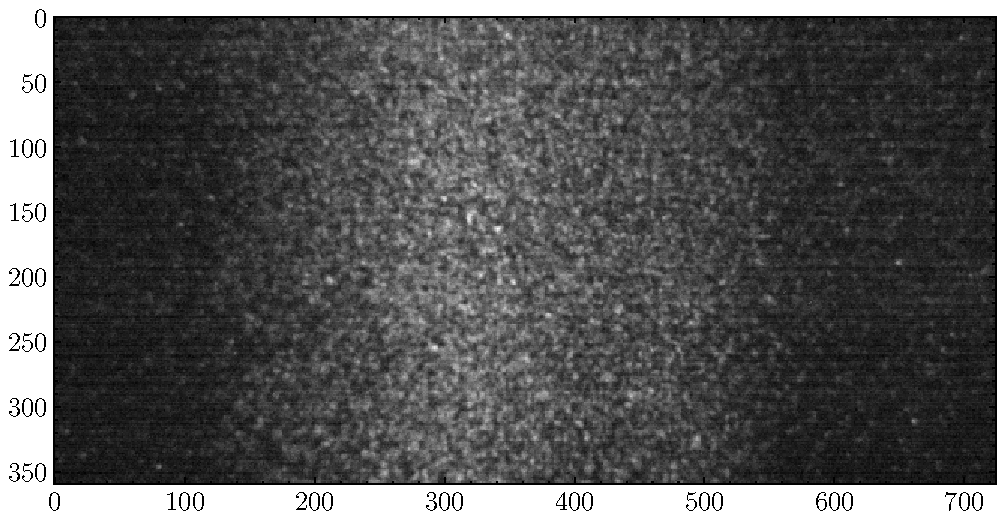
\includegraphics[width=\textwidth]{04_IPHI_Test/figures/fig000_limits_IPHI_a}
    \caption{Beam image}
    \label{chap4:limits_IPHI_a}
  \end{subfigure}

  \begin{subfigure}[t]{1\textwidth}
    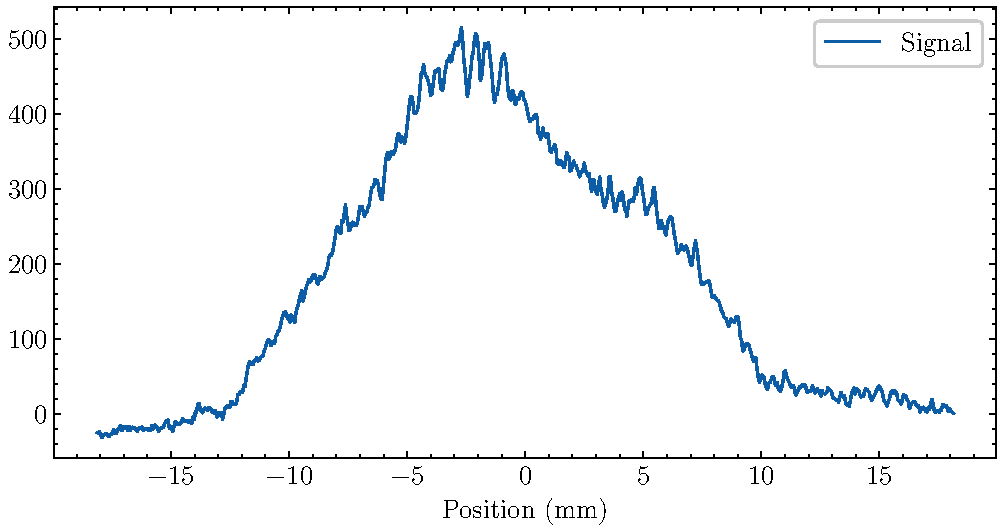
\includegraphics[width=\textwidth]{04_IPHI_Test/figures/fig000_limits_IPHI_b}
    \caption{Projection}
    \label{chap4:limits_IPHI_b}
  \end{subfigure}
  \caption[Example of profile measurement at very low duty cycle.]{Example of profile measurement at very low duty cycle: $0.7\,\mathrm{mA}$, $50\, \mathrm{\mu s}$ and $4 \cdot 10^{-8}\,\mathrm{mbar}$.}
  \label{chap4:limits_IPHI}
\end{figure}


  \FloatBarrier
  \subsection{Electron measurement with MCP}
  Unfortunately, we were not able to measure any profile in electron mode during the first and the second campaign.
  Typical pictures in the electron configuration are shown in Figure \ref{chap4:electron_MCP}. One can see that the profiles cannot be measured correctly since a higher signal is observed on the sides of the \acrshort{mcp}s. During the two test campaigns, comparable patterns were observed on the images in electron mode. The positions of these patterns is not related to the beam position and different beam tuning were performed without any impact on the images.
  The \acrshort{mcp}s are in general a little less sensitive to electrons compared to ions at energies between $5$ and $10\,\mathrm{keV}$ \cite{Wiza1979}.
  However, during tests the signals on the camera were always much higher for electrons than for ions, without any modifications of the gain or the beam conditions. Hence, we suppose that the electron background is huge at \acrshort{iphi}.
  Moreover, electrons are very sensitive to magnetic field; devices like cold-cathode gauges and ion pumps often rely on permanent magnets. During tests, one cold-cathode gauges was installed on the upstream part of the test bench preventing correct profile measurements.
  
  \begin{figure}[!ht]
	\begin{subfigure}[t]{0.5\textwidth}
		\includesvg[width=\textwidth]{04_IPHI_Test/figures/fig000_electron_Hamamatsu.svg}
		\caption{Profile measurement attempt with electrons, Hamamatsu MCP.}
		\label{}
	\end{subfigure}
	~
	\begin{subfigure}[t]{0.5\textwidth}
		\includesvg[width=\textwidth]{04_IPHI_Test/figures/fig000_electron_Photonis.svg}
		\caption{Profile measurement attempt with electrons, Photonis MCP.}
		\label{}
	\end{subfigure}
	\caption[Example of images in electron mode]{Example of images in electron mode for both MCPs.
  Some patterns seem to be the same in the edges and middle of the images.
  The line in the middle is not correlated with the beam.}
	\label{chap4:electron_MCP}
\end{figure}


  \section{Summary}
  \label{ch4:Summary}
  This chapter presented all the developments and tests that have been implemented to address the issues raised in Chapter 3, mainly concerning the choice of the most appropriate readout among three readout technologies. The objective was to experimentally prove the proper functioning of the \acrshort{ipm} method under conditions close to those of \acrshort{ess}.

  First, the feasibility of silicon detectors was verified at the IRMA ion implanter. The results show that detection is possible with dihydrogen ions of $15\,\mathrm{keV}$. However, as soon as the energy is lower or the ions are heavier, the detection is compromised. That is why we have not chosen to continue in this direction.

  The design of the prototypes and the test bench focused on the two remaining methods: strips and \acrshort{mcp}s. The \acrshort{ipm}s and the test bench have been designed to be very versatile, allowing multiple configurations to be tested. Particular attention was paid to system control and vacuum monitoring. The test bench was installed at \acrshort{iphi}, a $3\,\mathrm{MeV}$ proton accelerator, and two test campaigns were carried out.

  The relevant conclusion from the tests shows that the use of a \acrshort{mcp} is mandatory to detect signal at \acrshort{ess} conditions. Hence, the optical \acrshort{ipm} is the preferred solution since it provides higher sensitivity with respect to the strips alone. A relative check of the electrical field uniformity has been performed on both asymmetric and symmetric configurations and with an optical \acrshort{ipm}. The results from the tests show a good agreement with COMSOL simulations.
  Unfortunately, the reference measurements were not exploitable in the experimental conditions, but a good agreement between \acrshort{bpm}s and \acrshort{ipm}s gives more confidence on the measurements.

  We validated our detectors and simulation models as much as experimental condition permitted, in spite of the instability of the machine and the unknown beam conditions. A complete characterization of the prototypes has been achieved.

  From the lessons learned with the prototype, a final design of the cNPM is delivered, including few modifications from the prototype. This will be presented in the concluding chapter.

  \cleardoublepage
  \section{Bibliography}
  \label{ch4:bib}
  \printbibliography[heading=subbibliography]

\end{refsection}

	\chapter{Conclusion and outlook}
\chaptermark{Conclusion and outlook}
\cleardoublepage

\minitoc
%\section{Introduction}
\section*{The cold NPM project for ESS}
\addcontentsline{toc}{section}{The cold NPM project for ESS}
Intense neutron sources are very difficult to achieve. Historically, nuclear reactors have been widely used as intense neutron sources. In Europe the situation is quite critical because most of research reactors will close within the next decade. In this context, the European Spallation Source is being built close to Lund, in Sweden. ESS will push back the limits of existing spallation sources by means of a high and powerful linear accelerator. To ensure the safety of the machine during the commissioning and operations, many diagnostics are foreseen along the accelerator.

This thesis describes the design of one of these diagnostics: the Ionization Profile Monitor (IPM). IPMs are based on the ionization of the residual gas. This is one of the most effective methods, but it is nevertheless quite complex to implement since an IPM operates in vacuum. The first IPMs dated back to the 1960s but the method has been improved significantly with progress in detector, electronics and computer science. The IPM is now mature and used in several installations. In this thesis, the existing methods have been reviewed in order to find the best solution that may match with the ESS requirements. This was first achieved by simulations and, in a second phase, by building and testing prototypes.

\subsection*{Preliminary design review}
\addcontentsline{toc}{subsection}{Preliminary design review}

I started my PhD thesis on October 1$\mathrm{^{st}}$ 2016, 5 months after the kick-off meeting and 4 months before the Preliminary Design Review (PDR). The NPM project for the cold accelerator part was identified as a difficult task with no guaranty about the feasibility of such a monitor, therefore a GoNoGo gate was set for the PDR. In other words, green light to begin the PDR activities would only be given if preliminary studies would receive positive signs to the following challenges:
\begin{itemize}
  \item Very low counting rates: there are low due to firstly the weak residual gas pressure ($10^{-9}\,\mathrm{mbar}$) and secondly due to the low ionization cross-sections that decrease at high energy ($90\,\mathrm{MeV}$ to $2\,\mathrm{GeV}$). Both negative effects have to be compensated by high sensitivity and low noise readouts. Once identified, they have to be assessed to cope with these conditions.
  \item Electric field uniformity: its uniformity must be particularly good to avoid "mirage effects", i.e. forcing the ionization by-products to drift in the parallel direction of the electric field. To achieve such a goal, spaces between IPMs are required. Unfortunately, the vacuum chamber geometry was already frozen (in May 2016, just after the Kick-Off) with small spaces, which would not ease the work.
  \item Space Charge (SC): one of the ESS requirements is to measure the profile with a $10\,\%$ width accuracy. The large SC of ESS is due to the electric field of the proton beam which generates a huge electric field proportional to its energy and its intensity. The low energy ionization by-products are particularly sensitive to this electric field. They are deviated resulting in an enlargement of the measured beam profile. This effect could not be estimated by simple calculations and sophisticated simulations were developed to solve this issue.
\end{itemize}

My first urgent tasks when I joined the NPM team at Saclay were to estimate counting rates and to participate to the readout choice to check compliance to the requested low sensitivity. The PDR took place at ESS Lund on January 31$\mathrm{^{st}}$ 2017, where we presented our preliminary results giving confidence on the IPM feasibility. The GoNoGo gate was passed successfully, opening to the next phase of the project. In this phase, we needed to demonstrate through prototype design, beam tests and calculations that IPM fulfilled the ESS requirements. We also needed to provide a final solution for the manufacturing of the IPMs.

\subsection*{Prototypes and test bench development}
\addcontentsline{toc}{subsection}{Prototypes and test bench development}

An IPM must be self-consistent on its support, here a flange CF200. This imposes to have all the HV connectors, the grounding, the readout system attached on it meaning that once the IPM is integrated, it can be inserted into the test bench vacuum CF200 aperture, like a drawer. Originally, 3 readout types were considered. The Timepix option had to be discarded due to incompatibility with ion detection. Finally two readouts were selected: a conductive strips plane and a MCP read by a CMOS camera. Two reference systems were also installed, one based on fluorescence and an interceptive screen with 3 solid scintillators. The bench was made of two parts; the first had similar dimensions of the ESS LWU, with 2 IPM locations and another one, on the second part.
The strips IPM could be polarized in asymmetric mode, whilst MCP IPM could be operated on both modes. All along the integration, we encountered many vacuum problems, which were solved by baking. We currently reached $2$-$3 \cdot 10^{-7}\,\mathrm{mbar}$.
We also faced sparks when reaching $30\,\mathrm{kV}$ with high voltage connectors weakly insulated and connection boxes. In parallel, I greatly improved the uniformity of the IPM electric field by tuning the resistor bridge, but also by inserting a disk in the vacuum chamber, with a circular aperture as large as the beam pipe. This is mandatory to avoid the cross-interaction between both IPM electric field tilted at $90\mathrm{^{o}}$ with respect to each other.
I also implemented the software for several applications control systems (HV, pressure probes...) using the EPICS framework.

\subsection*{Beam tests at IPHI}
\addcontentsline{toc}{subsection}{Beam tests at IPHI}

We installed the test bench on mid-2017 at IPHI. The first beam was delivered and there was no diagnostic working on IPHI, only an ACCT located upstream of our bench and a Faraday cup working as beam dump. Moreover the commissioning of IPHI was not done for the higher energy part (downstream the RFQ, at $3\,\mathrm{MeV}$). Before to obtaining a beam profile, we needed two weeks of tuning with a beam dynamic physicist in order to adjust the deviation dipole, the correction steerers and the quadruples. However the beam presented a strange behavior showing a position oscillation. Charging effects on our detectors were suspected by all the experts. A couple days later, the BPM finally observed the same position oscillations confirming our measurements. IPHI has not yet an explanation of this effect. Our IPMs had an important role in the characterization of this effect.

We also discovered that the beam presents 2 components: a mix of a core and narrow beam at high beam intensity and a larger component at low intensity. Another concern was to make systematic studies due to difficulties on the reproducibility of the beam. Nevertheless, it was useful to have such versatile facility where we were able to regain the expected MCP behavior. Many measurements were done, allowing investigating many parameters and preparing the second beam tests in September 2018.

The goal of the second test was to focus on the profile measurement feasibility in nominal ESS conditions, in ion mode since simulations already shown that electron detection could not be used for profile purposes. During this last campaign, we finally worked in such beam conditions, and even worse than the ESS ones. These results are summarized in the Table \ref{chap4:extrapolationMCP} demonstrating the feasibility of the measurement of the beam profile for each pulse beam with ESS nominal conditions.

\section*{Ongoing work}
\addcontentsline{toc}{section}{Ongoing work}

The following sections present current actions for the design of the final detectors as well as the more distant perspectives.
%The type of these tasks is quite broad, so it is interesting to describe them briefly.
%
\subsection*{Background signal estimation}
\addcontentsline{toc}{subsection}{Background signal estimation}

During the project reviews we were asked to study the influence of background noise on the IPM readouts. This is a complex task because it requires enough background particle information  and a realistic geometry.

A Geant4 simulation has been prepared in order to answer this request. The simulation includes a mixed geometry including shapes made from primitive geometry (LWU, support, MCP) and complex elements imported from CAD files (IPM, camera, magnet). Fig. \ref{chap5:fig:Geant4} shows the implemented geometry of the LWU with the two IPMs, the quadrupoles and the cameras with their sensors. The choice of the physics list can be quickly modified using the predefined lists in Geant4. The elements to be studied use the Sensitive Detector mechanism enabling to save information about the particles passing through them. As the data flow is important, the simulation results are saved using the ROOT interface provided in Geant4. The simulation uses the new multithreading features of latest versions of Geant4 and an OpenMPI layer has been added \cite{Allison2006,Dotti2016}. The simulation code is completely ready and the background particle information that was only made available very recently needs only to be included to launch the simulations.

I hope that this work will continue and lead to results that may provide additional knowledge.

\begin{figure}[!ht]
	\begin{subfigure}[t]{0.385\textwidth}
		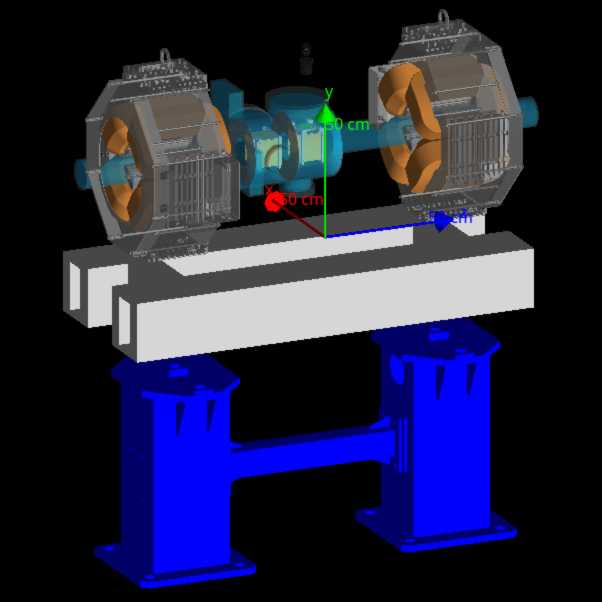
\includegraphics[width=\textwidth]{05_Conclusion/figures/fig000_geant4_sim2_a}
		\caption{The LWU and two quadrupoles.}
		\label{}
	\end{subfigure}
	~
	\begin{subfigure}[t]{0.615\textwidth}
		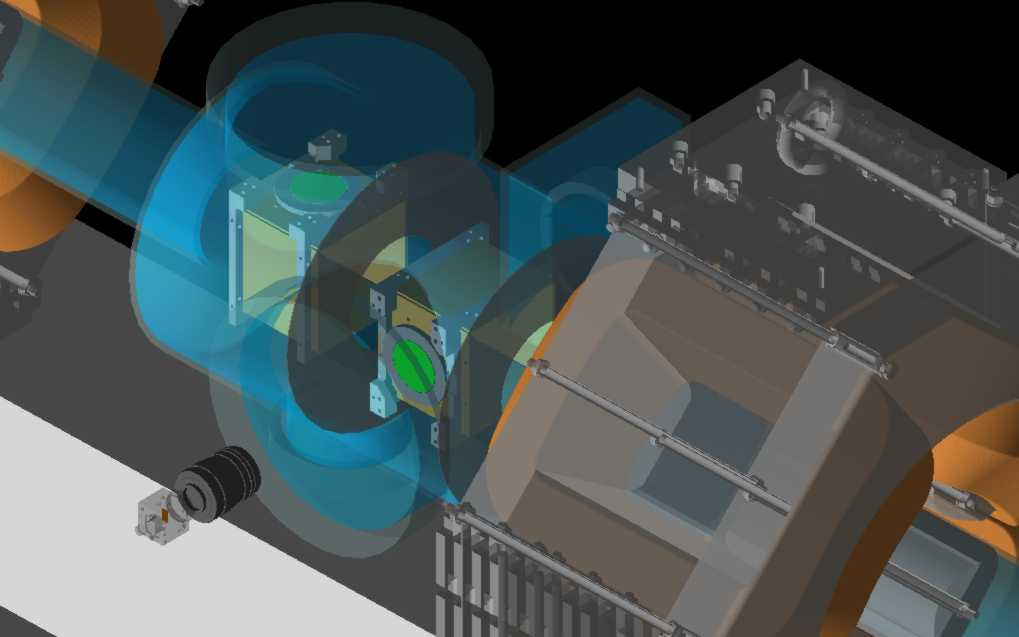
\includegraphics[width=\textwidth]{05_Conclusion/figures/fig000_geant4_sim2_b}
		\caption{Zoom on the two IPMs.}
		\label{}
	\end{subfigure}
	\caption[The geometry implemented in Geant4]{The geometry implemented in Geant4.}
	\label{chap5:fig:Geant4}
\end{figure}



% Florian: Je ne sais pas si il y a une échéance ? La production a plus ou moins déjà commencé
% All these aspects should be finalized by xxx (une date) allowing the production, installation and commissioning of the IPMS at ESS in xxx (autre date).

\subsection*{MCP calibration}
\addcontentsline{toc}{subsection}{MCP calibration}

\begin{wrapfigure}{l}{0.5\textwidth}
  \includegraphics[width=0.5\textwidth]{example-image-a}
	\caption[The calibration of the MCP is done with a VUV lamp]{The calibration of the MCP is done with a VUV lamp.}
	\label{chap5:fig:UV_calib}
\end{wrapfigure}

MCPs are mandatory to measure a profile with IPM in the ESS conditions. Unfortunately, these devices are sensitive to ageing effects. The gain will decrease over  time in the impacted areas by ions. Since the ESS beam will be stable in position, the MCP region in front of the beam will be more affected.

Therefore, at some point the profile measurement will be no longer reliable. To overcome this phenomenon it is necessary to calibrate the MCP regularly, i.e. perform a gain mapping and correct the profile by a software adjustment. This requires an uniform and stable source that routinely irradiates the MCP. The most common method relies on a VUV source \cite{Giacomini2011}. MCPs become sensitive to the photoelectric effect for wavelengths shorter than $200\,\mathrm{nm}$. The most basic VUV sources are deuterium discharge lamps that have broadband emission with a peaks at $160\,\mathrm{nm}$ \cite{HamamatsuUV,NewportUV}. It is also possible to generate VUV with excimer lasers or by using high order harmonic generation. Thermoionic emission was discarded due to the requirements imposed by the superconducting cavities. We are also considering the use of Electron Generator Arrays \cite{Satou2006, PhotonisEGA}. The calibration is currently being tested on the IPM test bench and Fig. \ref{chap5:fig:UV_calib} shows the principle of the experiment.

\subsection*{Remote acquisition system}
\addcontentsline{toc}{subsection}{Remote acquisition system}

In the case where the radiation background should shorten the MCP lifetime down to a year, it would be necessary to set a camera at remote distance in a shielded area. Two solutions are investigated to transport the image over up to $10\,\mathrm{m}$, where the camera can be shielded in the bottom of the nearby Stub. The solution to get a camera detecting single events, i.e. an ion hitting the MCP is been studied at ESS. The document presents two alternative imaging systems: the first one using a fiberscope and lenses is sketched on Fig. \ref{chap5:fig:schematic:1}, while the other one based on 2 mirrors and an objective lens can be seen on Fig. \ref{chap5:fig:schematic:2}.

\begin{figure}[!ht]
	\begin{subfigure}[t]{0.5\textwidth}
		\includegraphics[width=\textwidth]{05_Conclusion/figures/fig000_schematic_telescop_lens}
		\caption{}
		\label{}
	\end{subfigure}
	~
	\begin{subfigure}[t]{0.5\textwidth}
		\includegraphics[width=\textwidth]{05_Conclusion/figures/fig000_schematic_coherentr_fiber}
		\caption{}
		\label{}
	\end{subfigure}
	\caption[]{}
	\label{chap5:schematic}
\end{figure}


Using a first order evaluation of the system transmission, one can start by selecting the focal lens required to make conjugate images. For the lens L1, the magnifications for the MCP is set, so as the geometrical aperture coupling light into the fibre.

The geometrical transmission for 0.5 numerical aperture of the fiberscope is about $3 \cdot 10^{-5}$ while it is a factor 4 below for the second system. Such an attenuation encourages to purchase stacked double MCP for increasing the output light.

The fiber attenuation is an important property to take into account. For instance, for silica fibers, this can be as low as a few $\mathrm{dB/km}$. We intent to use plastic coherent fibers. The material used is PMMA. This material is rather cheap, and it presents good optical quality and rather good transmission, typically $0.5\,\mathrm{dB/m}$ at $500\,\mathrm{nm}$. However, a full characterization of the system with the selected fiber will have to be done in order to prove and demonstrate the performance of the system. Lenses transmissions can be close to $100\,\mathrm{\%}$ with anti-reflection coating.

\subsection*{Final IPM design and production}
\addcontentsline{toc}{subsection}{Final IPM design and production}


% TODO: Finir
From the lessons learned with the prototypes, a final design of the IPM is on going\footnote{The design of final IPM has started, but is not frozen yet}, including few modifications from the prototype. This section presents briefly the new IPM design and its characteristics as well as the IPM production strategy. The differences between the prototypes and final IPMs are reported in Table \ref{chap5:tab:recap}. 

Preliminary simulations exhibit that the detection is possible if the readout system is enough sensitive. An important concern was about the choice of this readout. However without full characteristics of each system it is almost impossible to simulate the limits of detections. Therefore, these limits has been determined directly during beam tests. The tests clearly underline that the use of MCP is the best solution. Single stages MCP have been used during tests and they seems sufficient to detect profile at ESS. However IPMs will probably be ready before the accelerator reaches nominal conditions and double stage MCPs will allow profile measurements during the accelerator commissioning. The use of a double stage MCP reduces the maximal resolution achievable but this reduction is less important than the one induced by the remote acquisition system. The MCP with a strips readout provides the best performances in term of sensitivity and speed but needs a specifically designed readout electronics. Whereas an optical  MCP exposes decent performances with a high resolution and the acquisition relies only on \acrshort{cots} cameras. At the end the optical solution has been chosen. In any case the design of IPMs allows to easily upgrade the readout for future improvements thanks to the new mechanical design presented below.

Two field configurations were considered for the extraction field: asymmetric and symmetric. Simulations show that the symmetric setup provides a very good electric field uniformity even in longitudinal direction with simpler corrections. But asymmetric configuration also meets the requirements, and both case can be forseen at ESS since MCPs will be used. The electric field simulations have been verified with a relative comparison between the two cases and a good agreement has been observed. In practice, the symmetric configuration reduces the maximum potential to apply on each electrode reducing the need of HV feedtroughts above $20\,\mathrm{kV}$. These feedtroughs are complex, big and fragile increasing the complexity of the design. On the other hand, the number of HV power supplies, required in symmetric, mode is higher. Therefore the design is more expensive. For the final IPM, a $\pm\,15\,\mathrm{kV}$ symmetric configuration is forseen.

Space charge simulations point out that the measurement should be performed with ions at ESS. The in-house model has been checked during beam tests with the IPHI parameters. According to simulations, an electric field value of $2$ to $3\,\mathrm{kV/cm}$ seems enough and the final IPM design will target these electric field ranges. However it was not possible to reach stricly the same ESS bunch configuration. During the beam tests, the prototypes were not able to measure in electron mode whereas prototypes in ion mode were working fine. This strengthens the choice of ions for the profile measurement.

\begin{table}[!h]
  \centering
  \caption[Summary of differences between the prototype design and the final design]{Summary of differences between the prototype design and the final design.}
  \label{chap5:tab:recap}
  \begin{tabularx}{\linewidth}{lXX}
    \toprule
              & Prototype                                    & Final design            \\
    \midrule
    Amplifier & Single stage MCP                             & Double stage MCP        \\
    Readout   & Strips or phosphorus screens                 & Phosphorus screen (P43) \\
    Polarity  & Symmetric or asymmetric                      & Symmetric               \\
    Particle  & Ions or $e^{-}$                              & Ions                    \\
    Voltage   & $\pm 10\,\mathrm{kV}$ or $0/30\,\mathrm{kV}$ & $\pm 15\,\mathrm{kV}$   \\
    \bottomrule
  \end{tabularx}
\end{table}

The final IPMs will be produced following the ESS requirements for the superconducting cavities meaning that the IPMs will be assembled within an ISO-5 clean room environment.

During the tests at IPHI, we used a simple CF200 flange to support the IPM (Fig. \ref{chap4:IPM_photo2}). For the manufacturing of the IPM, we thought that two independent flanges CF200 and CF160 (Fig. \ref{chap5:fig:bride_double}) will ease the assembling process and the maintenance in clean room environment. This later configuration presents different advantages.

\begin{figure}[!ht]
	\begin{subfigure}[t]{0.25\textwidth}
		\includegraphics[width=\textwidth]{05_Conclusion/figures/fig000_bride_double2_a}
		\caption{A 3D drawing of the new design.}
		\label{}
	\end{subfigure}
	~
	\begin{subfigure}[t]{0.75\textwidth}
		\includegraphics[width=\textwidth]{05_Conclusion/figures/fig000_bride_double2_b}
		\caption{The new design allow to remove MCP easily and is independent to the IPM direction.}
		\label{}
	\end{subfigure}
	\caption[The new IPM design]{The new IPM design \cite{JacquesCDR2019}.}
	\label{chap5:fig:bride_double}
\end{figure}

Once the complete IPM set is mounted on the LWU, alignment can be done by measuring all sight pods on the CF200. Then, if the MCP has to be removed (unscrew the CF160), the IPM cage linked to the CF200 stays fixed. The MCP can be changed but no alignment is necessary. This new configuration is compliant with a better reliability of the IPM since the MCP change may be done quickly, with no impact on alignment. The IPMs X and Y are similar: while X is centered on the CF200 LWU viewport, Y is shifted by $36\,\mathrm{mm}$ to its CF200 axis. The trick for mounting both IPMs, is to rotate the CF160 by $180°$ with respect to the CF200 flange. This is of great interest for manufacturing purposes.

For assembling the whole IPM, it is more convenient to prepare first the CF200 and all its belonging items, and then the CF160 ones. It allows minimizing the MCP in oxygen atmosphere. Furthermore, the set made of CF160 and MCP holder is light with a small lever arm easy to manipulate.

The IPMs will be delivered by pair and the first pairs are expected to be delivered to ESS at the middle of 2020.

Let's finish this manuscript from a perspective that goes beyond the ESS project. IPHI is a unique machine due to its powerful injector, but it has suffered delays in the past due to unfortunate circumstances. Over the last three years, a new dynamic is underway to fully exploit the accelerator capabilities. Today, IPHI is the first step of a new national compact neutron source: SONATE \cite{Marchix_2018}. As stated in the first chapter, the LLB is closing its last research reactors this year. Some estimates show that the availability of neutrons at the national level will fall by more than $90\,\mathrm{\%}$ within the next 10 years.

During the tests, the versatility of IPHI greatly helped to characterize the IPMs. However, some tests were limited by a lack of beam information during operation. Indeed, only two types of diagnosis were available: BPMs and BCMs. IPMs are a very interesting solution for IPHI because they measure the size and  the position in a non-intrusive way. A close collaboration has started in order to provide to IPHI an IPM system that fulfills the present and future needs. This new project will greatly benefit from the studies and experiences presented in this thesis.

\cleardoublepage
\section*{Bibliography}
\addcontentsline{toc}{section}{Bibliography}
\label{ch2:bib}
\printbibliography[heading=subbibliography]

%%%%% 
%Firstly, we discovered that one of the pMCP was broken and finally decided to change it.

%After more than 2 weeks, we did not have seen a beam profile. We finally succeeded after working thoroughly with a beam dynamic physicist, scanning the beam as well as the deviation dipole, the correction steerers and the quadruples. We effectively got a nice transverse profile, completely correlated to the beam location and intensity, but having a strange behavior. Indeed, the pulse presented a position oscillation, starting to move in one direction, and coming back after $5$-$7$ seconds to its initial position, and so on! It was similar to an insulator, starting to accumulate electric charges and releasing them suddenly… We inquired on our IPM which are designed with insulators (Peeks, Macor, ceramics), since we did not find anything strange on the beam side. It lasted several days with any explanation, until a physicist gets to work on a BPM, to discover a very impressive correlation between the BPM and the IPM beam coordinates! Up to now, IPHI has not a real explanation for this behavior. This event sounds like a big relief and gave us a better confidence in our measurements.

%  Later on, we discovered that the beam presents also 2 components as shown in the manuscript: a mix of a core and narrow beam at high beam intensity and a large component at low intensity.
%  We have also encountered some difficulties to make systematic studies because it is not easy to reproduce a beam condition, even with previously beam parameters. Nevertheless, it was useful to have such versatile facility where we were able to regain the expected MCP behaviors. Many measurements were done as shown in the thesis, allowing investigating many parameters and for preparing the second beam tests on September 2018. The goal will be to focus on the profile measurement feasibility in nominal conditions, in ion mode since simulations have already shown that electron detection is hopeless.

%  During this last campaign, we finally work in such beam conditions, which are even worse than the ESS ones. These relevant results are summarized in the Table \ref{chap4:extrapolationMCP} demonstrating that we should be able to measure beam profile at ESS at nominal conditions, for each pulse beam.

%%
% In this manuscript I presented a large part of the work done on the study, design and testing of non-invasive profilers based on ionization. This chapter describes the tasks currently underway or in perspective for the conception of the final diagnostics and summarize the previous chapters. 

% The MCP is 40\,mm diameter and the fiber diameter is 2\,mm. The geometrical transmission T of the lens to the fiber is defined by the aperture of the lens, called the F-number or F\#, the focal lens, F and the distance between the screen and the lens, D1:
% \begin{equation}
%  T=\frac{1}{2} \left(1 - cos\left(\theta\right)\right)
% \end{equation}
% with $\theta = \rm arctan\left (\frac{F/F\#}{2D} \right )$

% Unfortunately, the information about the background particles was finally given after the beginning of the writing phase of this thesis. Nevertheless, the simulation base is implemented and I hope that this work will continue and lead to results that may provide additional knowledge.
% \section*{Conclusion}
% \addcontentsline{toc}{section}{Conclusion}

% \subsection*{The ESS linac and IPM}
% \addcontentsline{toc}{subsection}{The ESS linac and IPM}

% Intense neutron sources are very difficult to achieve. Historically, nuclear reactors have been widely used as intense neutron sources. In Europe the situation is quite critical because most of research reactors will close within the next decade. In that context, the European Spallation Source is being built close to Lund, in Sweden. ESS will push back the limits of existing spallation sources by means of an high end powerful linear accelerator. To ensure the safety of the machine during the commissioning and operations, many diagnostics are foreseen along the accelerator.

% This thesis described the design of one of these diagnostics: the Ionization Profile Monitor(IPM). IPMs are based on the ionization of residual gas. This is one of the most effective methods, but it is nevertheless quite complex to implement. The first IPMs date back to the 1960s but the method has been improved significantly with advances in detector, electronics and computer sciences. The IPM method is now mature and used in several installations. In this thesis, the existing methods have been reviewed in order to find the best solution that may match with the ESS requirement. This have been done by simulations first and, in a second time, by building and testing prototypes.

% \subsection*{IPM feasibility}
% \addcontentsline{toc}{subsection}{IPM feasibility}

% Three key points had been identified: number of primary particles, distortion effects of the profile, the choice of the reading system.

% The conditions at ESS are particularly unfavorable for the ionization cross sections and the high vacuum in the accelerator does not work in our favour. Calculations (Bethe and PAI) and simulations show that the order of magnitude of the number of primary particles is about a few thousand particles per pulse beam under nominal ESS conditions. This number seems sufficient to carry out a measurement assuming that tey are correctly detected.

% Non-uniformities of the electric field can be effectively corrected using field correctors and separation discs regardless of the power supply configuration used. However, the symmetrical mode is easier to correct and reduces the maximum voltage level required.
% Simulations clearly show that ions are less sensitive to the space charge effect and initial velocity of particle. Measurement with electrons introduces an error that does not allow the ESS requirements to be met. It is impossible to install a corrector magnet to constrain the electron trajectories. Therefore, the profile measurement will be done with ions.

% The use of ions makes the choice of the readout a more complicated. Strips are an robust method but require enough sensitive and low-noise electronics to be able to detect such low charge quantities.
% The MCPs amplifies the signal but these devices tend to age. Silicon detectors look very promising because they are very sensitive, resistant and fast. However, the detection of low energetic ions is not ensured and the implementation is quite complex.

% \subsection*{Prototype design and tests}
% \addcontentsline{toc}{subsection}{Prototype design and tests}

% First, the feasibility of silicon detectors was verified on the
% At IRMA ion implanter, the feasibility of silicon detectors was checked.
% The detection seams possible but with almost no error margin. We also observed that the silicon sensor was quickly damaged by the incident ions. Therefore, we discarded this readout for ESS usage.

% Then, a complete IPM testing platform has been developed in order to test the two remaining readouts. The IPM prototypes have been designed to be totally independent to the readout. Therefore the testing platform was quite versatile.

% The prototype been tested at IPHI, a $3\,\mathrm{MeV}$ proton accelerator. A complete characterization of the two IPMs was done. Good agreements have been found between the two types of IPMs and existing IPHI diagnostic. The tests were also a kind a commissioning of the machine confirming that the IPMs is a great tool to tune a beam. According to results the measurement seams possible at ESS with even a single stage MCP. The results has been presented to ESS collaborators during a Critical Design Review.

% The final IPM will use double stages MCP polarized in symmetric HV configuration. The symmetric setup provides really good uniformity with basic corrections. It also reduces the maximum potential to apply to electrode.
% A MCP with strips may provides best performances in term of sensitivity and speed. But a complicated readout electronic must be designed for that purpose. Whereas a MCP optical exposes decent performances and an high resolution but the acquisition relies only on COTS cameras.
% At the end the optical solution was chosen. Anyway the design of IPMs allows to easily upgrade the readout for future improvements.

% The double stage MCP will allow measurement during the accelerator commissioning. Therefore may be ready even before than the accelerator reaches its nominal conditions. On the other hand the use of an double stage MCP reduces the maximal resolution but this reduction is less important compare to the one induced by the remote acquisition system

% The final IPMs will be produced following the ESS requirement for the superconducting cavities. This means that the IPMs will be assembled within an ISO-5 clean room environnement. The IPMs will be delivered by pair and the first pairs is expected to be delivered to ESS in the beginning of 2020.

%\subsection{Personal conclusion}

%\end{refsection}


	\printglossary[type=\acronymtype]

	\listoffigures
	\addcontentsline{toc}{chapter}{\listfigurename}

	\listoftables
	\addcontentsline{toc}{chapter}{\listtablename}
\end{otherlanguage}

\begin{otherlanguage}{french}
	\chapter*{Résumé en Français}
\markboth{Résumé en Français}{}
\addcontentsline{toc}{chapter}{Résumé en Français}%

% Neutron
Le neutron est une particule non élémentaire dépourvu de charge avec une masse proche de celle du proton. Il possède également un spin de $\frac{1}{2}$ et un moment magnétique faible. Le neutron étant une particule neutre, il n'interagit que très peu avec le cortège électronique du milieu contrairement aux particules chargées. Un neutron peut ainsi parcourir de grandes distances sans subir d’interactions majeures. Celles-ci se faisant principalement avec les éléments du noyau par interaction forte. Les neutrons sont devenus des outils très intéressants pour de nombreux domaines de la science. Ces particules permettent de sonder la matière à différent niveau d'échelle et de temps via des méthodes variées. Les applications dépassent largement la physique et peuvent concerner des domaines variés comme la biologie, les sciences des matériaux et même l'archéologie.

% Sources neutrons
Cependant il est beaucoup plus compliqué de produire des neutrons que des particules chargées ou même des photons. L'une des méthodes de production de neutrons consiste à utiliser des sources composites type alpha-béryllium. Cependant ces sources sont limitées à des faibles flux de neutrons. Les infrastructures de recherches actuelles reposent plutôt sur des réacteurs à fission produisant un flux intense et continu de neutrons.
Le fonctionnement de ce type d’installation nécessite une gestion de la sécurité et des matières radioactives. Les réacteurs de recherche souffrent également de l’image du nucléaire ce qui peut freiner l’investissement dans ce type d’installation.

Depuis quelques années, les sources de neutrons pilotées par accélérateur sont devenues des alternatives crédibles face aux réacteurs et de nombreux projets de source à spallation ont vu le jour. Cela est rendu possible grâce aux progrès réalisés dans les technologies des accélérateurs de particules. Les sources se basant sur la spallation sont les plus efficaces mais aussi les plus complexes à mettre en oeuvre. Le fonctionnement de ce type de source est le suivant : des protons de hautes énergies (de la centaine de MeV au GeV) vont entrer en collision avec une cible dense. Les noyaux de la cible vont se désintégrer sous la violence du choc et des neutrons sont libérés sur un large spectre en énergie. Les neutrons sont ensuite thermalisés et transportés vers différentes expériences. Les première sources à spallation ont vu le jour dans les années 70-80, puis une seconde génération a été developpée dans les années 2000. L'évolution des différentes sources de neutrons est montrée dans la Figure \ref{sumfr:fig:NeutronSources_a}.
\begin{figure}[!ht]
	\begin{subfigure}[t]{0.5\textwidth}
		\includegraphics[width=\textwidth]{00_French/figures/fig000_NeutronSources_a}
		\caption[]{Evolution des sources de neutrons thermiques depuis la découverte du neutron.}
		\label{sumfr:fig:NeutronSources_a}
	\end{subfigure}
	~
	\begin{subfigure}[t]{0.5\textwidth}
		\includegraphics[width=\textwidth]{00_French/figures/fig000_NeutronSources_b}
		\caption[]{Prévision du temps instruments pour chaque source de neutrons Européennes.}
		\label{sumfr:fig:NeutronSources_b}
	\end{subfigure}
	\caption[]{Historique des sources de neutrons et prospectives Européennes  d'après un rapport de l'ESFRI datant de 2019.}
	\label{sumfr:fig:NeutronSources}
\end{figure}


Actuellement, les réacteurs de recherche constituent les principales sources de neutrons en Europe. Cependant ces installations sont pour la plupart vieillissantes et aucune stratégie claire de renouvellement n'a été mise en oeuvre durant les dernières décennies. Ces installations doivent fermer d'ici une dizaine d'années et l'accès aux sources de neutrons risque de devenir critique pour la  communauté scientifique Européenne, comme le montre la Figure \ref{sumfr:fig:NeutronSources_b}. Pour conserver les compétences et les savoirs dans ces domaines, la communauté Européenne a impulsé un mouvement de renouveau se basant en partie sur la création d'une source de neutrons ultra intense nouvelle génération.

% ESS
La Source de Spallation Européenne (ESS) sera la future source de neutrons, elle est actuellement en construction à Lund en Suède. L’objectif de ESS est de devenir la source pulsée de neutrons la plus brillante au monde. La Figure \ref{sumfr:fig:ESS_pulse} montre les différences en terme de brillance entre ESS et les sources existantes. Les premiers neutrons sont attendus pour 2022 afin de prévenir la fermeture des principaux réacteurs  d’ici les prochaines années. Lors du démarrage du faisceau, 15 instruments de spectroscopie, de réflectométrie et de diffraction neutronique seront disponibles pour les chercheurs et les partenaires industriels dans des domaines variés. Puis dans une phase d’extension, 7 nouveaux instruments seront installés à ESS.
\begin{figure}[!ht]
  \begin{center}
    \includegraphics[width=0.85\textwidth]{00_French/figures/fig000_ESS_pulse}
  \end{center}
  \caption[]{Comparaison de la brillance d'ESS par rapport aux différentes sources de neutrons existantes.}
  \label{sumfr:fig:ESS_pulse}
\end{figure}


ESS peut être résumée grossièrement en 3 parties : un puissant accélérateur linéaire (linac), une imposante cible en tungstène et une dizaine d’instruments à neutrons. Chacun de ces éléments représente une rupture technologique dans leur domaine respectif. La spécificité de ESS est son accélérateur linéaire pulsé de haute intensité qui sera l’un des plus puissant au monde. Pour se faire, le linac de ESS se base massivement sur des cavités supraconductrices qui permettent d'accélérer des impulsions longues et intenses dans des dimensions raisonnables. Le coût total de construction est estimé à $1$ milliard € et le coût de fonctionnement annuel sera d'environ $100$ million €.
\begin{figure}[!ht]
	\begin{center}
		\includegraphics[width=\textwidth]{00_French/figures/fig000_ESS_acc}
	\end{center}
	\caption[]{Représentation simplifiée du linac de ESS. Les blocs bleus représentent la partie supraconductrice de l'accélérateur où les IPM seront installés.}
	\label{sumfr:fig:ESS_acc}
\end{figure}


% IPM
Les diagnostics faisceau servent à s’assurer du bon fonctionnement de l'accélérateur et garantissent la sécurité des personnes et des installation en cas de dysfonctionnement. Ils permettent de mesurer différentes caractéristiques du faisceau comme le courant, la position, l’énergie, l'émittance, les profils et les pertes.. Pour chaque caractéristique du faisceau plusieurs méthodes peuvent être considérées, avec pour chacune des avantages et des inconvénients. Les diagnostics faisceau sont donc à la croisée de nombreux domaines de la physique.

La mesure de profils transverses donne une information sur la répartition du faisceau dans son plan transversal. C'est une donnée très intéressante pour les physiciens de la dynamique faisceau. Ces mesures peuvent être séparées en deux types. Les méthodes intrusives ou invasives qui entrent en interaction directe avec le faisceau allant même jusqu'à le détruire, et les non invasives qui ont des interactions négligeables ou nulles avec le faisceau. Dans la partie supraconductrice de ESS, la mesure du profil dans les conditions nominales doit se faire de manière non invasive. La méthode retenue est basée sur la collection directe des produits d'ionisation du gaz résiduel par un champ électrique. Ce type de moniteurs est appelé Ionization Profile Monitor (IPM). Son principe de fonctionnement est illustré dans la Figure \ref{sumfr:fig:ipm_outline} et peut être synthétisé en trois grandes étapes:
\begin{wrapfigure}{r}{0.5\textwidth}
	\centering
	\begin{tikzpicture}%[scale=1.3]
		% Variables
		% Ipm
		\pgfmathsetmacro{\LIPM}{1.8};
		\pgfmathsetmacro{\HIPM}{1.8};
		\pgfmathsetmacro{\TIPM}{0.1};
		% Deg
		\pgfmathsetmacro{\LDEG}{0.1};
		\pgfmathsetmacro{\HDEG}{0.3};
		\pgfmathsetmacro{\NDEG}{6};
		\pgfmathsetmacro{\SDEG}{1.5};
		\pgfmathsetmacro{\SPAND}{(2*\SDEG - \HDEG)/\NDEG}

		\draw[] (\LIPM,0) node[right,align=left] {Field\\correctors\\or\\degraders};

		% Beam
		\draw[fill=blue!30] (0,0) circle (0.4) node[left,xshift = -0.3cm] {Faisceau};
		% Cage
		\draw (0,0) (-\LIPM,\HIPM)rectangle(\LIPM,\HIPM+\TIPM) node[above] {Anode};
		\draw (0,0) (-\LIPM,-\HIPM)rectangle(\LIPM,-\HIPM-\TIPM) node[below] {Cathode};
		\draw[fill=red!50] (-\LIPM/2,-\HIPM) rectangle(\LIPM/2,-\HIPM-\TIPM) node[midway,below] {Détecteur};
		% Ionized particle
		\draw[blue, dashed,->] (0.1,0.8)--(0.1,\LIPM);
		\draw[blue,fill=blue] (0.1,0.8) circle [radius=1mm] node[] {\tiny\color{white}{$-$}};

		\draw[red, dashed,->] (0.16,-1)--(0.16,-\LIPM);
		\draw[red,fill=red] (0.16,-1) circle [radius=1mm] node[] {\tiny\color{white}{$+$}};

		\draw[blue,dashed,->] (-0.1,0.1)--(-0.1,\LIPM);
		\draw[blue,fill=blue] (-0.1,0.1) circle [radius=1mm] node[] {\tiny\color{white}{$-$}};

		\draw[red,dashed,->] (-0.1,-0.1)--(-0.1,-\LIPM);
		\draw[red,fill=red] (-0.1,-0.1) circle [radius=1mm] node[] {\tiny\color{white}{$+$}};

		%Field
		\draw[->] (-1.2,1.5)--(-1.2,0.6) node [midway,right]{$\vec{E}$};
		% Degradors
		\foreach \x in {0,...,\NDEG}{
				\draw (0,0) (-\LIPM,\x*\SPAND - \SDEG) rectangle (-\LIPM+\LDEG,\x*\SPAND+\HDEG-\SDEG);
				\draw (0,0) (\LIPM,\x*\SPAND - \SDEG) rectangle (\LIPM-\LDEG,\x*\SPAND+ \HDEG-\SDEG);}


		%Profile
		\begin{axis}[every axis plot post/.append style={
						mark=none,domain=-3:3,samples=50,smooth},
				clip=false,
				axis y line=none,
				axis x line*=bottom,
				ymin=0,
				ymax=1,
				xtick=\empty,
				width=4cm,
				height=3cm,
				scale only axis,
				xshift=-2cm,
				yshift=-3.5cm
			]
			\addplot {\gauss{0}{0.3}{0.3}};
		\end{axis}

	\end{tikzpicture}
	\centering
	\caption[]{Représentation synthétique du fonctionnement d'un IPM}
	\label{sumfr:fig:ipm_outline}
\end{wrapfigure}

\begin{enumerate}
  \item Les protons du faisceau passent à travers le gas résiduel dans le tube à vide de d'accélérateur. Cela induit une ionization: des paires électron/ion sont créées.
  \item Dans l'IPM, un fort champ électrique conduit les électrons ou les ions\footnote{Cela dépend de la polarisation de l'IPM.} vers un système de détection segmenté.
  \item Le profil est reconstruit dans une direction transverse. Pour un profil complet, une paire d'IPM, avec un IPM pivoté de $90\textdegree{}$ par rapport à l'autre, est nécessaire.
\end{enumerate}
Les IPM sont assez communs sur les anneaux de stockage de protons/hadrons où les pressions de gaz résiduel sont très basses. L’utilisation de plus en plus fréquente des cavités supraconductrices dans les accélérateurs linéaires fait que cette méthode devient également intéressante pour ce type d'accélérateurs. Cette thèse présente le travail effectué lors du développement d’un IPM pour la partie supraconductrice de l’accélérateur de ESS.

% Simulation
La simulation d’un IPM est décomposée de la même façon que son fonctionnement décrit plus haut. Dans un premier temps il convient de savoir si le nombre de particules initialement créées est suffisant pour être détecté. Cependant cela ne donne pas la certitude de pouvoir mesurer un profil correct. Il faut prendre en compte les différents effets électromagnétiques qui vont influer sur la trajectoire des particules. Ces effets peuvent distordre la projection du profil et faire perdre des particules. La dernière étape consiste à évaluer la réponse de l'élément de détection en fonction des caractéristiques de la particule incident. La nature du détecteur change aussi profondément la modélisation de la réponse.

% TODO: Finir
Lorsque les protons du faisceau passent dans le gaz résiduel ils vont générer un certain nombre de paires électron/ion qui dépend fortement des caractéristiques des protons (énergies, nombres) mais aussi de celles du milieu (composition, densité). Il est primordial de savoir si ce nombre est suffisant pour permettre une mesure correcte. C'est pourquoi l'estimation de la quantité de produits d'ionisation a été réalisée à partir de deux méthodes :
\begin{itemize}
  \item Calculs directs à partir du modèle de Bethe.
  \item Simulation en utilisant les codes Garfield++/Heed++.
\end{itemize}
La Table \ref{sumfr:table:GarfieldBethe} récapitule les résultats des différentes méthodes de calcul. Le signal primaire attendu est de l'ordre de quelques dizaines de milliers de particules par impulsion de faisceau. Le système de détection doit être suffisamment sensible à ces niveaux.
\begin{table}[ht]%{r}{0.5\textwidth}
	\centering
	\caption[]
	{Comparaison entre le nombre d'électrons d'ionisation par calcul direct de l'équation de Bethe et par des simulations Garfield++/Head++.}
	\label{sumfr:table:GarfieldBethe}
	\begin{tabularx}{\linewidth}{XXXX}
		\toprule
		Energie    & \(N_{Bethe}\) & \(N_{garfield}\) & Facteur \\
		\midrule
		\(97.2\)  & \(100210\)    & \(52500\)             & \(0.52\)   \\
		\(231.4\) & \(54970\)     & \(27500\)             & \(0.50\)   \\
		\(278.9\) & \(49160\)     & \(26100\)             & \(0.53\)   \\
		\(315.8\) & \(45850\)     & \(23800\)             & \(0.52\)   \\
		\(628.3\) & \(33600\)     & \(17500\)             & \(0.52\)   \\
		\bottomrule
	\end{tabularx}
\end{table}

Mais avant de choisir le système de détection, il convient d'étudier la trajectoire des particules dans l'IPM.
Un IPM peut être vu comme un détecteur à plaques parallèles. Dans un IPM idéal, ces plaques sont infinies. Dans la réalité, les plaques ne peuvent être considérées comme infinies car la distance entre les deux électrodes est égale à la taille de l'IPM. Dans ces conditions le champ n’est plus du tout uniforme dans l'IPM. Des simulations COMSOL ont été effectuées afin de quantifier ces effets et les corriger à l'aide de correcteurs de champ. La Figure \ref{sumfr:fig:Field} montre l'importance des correcteurs pour obtenir une mesure correcte du profil.
\begin{figure}[!ht]
	\begin{subfigure}[t]{0.5\textwidth}
		\includesvg[width=\textwidth]{00_French/figures/fig000_Field_a}
		\caption[]{Simulations d'une mesure de profil sans correction des non uniformités.}
		\label{sumfr:fig:Field_a}
	\end{subfigure}
	~
	\begin{subfigure}[t]{0.5\textwidth}
		\includesvg[width=\textwidth]{00_French/figures/fig000_Field_b}
		\caption[]{Simulations d'une mesure de profil avec correction des non uniformités.}
		\label{sumfr:fig:Field_b}
	\end{subfigure}
  \caption[]{Simulations d'une mesure de profil en considérant les non uniformités au sein de l'IPM. Les corrections sont obligatoires pour mesurer correctement le profil.}
	\label{sumfr:fig:Field}
\end{figure}


\begin{wrapfigure}{r}{0.65\textwidth}  
  \includesvg[width=0.65\textwidth]{00_French/figures/fig000_SC2_fr}
  \caption[]{Simulations d'un mesure de profil en considérant la charge d'espace pour les ions et les électrons.}
  \label{sumfr:fig:SC2_fr}
\end{wrapfigure}

Un autre effet qui peut grandement affecter la trajectoire des particules est la charge d'espace. Dans le référentiel de l'IPM les protons d'un bunch faisceau sont en mouvement, créant ainsi un fort champ électrique radial et un champ magnétique autour de l'axe faisceau. Des simulations, dont un exemple est donné dans la Figure \ref{sumfr:fig:SC2_profile}, ont montré clairement que les ions sont moins sensibles au phénomène de charge d’espace et de vitesse initiale. 
La mesure avec des électrons introduit une erreur qui ne permet pas de satisfaire les prérequis d’ESS. Il est impossible d’installer un aimant correcteur pour contraindre les trajectoires des électrons. Par conséquent, la mesure du profil s’effectuera en ions.

Les caractéristiques (énergies, trajectoires) des particules à détecter sont connues. Il faut maintenant étudier le système qui va les détecter. Trois systèmes ont été selectionnés :
\begin{itemize}
  \item Un plancher de pistes conductrices qui est une méthode simple et robuste mais peu sensible car dépourvue d'étage d'amplification. Les performances dépendent de l'électronique de lecture qui est complexe.
  \item Une galette micro canaux  (MCP), qui est un amplificateur à électrons. Elle est ensuite couplée à un plancher de pistes ou un écran phosphorescent. Dans ce dernier cas, l'électronique de lecture est simple: une caméra. Un MCP a l'inconvénient de se détériorer au fur et à mesure de son utilisation..
  \item Un détecteur silicium semi-conducteur qui a une bonne sensibilité et des performances élevées. Si les ions sont utilisés la détection n'est pas assurée.
\end{itemize}
Les résultats des différentes simulations ont été exposés lors d'une Preliminary Design Review comportant un Go/NoGo passé avec succès. Dès lors le travail c'est concentré sur la réalisation de prototypes.

% Test
Les nombreuses simulations nous ont permis de converger sur un design d’IPM qui pourrait fonctionner avec les conditions ESS. Cependant, les simulations n'éclaircissent pas tous les points critiques du projet et en particulier la problématique des systèmes de détection. Pour toutes ces raisons et au vu de la criticité du projet la construction et les tests de prototypes s'imposent. Ils constituent aussi un formidable moyen d'obtenir une expérience et un retour d'expérience avant la phase de production des détecteurs finaux.

% IRMA
\begin{figure}[!ht]
  \centering
  \begin{subfigure}[t]{0.275\textwidth}
    \includesvg[width=\textwidth]{00_French/figures/fig000_IRMA_12keV_fr}
    \caption[]{Signal à $12\,\mathrm{keV}$.}
    \label{sumfr:fig:IRMA_a}
  \end{subfigure}
  ~
  \begin{subfigure}[t]{0.275\textwidth}
    \includesvg[width=\textwidth]{00_French/figures/fig000_IRMA_15keV_fr}
    \caption[]{Signal à $15\,\mathrm{keV}$.}
    \label{sumfr:fig:IRMA_b}
  \end{subfigure}
  ~
  \begin{subfigure}[t]{0.33\textwidth}
    \includegraphics[width=\textwidth]{00_French/figures/fig000_IRMA_damage3_fr}
    \caption[]{La zone est endommagée après l'irradiation.}
    \label{sumfr:fig:IRMA_c}
  \end{subfigure}
  \caption[]{Résultats des tests effectués sur le détecteur $Si$ à l'aide d'un implanteur d'ions.}
  \label{sumfr:fig:IRMA}
\end{figure}
Dans un premier temps nous avons essayé de déterminer si les détecteur silicium pouvaient fonctionner en mode détection d’ions. A l’aide de l’équipe du CERN qui utilise ce type détecteur, nous avons pu tester un détecteur silicium avec un implanteur d’ions. Les premiers résultats montrent que la mesure est possible mais ne laisse pas de marge d'erreur. Cependant une déterioration du capteur a été observée. Ce système de détection a été écarté pour la version finale des IPM.

% TB
\begin{wrapfigure}{r}{0.35\textwidth}  
  \includegraphics[width=0.35\textwidth]{00_French/figures/fig000_IPM_photo2_fr}
  \caption[]{Photographie d'un des prototypes.}
  \label{chap4:IPM_photo2}
\end{wrapfigure}

Après ces tests préliminaires le travail s'est concentré sur les IPM. Dans les faits nous avons développé plusieurs prototypes et un banc de test permettant de caractériser ces prototypes. Nous avons également investigué sur des méthodes de référence afin de comparer avec les mesures faites IPM. L’ensemble des composants a été intégré au fur et à mesure à plusieurs niveaux (mécanique, électronique, informatique), il s’agit plus d’une plateforme de test que d’un simple prototype. Finalement nous avons eu l'occasion de tester nos détecteurs en faisceau à l'accélérateur de protons IPHI. L'énergie de ce dernier est plus faible que celle de ESS, néanmoins il possède de nombreuses caractéristiques identiques. Celles-ci sont données dans la Table \ref{sumfr:tab:IPHI_carac}.

Les deux types d’IPM (plancher conducteur et MCP) ont été testés à IPHI et ont correctement fonctionné durant deux campagnes de tests. La Figure \ref{sumfr:fig:profil} illustre un exemple de profil mesuré par les deux types d’IPM. Une complète caractérisation des détecteurs a été effectuée afin de sélectionner le système de détection le plus adapté aux besoins de ESS.
\begin{table}[!h]
  \centering
  \caption[]{Comparaison entre les accélérateurs IPHI et ESS.}
  \label{sumfr:tab:IPHI_carac}
  \begin{tabularx}{\linewidth}{XXX}
    \toprule
                 & IPHI                                              & ESS                            \\
    \midrule
    Energie      & $3\,\mathrm{MeV}$                                 & $2\,\mathrm{GeV}$              \\
    Courant max. & $100\,\mathrm{mA}$                                & $62.5\,\mathrm{mA}$            \\
    Durée pulse  & up to DC                                          & $2.86\,\mathrm{ms}$            \\
    Répétition   & -                                                 & $14\,\mathrm{Hz}$              \\
    Vide         & $5\cdot10^{-7}$ to $1\cdot10^{-8}\,\mathrm{mbar}$ & $1\cdot10^{-9}\,\mathrm{mbar}$ \\
    \bottomrule
  \end{tabularx}
\end{table}

Les IPM permettent également de mesurer plusieurs informations autres que le profil. Il est possible de comparer ces mesures à celles effectuées par des diagnostics déjà présents à IPHI\footnote{Il n’y pas de diagnostics de profil sur IPHI.}. La Figure \ref{sumfr:fig:beam_car} montre l'excellente relation entre le courant et la position du faisceau mesurés par les IPM et des diagnostics de références présents sur IPHI. Les modèles de simulations développés ont également pu être confortés à l’aide des nombreuses données expérimentales.

\begin{figure}[!ht]
	\begin{subfigure}[t]{0.55\textwidth}
		\includegraphics[width=\textwidth]{00_French/figures/fig000_profil_a}
		\caption[]{Image brute provenant d'un IPM avec MCP.}
		\label{sumfr:fig:profil_a}
	\end{subfigure}
	~
	\begin{subfigure}[t]{0.45\textwidth}
		\includesvg[width=\textwidth]{00_French/figures/fig000_profil_b}
		\caption[]{Superposition d'un profil faisceau mesuré avec les deux IPM.}
		\label{sumfr:fig:profil_b}
	\end{subfigure}
  \caption[]{Exemple de mesures de profils avec les deux types d'IPM.}
	\label{sumfr:fig:profil}
\end{figure}

\begin{figure}[!ht]
	\begin{subfigure}[t]{0.5\textwidth}
		\includesvg[width=\textwidth]{00_French/figures/fig000_beam_car_a}
		\caption[]{La position du faisceau enregistrée par un IPM et par un moniteur de position.}
		\label{sumfr:fig:beam_car_a}
	\end{subfigure}
	~
	\begin{subfigure}[t]{0.45\textwidth}
		\includesvg[width=\textwidth]{00_French/figures/fig000_beam_car_b}
		\caption[]{Le signal d'un IPM est proportionnel au courant du faisceau.}
		\label{sumfr:fig:beam_car_b}
	\end{subfigure}
  \caption[]{Les mesures des IPM ont été comparées à des mesures de références.}
	\label{sumfr:fig:beam_car}
\end{figure}


L'un des aspects fondamentaux à vérifier est la possibilité de mesurer un profil par pulse dans des conditions proches de ESS. En effet, IPHI étant un accélérateur de plus basse énergie le signal est beaucoup plus important. Mais il est possible de réduire la durée et le courant du faisceau pour atteindre des conditions similaires. Ces tests ont été effectués sur les deux types d’IPM. Les résultats montrent que l’utilisation d’un MCP est nécessaire pour mesurer correctement le profil dans des conditions ESS. 

L’ensemble des résultats a été présenté et approuvé lors d’une Critical Design Review marquant l’entrée du projet dans la phase de production. Actuellement le design final est en train d’être figé avec de nombreuses améliorations qui tiennent compte du retour d’expérience. Les premiers tests sont prévus pour la fin 2019 pour assurer une livraison à ESS en début d’année 2020. Dans le même temps, les modèles de simulations sont mis à jour et améliorés.

% Perspective
Pour finir sur une perspective différente que le projet ESS. Depuis les trois dernières années, une nouvelle dynamique est en marche pour exploiter pleinement les capacités de IPHI. Aujourd'hui, IPHI est la première étape d'un nouveau projet de source de neutrons compacte nationale : SONATE.
Lors des tests, la versatilité de IPHI a grandement aidé à caractériser les IPM. En retour les IPM ont pu fournir des informations inédites à propos du faisceau. Les IPM sont particulièrement bien adaptés pour un faisceau intense comme IPHI. C'est pourquoi une collaboration étroite a démarré afin de fournir à IPHI un ensemble d'IPM permettant de répondre aux besoins présents et futurs. Ce nouveau projet va grandement bénéficier des études et des expériences présentées dans cette thèse.
\end{otherlanguage}

\appendix

\backmatter

\pagenumbering{gobble}

%%% a lifehuck to adgust the font size and spacing %%%
\makeatletter
\newcommand*\mysize{%
  \@setfontsize\mysize{9.5}{9.0}%
}
\makeatother

\chapter*{}
\addcontentsline{toc}{chapter}{Abstract}%
%\thispagestyle{empty}
\tikzset{external/export next=false}
\begin{tikzpicture}[remember picture, overlay]
  %%% the University+ED logo %%%
  \node [anchor=north west, shift={(1.2 cm,-0.2cm)}] at (current page.north west) {\includegraphics[width=7.5cm]{00_Guards/Logos/pheniics.png}};
  \mysize 
  \node [anchor=north, yshift=-3.1 cm, text width=18cm, inner sep=.3cm] (resume) at (current page.north) {
    %\begin{minipage}{\linewidth}
    \textbf{Title:} Design of non-invasive profile monitors for ESS proton beam\\
    %%% key words %%%
    \textbf{Key words:} \textit{Proton accelerator, Beam diagnostics, Instrumentation, Detector} \\
    \textbf{Abstract:} The European Spallation Source (ESS) will be a research infrastructure dedicated to sciences using neutrons as probes. The source is currently under construction in Lund, Sweden, and will be the world’s brightest pulsed source of neutrons. As its name suggests, the production of neutrons is ensured by the spallation process: high energy protons will impinge a tungsten target. To accelerate the protons, a powerful 2 GeV linear accelerator is being built. The accelerator can be split in two parts. A “hot” part is responsible for acceleration up to 90 MeV. Then a “cold” part made of superconducting cavities cooled with liquid helium is used to reach the highest energies. The high intensity of 62.5 mA and he long pulse of 2.86 ms  repeated 14 times per second, lead to an incredible beam power of 5 MW in average and 125 MW in peak. The knowledge of the beam is therefore mandatory to ensure the commissioning, i.e. the beam tuning in order to achieve a proper and safe functioning of the machine. Different diagnostics will be installed along the accelerator to fulfil these tasks. 
    This thesis deals with the development of a non-invasive transverse profiler for the cold part of the ESS accelerator: the Ionization Profile Monitor (IPM).The thesis focuses on critical aspects of the IPMs to guarantee its feasibility in ESS beam conditions. These monitors are based on the ionization of the residual gas induced by the proton beam inside the beam pipe. A transverse electrical field is generated between both parallel plates of the IPM. The electrons or ions drift, with respect to the electric field, towards a segmented detector allowing the reconstruction of the beam profile in one transverse direction. For a complete transverse profile, it is necessary to add a second profiler tilted by 90°.
    Several challenges for facing IPM to the ESS conditions, which may compromise their use, are described:
    \begin{itemize}
      \item The weak counting rates due to the low ionization cross-sections at high energy (90 to 2000 MeV) and to the low residual gas pressure of 10-9 mbar.
      \item The electric field homogeneity inside the IPM, which is relevant for insuring a precise profile measurement, was not obvious in the narrow vacuum chambers devoted to them.
      \item The large Space Charge Effect of the beam, distorting the measured profile by deviating the ionization by-product trajectories. This fundamental aspect may comprise compromise the use of an IPM for beam profile measurements.
    \end{itemize}
    Once these former studies done, we selected the three reliable read-out systems based on:
    \begin{itemize}
      \item Conductive strips read by a multichannel charge integrator.
      \item Micro-Channel Plates coupled with phosphor screen (pMCP).
      \item A silicon detector developed at CERN and foreseen for the future PS beam profiler.
    \end{itemize}
    This work was the object of the Preliminary Design Review (PDR 2017/01) marking the beginning of the construction phase of the different prototypes.
    Preliminary tests discarded the possibility of using silicon detectors due to the low ion energies. 
    Starting from scratch, IPMs, reference monitors and a test bench were designed and installed at the IPHI proton accelerator at Saclay. Close ESS conditions were achieved to validate an IPM solution and our simulations. 
    The test campaigns showed that an MCP is mandatory to detect signal. Moreover, the optical IPM (pMCP + Camera) is the preferred solution since it provides higher sensitivity. Feedbacks from the prototype test campaigns, allows us to deliver an IPM final design presented during the Critical Design Review (CDR 2019/02) leading to the beginning of the production phase.
  };
  
  \node [anchor=north, yshift=-0.3 cm, text width=18cm, inner sep=.3cm] (abstract) at (resume.south) {
    \textbf{Titre :} Conception de profileurs non intrusifs pour le faisceau de protons de ESS\\
    \textbf{Mot clés :} \textit{Accélérateur de proton, Diagnostic faisceau, Instrumentation, Détecteur} \\
    \textbf{Résumé :} La source européenne de spallation (ESS) sera une infrastructure de recherche dévolue aux sciences  utilisant les neutrons comme sonde d’observation. Elle est actuellement en construction à Lund, en Suède, et sera la plus brillante des sources de neutrons pulsées au monde. Comme son nom l'indique, la production des neutrons est assurée par les processus de spallation : des protons à haute énergie bombardant une cible de tungstène. Le faisceau de protons est généré par un puissant accélérateur linéaire de 2 GeV qui peut être divisé en deux parties : une partie "chaude" qui accélère les protons jusqu'à 90 MeV, suivie d’une partie « froide » constituée de cavités supraconductrices refroidies à l'hélium liquide, permettant d’atteindre les 2 GeV. La forte intensité de 62.5 mA et la longue impulsion de 2,86 ms répétée 14 fois par seconde, conduisent à une puissance moyenne de faisceau de 5 MW et une puissance crête de 125 MW. La connaissance du faisceau est donc indispensable pour la mise en service, c'est-à-dire le réglage du faisceau afin d'assurer un fonctionnement correct et sûr de la machine. Différents diagnostics seront installés le long de l'accélérateur pour remplir ces tâches.
    Cette thèse traite du développement d'un profileur transverse non invasif pour la partie froide de l’accélérateur de ESS : les Ionization Profile Monitors (IPM). La thèse se concentre sur les aspects critiques des IPM afin de s’assurer de leur faisabilité dans les conditions du faisceau de ESS. Ces moniteurs sont basés sur l’ionisation induite par le passage des protons du gaz résiduel présent dans le tube de l’accélérateur. Un champ électrique est appliqué entre deux plaques parallèles de l'IPM. Les électrons ou les ions dérivent vers un détecteur segmenté permettant de reconstruire le profil dans une direction transverse du faisceau.
    Plusieurs défis, qui auraient pu compromettre l’utilisation des IPM pour les mesures des profils de faisceau à ESS, sont décrits :
    \begin{itemize}
      \item Les faibles taux de comptage dus aux faibles sections efficaces d'ionisation à haute énergie (90 à 2000 MeV) ainsi qu’aux basses pressions du gaz résiduel de l’ordre de 10-9 mbar.
      \item L'homogénéité du champ électrique à l'intérieur de l'IPM, essentiel pour assurer des mesures de profils précises mais difficile pour les chambres à vide étriquées des IPM.
      \item L’importante charge d'espace du faisceau, qui distord le profil mesuré en déviant les
      trajectoires des produits d'ionisation. Cet aspect fondamental peut remettre en cause l’utilisation d’IPM pour faire des mesures fiables de profil de faisceau.
    \end{itemize}
    Une fois ces études terminées, nous avons sélectionné trois systèmes de lecture fiables, basés sur :
    \begin{itemize}
      \item Des pistes conductrices lues par un intégrateur de charge multicanal.
      \item Des détecteurs à micro-canaux couplés à un écran phosphore (pMCP).
      \item Un détecteur de silicium développé au CERN, et utilisé en particulier pour le futur profileur du faisceau du PS.
    \end{itemize}
    Ces études ont fait l’objet d’une Revue de Conception Préliminaire (PDR 2017/01) marquant le début de la construction des différents prototypes.
    Les tests préliminaires ont écarté la possibilité d'utiliser des détecteurs au silicium en raison des trop faibles énergies des ions incidents.
    En partant de zéro, des IPM, des moniteurs de référence et un banc d’essai ont été conçus et installés sur l’accélérateur de protons IPHI à Saclay. Les conditions expérimentales de ESS ont été reproduites afin de valider une solution pour les IPM, ainsi que tester nos modèles.
    Les campagnes de test ont montré qu'un MCP était nécessaire pour détecter le signal d’ionisation. De plus, l'IPM optique (pMCP + caméra) est la solution recommandée car elle offre une sensibilité plus élevée. Le retour d’expérience accumulé lors des tests des prototypes, nous a permis de proposer une conception quasi finale d’un IPM, présentée lors de la Revue Critique de Conception (CDR 2019/02), menant au début de la phase de production.
  };
  
  %%% draw a purple frame around each abstract %%%
  \draw[line width=1 pt, violet!80!red] (resume.south west) -- (resume.north west) -- (resume.north east) -- (resume.south east) -- (resume.south west);
  \draw[line width=1 pt, violet!80!red] (abstract.south west) -- (abstract.north west) -- (abstract.north east) -- (abstract.south east) -- (abstract.south west);
  
  %%% footnote %%%
  \node [anchor=south west, violet!80!red, shift={(1.2 cm,0.5cm)}, inner sep=0.2pt] at (current page.south west) {
    \begin{minipage}{12cm}
      {\bf Universit\'{e} Paris-Saclay\\Espace Technologique / Immeuble Discovery\\Route de l’Orme aux Merisiers RD 128 / 91190 Saint-Aubin, France} \\
    \end{minipage}
  };
  
  %%% the "e" image at the bottom %%%
  \node [anchor=south east, violet!80!red!80!black, shift={(-1.5 cm,0.5cm)}, inner sep=0pt] at (current page.south east) {\includegraphics[width=1.6 cm]{00_Guards/Logos/e.png}};	
\end{tikzpicture}
\end{document}